\documentclass{article}

\usepackage{arxiv}

\usepackage[utf8]{inputenc} % allow utf-8 input
\usepackage[T1]{fontenc}    % use 8-bit T1 fonts
\usepackage{lmodern}        % https://github.com/rstudio/rticles/issues/343
\usepackage{hyperref}       % hyperlinks
\usepackage{url}            % simple URL typesetting
\usepackage{booktabs}       % professional-quality tables
\usepackage{amsfonts}       % blackboard math symbols
\usepackage{nicefrac}       % compact symbols for 1/2, etc.
\usepackage{microtype}      % microtypography
\usepackage{graphicx}

\title{Geometric Morphometric Analysis of Projectile Points from the
Southwest United States}

\author{
    Robert J. Bischoff
    \thanks{Special thanks to Zac Selden, Michael Shott, Bernard Means,
and Loren Davis for teaching a geometric morphometric workshop that was
my first major introduction to these methods. Josh Watts, Matt Peeples,
Melissa Powell, Chris Caseldine, and several volunteers who assisted
with this research.}
   \\
    School of Human Evolution and Social Change \\
    Arizona State University \\
   \\
  \texttt{\href{mailto:rbischoff@asu.edu}{\nolinkurl{rbischoff@asu.edu}}} \\
  }


% tightlist command for lists without linebreak
\providecommand{\tightlist}{%
  \setlength{\itemsep}{0pt}\setlength{\parskip}{0pt}}


% Pandoc citation processing
\newlength{\cslhangindent}
\setlength{\cslhangindent}{1.5em}
\newlength{\csllabelwidth}
\setlength{\csllabelwidth}{3em}
\newlength{\cslentryspacingunit} % times entry-spacing
\setlength{\cslentryspacingunit}{\parskip}
% for Pandoc 2.8 to 2.10.1
\newenvironment{cslreferences}%
  {}%
  {\par}
% For Pandoc 2.11+
\newenvironment{CSLReferences}[2] % #1 hanging-ident, #2 entry spacing
 {% don't indent paragraphs
  \setlength{\parindent}{0pt}
  % turn on hanging indent if param 1 is 1
  \ifodd #1
  \let\oldpar\par
  \def\par{\hangindent=\cslhangindent\oldpar}
  \fi
  % set entry spacing
  \setlength{\parskip}{#2\cslentryspacingunit}
 }%
 {}
\usepackage{calc}
\newcommand{\CSLBlock}[1]{#1\hfill\break}
\newcommand{\CSLLeftMargin}[1]{\parbox[t]{\csllabelwidth}{#1}}
\newcommand{\CSLRightInline}[1]{\parbox[t]{\linewidth - \csllabelwidth}{#1}\break}
\newcommand{\CSLIndent}[1]{\hspace{\cslhangindent}#1}

\usepackage{array}
\usepackage{caption}
\usepackage{graphicx}
\usepackage{siunitx}
\usepackage[normalem]{ulem}
\usepackage{colortbl}
\usepackage{multirow}
\usepackage{hhline}
\usepackage{calc}
\usepackage{tabularx}
\usepackage{threeparttable}
\usepackage{wrapfig}
\usepackage{adjustbox}
\usepackage{hyperref}
\begin{document}
\maketitle


\begin{abstract}
Traditional analyses of projectile points often use visual
identification, the presence or absence of discrete characteristics, or
linear measurements and angles to classify points into distinct types.
Geometric morphometrics provides additional tools for analyzing,
visualizing, and comparing projectile point morphology utilizing the
whole or parts of the form in either two or three dimensions. This study
is an analysis of the effectiveness of geometric morphometric methods
for identifying technological similarity in 2D projectile point outlines
for previously classified late prehistoric projectile points found in
the U.S. Southwest and unclassified projectile points from Tonto Basin,
Arizona. Various methods from geometric morphometrics were compared to
determine which method best reproduced the original classification
scheme. Elliptical Fourier analysis was compared with various
configurations of semilandmark and landmark analyses using generalized
Procrustes analysis. These methods were applied to the complete
projectile point form, and the landmark analysis was also applied to
half of the lower quadrant of the projectile point---essentially one
corner of the projectile point. The landmark analysis applied to the
corner of the projectile point provided the best results. This method
was then applied to the Tonto Basin points. Hierarchical clustering was
used on the Tonto Basin projectile point morphometric data to explore
the variation in shapes between sites. To demonstrate that geometric
morphometric methods can be used without relying on typologies, a
network analysis of the morphometric distances was also conducted. This
network graph produced distinct clusters of technological similarity in
projectile point outlines, while also showing the continuos variation
between points. These results demonstrate the effectiveness of geometric
morphometrics for the 2D analysis of late prehistoric arrow points.
\end{abstract}

\keywords{
    American Southwest
   \and
    Hohokam
   \and
    Arizona
   \and
    projectile points
   \and
    lithics
   \and
    computational archaeology
   \and
    geometric morphometrics
  }

\hypertarget{introduction}{%
\section{Introduction}\label{introduction}}

Geometric morphometrics (GM) is a quantitative approach to studying
shape in two or three dimensions that has recently been adopted in
archaeology (see \protect\hyperlink{ref-MacLeod2017-yl}{MacLeod 2017};
\protect\hyperlink{ref-Okumura2019-ur}{Okumura and Araujo 2019};
\protect\hyperlink{ref-Shott2010-fn}{Shott and Trail 2010} for
overviews). It has numerous advantages over traditional lithic analyses,
particularly because it can overcome the reliance on linear dimensions
(\protect\hyperlink{ref-Shott2010-fn}{Shott and Trail 2010, 196--97}).
Lithic artifacts can be assigned to typologies or directly compared
without the use of a typology, as will be demonstrated in this chapter.
There are several approaches within GM that provide similar results
through different methods. One of the more traditional approaches is to
place landmarks at homologous locations around the object. Landmarks can
be augmented with semilandmarks, which are points placed relative to
another using a consistent rule--usually equidistant spacing between two
points (\protect\hyperlink{ref-Okumura2019-ur}{Okumura and Araujo 2019,
2--4}). Another common approach is to use elliptical Fourier analysis to
compare the outlines of objects. Each method has strengths and
weaknesses. A major purpose of this study is to evaluate the
effectiveness of these methods for analyzing projectile points in the
U.S. Southwest during the late prehistoric period (after the
introduction of the bow and arrow).

Once the method of analyzing the points has been determined, the next
step is to determine how to compare points using the results of the
analysis. One approach would be to use an existing regional typology and
to assign projectile points to the closest match. Another approach,
would be to use cluster analysis to assign points to newly created
types. The final approach would be to ignore typologies and compare the
morphometric distance for each projectile point directly.

Regional analyses are fundamental parts of archaeology, but there are
many challenges to overcome. One of these challenges is harmonizing the
different categorization schemes (i.e., ontologies) used throughout the
region. Another of these challenges, is determining whether the current
categories are useful. The U.S. Southwest has a long history of regional
ceramic typologies (e.g., \protect\hyperlink{ref-Colton1956-zy}{Colton
1956}; \protect\hyperlink{ref-gladwin1930a}{Gladwin and Gladwin 1930};
\protect\hyperlink{ref-Hargrave1932-ng}{Hargrave 1932};
\protect\hyperlink{ref-Kidder1915-ae}{Kidder 1915};
\protect\hyperlink{ref-Martin1940-jg}{Martin and Willis 1940}), but
there are still disagreements, challenges, and competing definitions
(\protect\hyperlink{ref-Duff1996-au}{Duff 1996}). Regional analyses in
the Southwest, based in large part on pottery, have produced many useful
insights (e.g., \protect\hyperlink{ref-Bernardini2005-ue}{Bernardini
2005}; \protect\hyperlink{ref-Clark2019-bz}{Clark et al. 2019}); Hegmon
et al. (\protect\hyperlink{ref-Hegmon2016-xw}{2016}); Mills et al.
(\protect\hyperlink{ref-Mills2013-wq}{2013}); Peeples
(\protect\hyperlink{ref-Peeples2018-ib}{2018}){]}. However, one type of
material culture that has received little attention--in the Southwest at
least--is lithics (i.e., chipped stone). Projectile points are commonly
discussed during the archaic period of the Southwest, and they are
common topics in many other areas of the North American continent and
world where they are found, but they are rarely discussed after the
appearance of pottery.

Despite the over-emphasis on pottery in the Southwest, there are some
excellent resources on projectile point typologies (e.g.,
\protect\hyperlink{ref-Hoffman1997-hb}{Hoffman 1997};
\protect\hyperlink{ref-Justice2002-cf}{Justice 2002};
\protect\hyperlink{ref-Loendorf2004-tp}{Loendorf and Rice 2004}); Sliva
(\protect\hyperlink{ref-Sliva2006-nq}{2006}){]}. However, ad hoc
approaches are common, and these cannot be extrapolated beyond a
specific project. Even using existing resources can make comparisons
difficult. How does Tagg's (\protect\hyperlink{ref-Tagg1994-wi}{1994,
111}) Type 23 compare to Sliva's
(\protect\hyperlink{ref-Sliva2006-nq}{Sliva 2006, 35}) Cohonina
Side-notched? There is an answer, but often it is easier to come up with
a new typology schema than to try to harmonize existing work.

Another challenge that is not unique to projectile points is that
interpretations may differ between analysts. Exactly when does a base
begin curving enough to be called basal notched? Even the difference
between a side-notched and a corner-notched point can, at times, be
ambiguous. Not to mention the frustrating situation where a point
appears to have one corner-notch and one side-notch. How should one
place this point into an existing typology? These are questions that can
be handled in different ways that differ from analyst to analyst.
Idiosyncrasies and biases are impossible to be rid of entirely, but
using approaches such as the those described here can reduce them and
increase the reproducibility of the process.

By necessity, this chapter covers a number of topics. The geographic
area is the U.S. Southwest, but the methods and analysis are applicable
to any area. The code and data used are available for modification
(\href{https://osf.io/zge9q/}{supplemental material}\footnote{\url{https://osf.io/zge9q/}}).
The primary purpose was to explore geometric morphometric methods using
previously typed specimens from the Southwest and untyped specimens from
the Tonto Basin. As mentioned, the corner-based landmark analysis proved
most successful. Another purpose was to analyze the results with and
without using typologies. The results demonstrate that both approaches
are useful.

\hypertarget{background}{%
\section{Background}\label{background}}

In order to test the effectiveness of geometric morphometric methods, I
needed a dataset of well-typed points that could be used as a validation
set. I chose to use the typology published by Noel Justice
(\protect\hyperlink{ref-Justice2002-cf}{2002}) for the simple reason
that it is easily accessible and contains numerous illustrations. These
illustrations were used as type specimens to compare projectile points
from Tonto Basin in central Arizona (Figure 1). These points were
excavated in a series of large cultural resource management projects
necessitated by work on the Roosevelt Dam. The largest project--the
Roosevelt Platform Mound Study--included 129 sites. Most of the sites
date between AD 1275 and 1325 with occupation continuing until around AD
1450 (\protect\hyperlink{ref-Rice1998-ku}{Glen E. Rice 1998}). In the
original analysis, Projectile points were classified according to small
and large points and then subdivided based on morphological
characteristics (\protect\hyperlink{ref-Rice1994-rk}{Glen E. Rice 1994,
727}). The typology used is an excellent demonstration of the difficulty
in conducting projectile point studies in this area, as the typology is
idiosyncratic to this specific project, and cannot be easily compared
with other datasets. This is not a criticism of the analyst's choice to
create a new typology, as no existing typology met the needs of the
researchers.

\begin{figure}
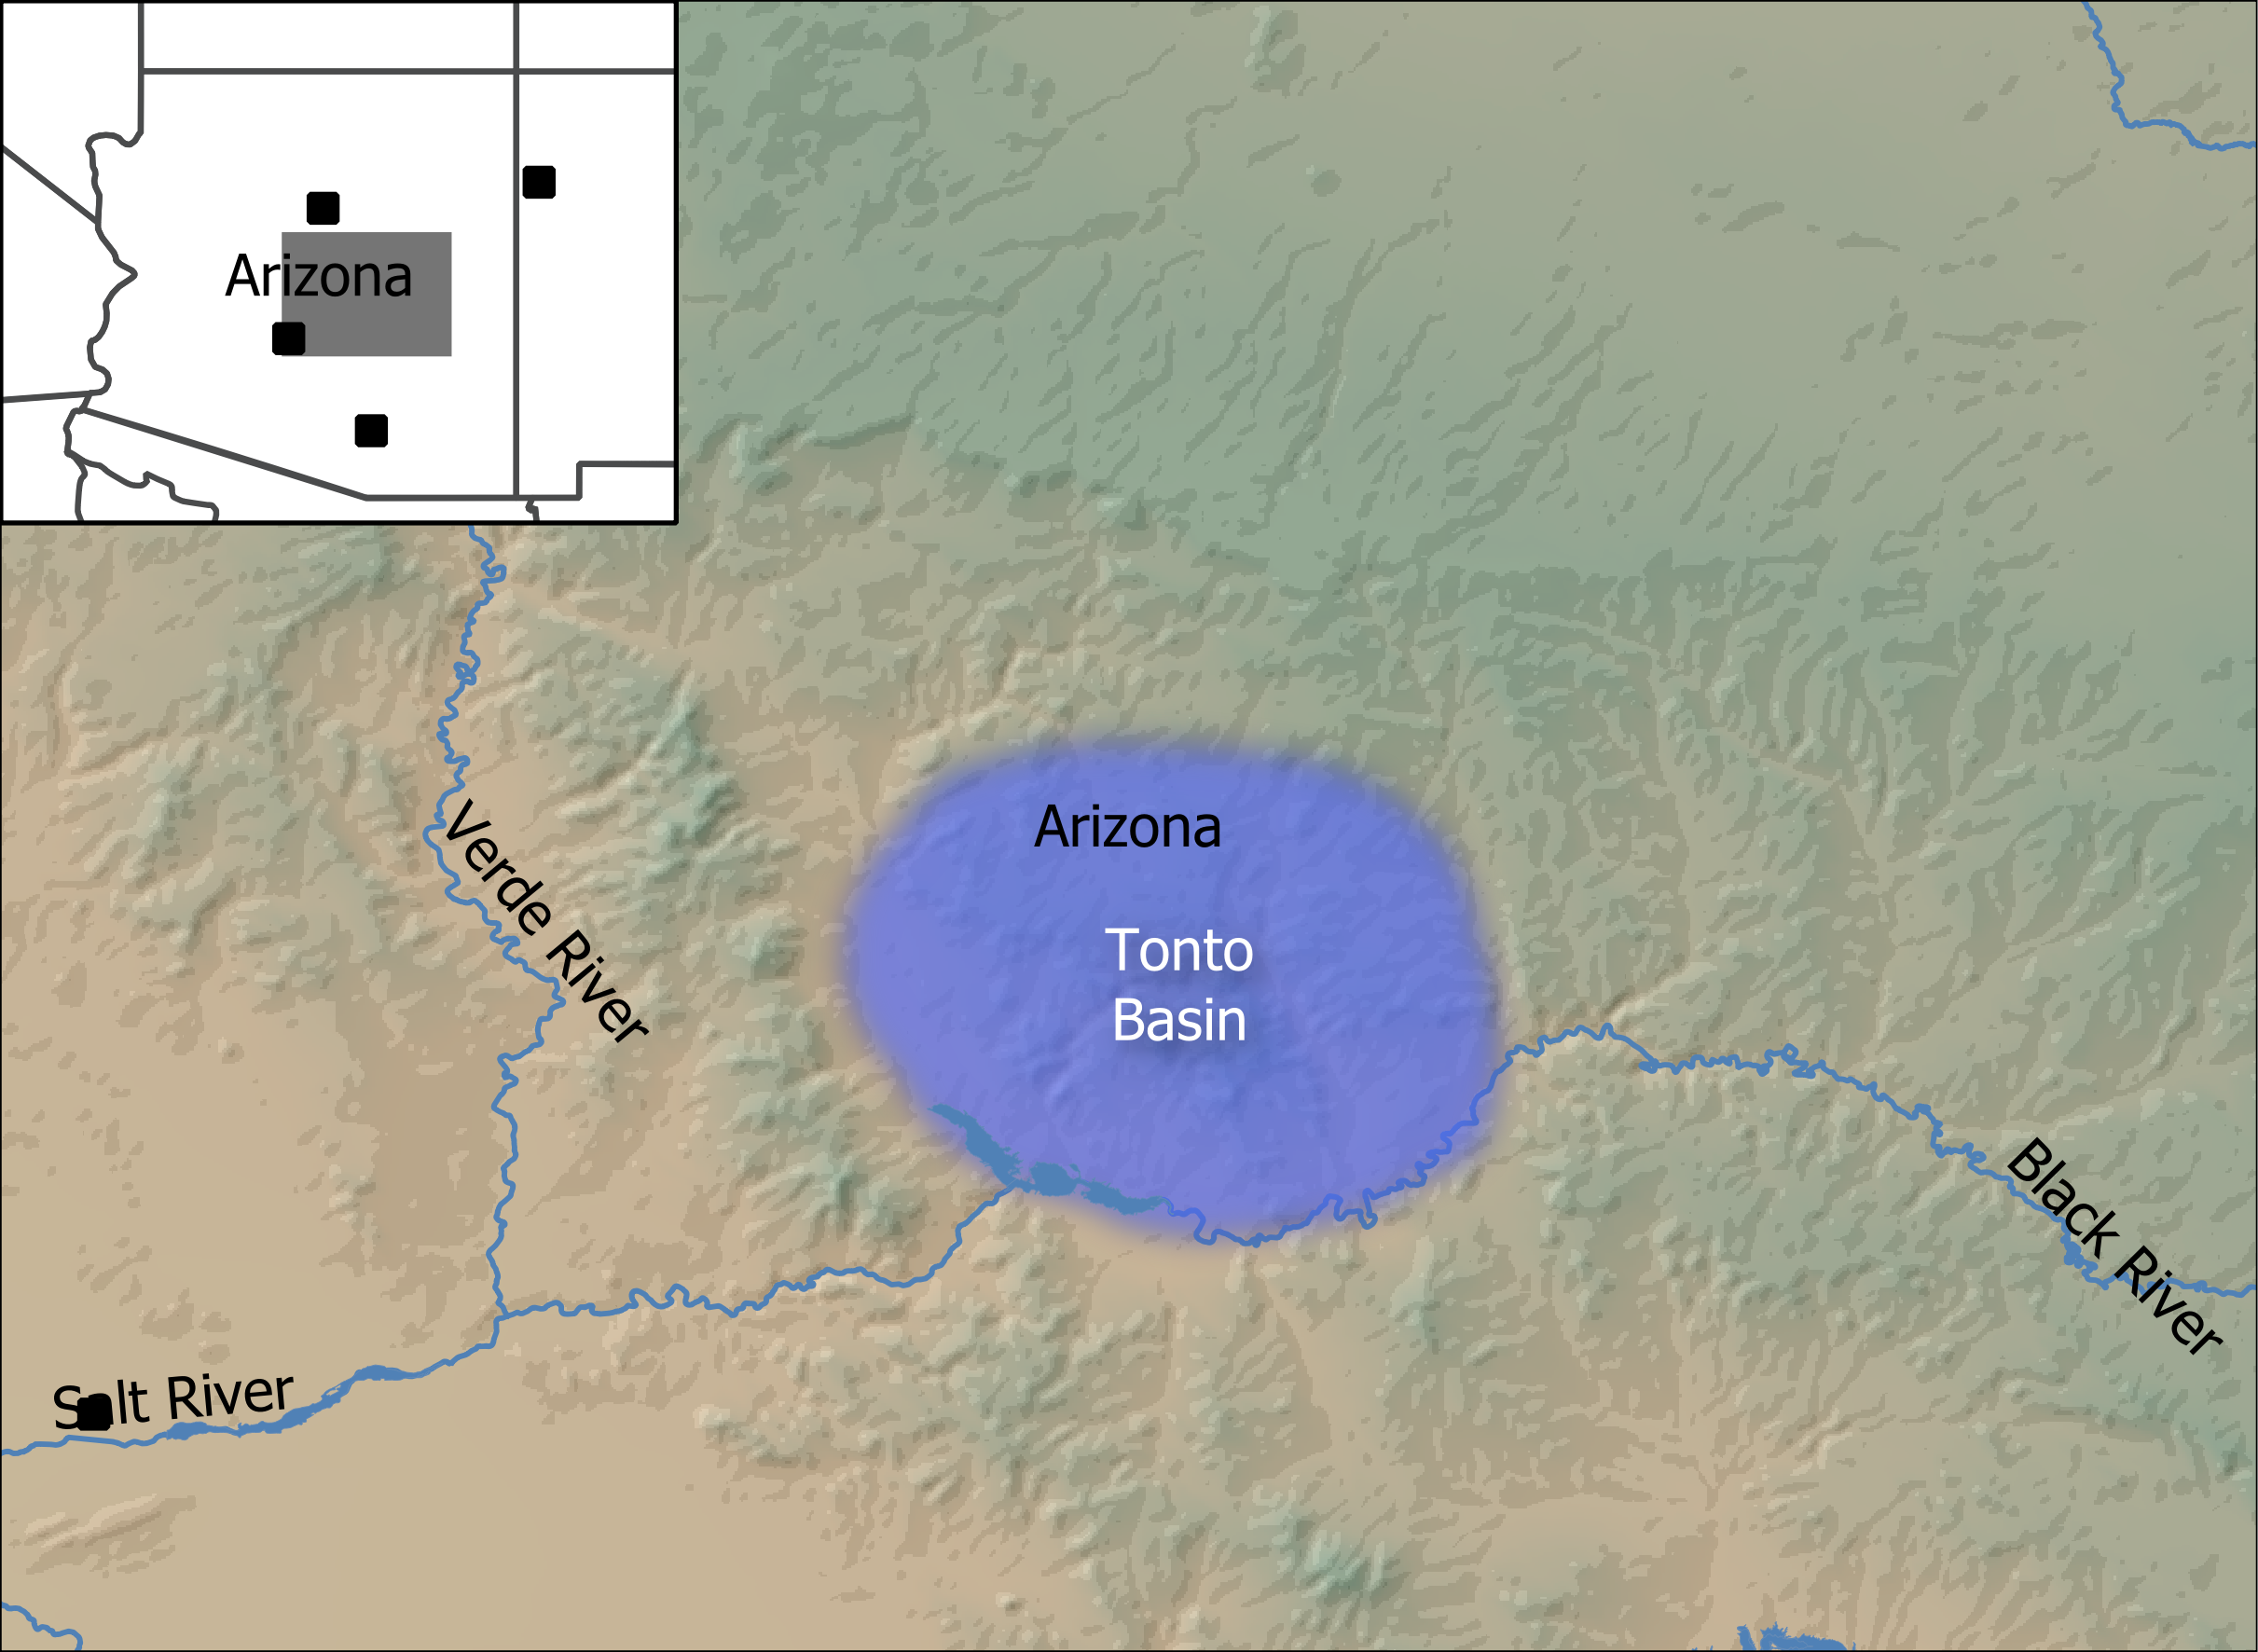
\includegraphics[width=1\linewidth]{figures/Tonto Basin} \caption{Location of Tonto Basin in the state of Arizona, United States.}\label{fig:TontoBasinMap}
\end{figure}

This is an exploratory analysis designed to minimize the amount of time
spent collecting data and to be as reproducible as possible. There are a
number of research steps that are often not addressed in publications.
This missing documentation can make reproducing results challenging.
Some of the minutiae, including the R code used in the analysis, will be
detailed in the supplemental material, but I will describe the rational
for relevant decisions.

One of the key elements of this study is reproducibility, which
necessitates automation. Projectile point analysis often includes
assigning a point to a type based on linear metrics--sometimes angular
measurements as well, and the presence or absence of various features
(e.g., concave base, serrated blades, corner-notches). But often, the
analyst is left to visually compare the point to various type specimens
to identify the closest match. In my experience, this can be a
frustrating way to spend your time. This method is harder to reproduce
and subject to greater human error. Yet, algorithms are only part of the
answer, and human judgment and context are still critical to any
analysis. The key is to minimize the possibilities for error and
maximize the opportunities for reproducibility, which I have tried to do
here. Thus, one of the key questions of this research is to determine
what input should be left to the analyst and what can be left to
automated or standardized procedures.

\hypertarget{data-collection}{%
\subsection{Data collection}\label{data-collection}}

This study has two sources of data: illustrations of projectile points
published by Justice (\protect\hyperlink{ref-Justice2002-cf}{2002}) and
images of projectile points from collection held at Arizona State
University. The datasets include 74 illustrations from Justice's
publication and 90 projectile points from Tonto Basin. Many of Justice's
types could not be included because there were so few complete,
illustrated examples.

It is worthwhile to question how an illustration compares to an image of
a physical projectile point obtained from a flatbed scanner.
Fortunately, illustrations have been published for some of the
projectile points in this study. Figure 2 is a comparison of outlines
created from an illustration and scan of the same projectile point.
There are subtle differences between the two mediums--the base is
slightly more rounded in places than the scan. These differences are
detectable in a morphometrics analysis, however, the differences are
minor as seen in figure 3. The quality of projectile point illustration
can vary, but from this brief comparison there should be no hesitation
using illustrations for 2D morphometric analysis.

\begin{figure}
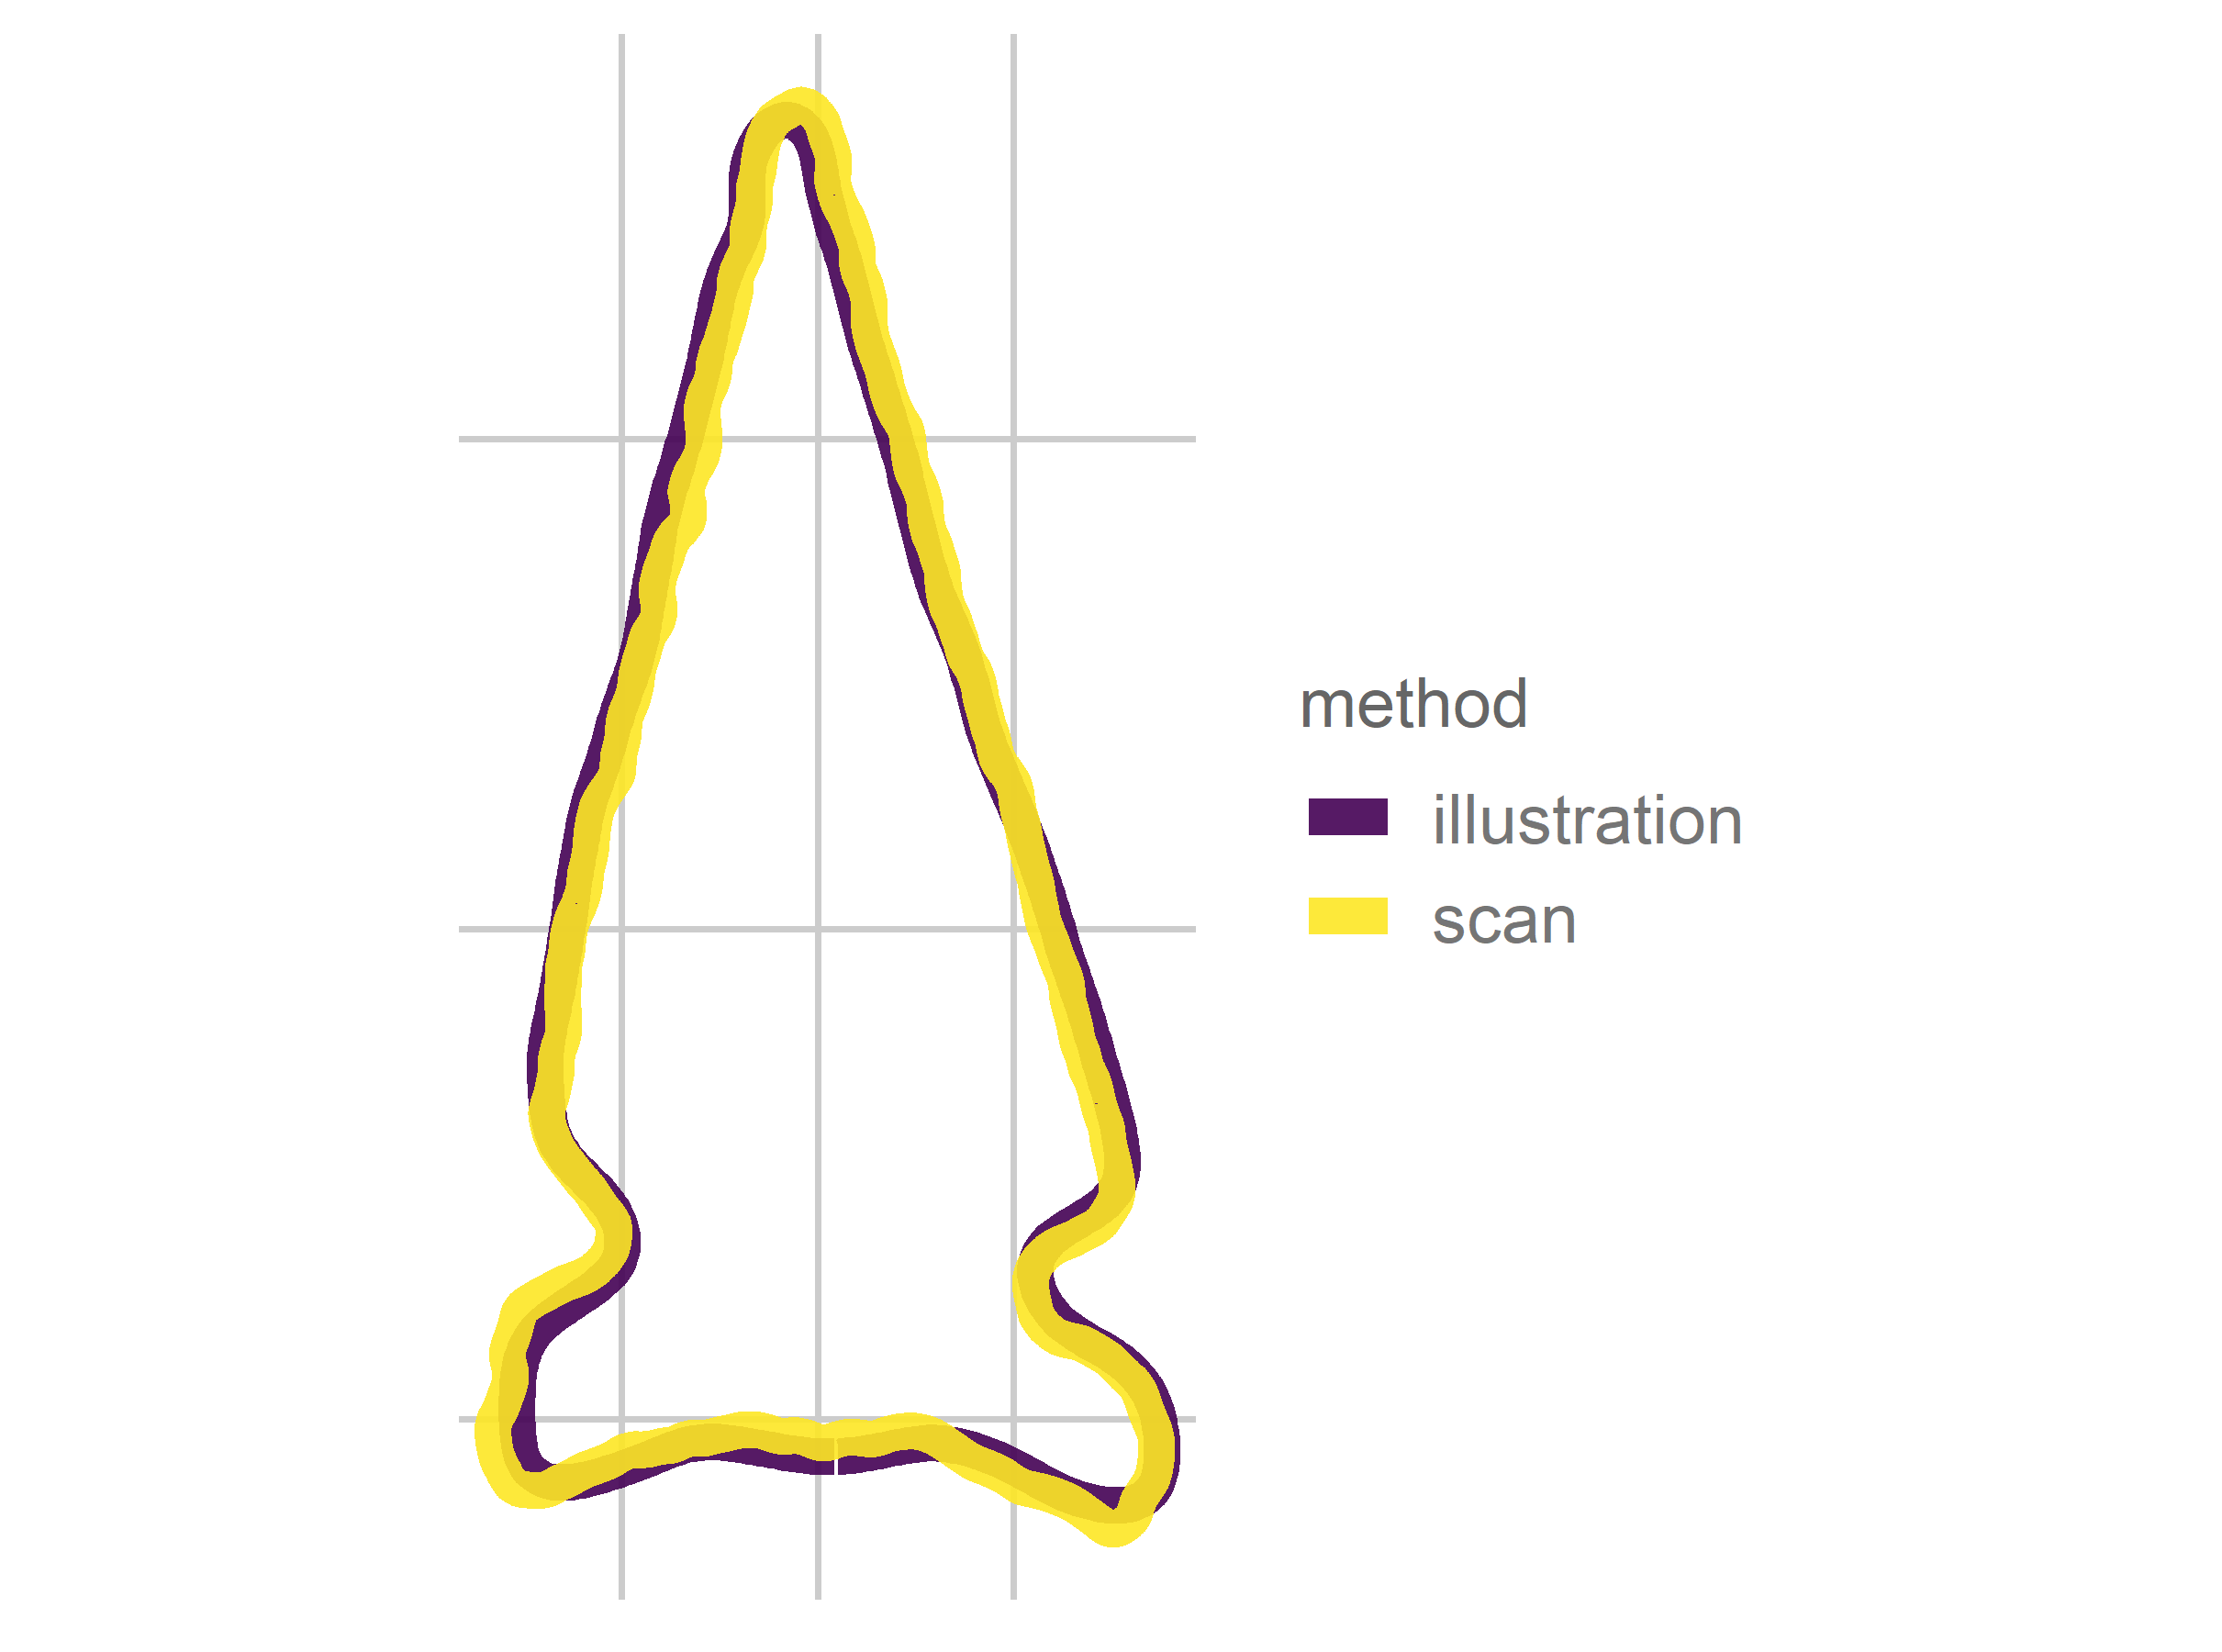
\includegraphics[width=1\linewidth]{figures/pointComparison} \caption{Comparison of projectile point outlines for an illustration and a scan of the same projectile point (Oliver and Simon 1997: Figure 9.3; Specimen 33598)}\label{fig:pointComparison}
\end{figure}

\begin{figure}
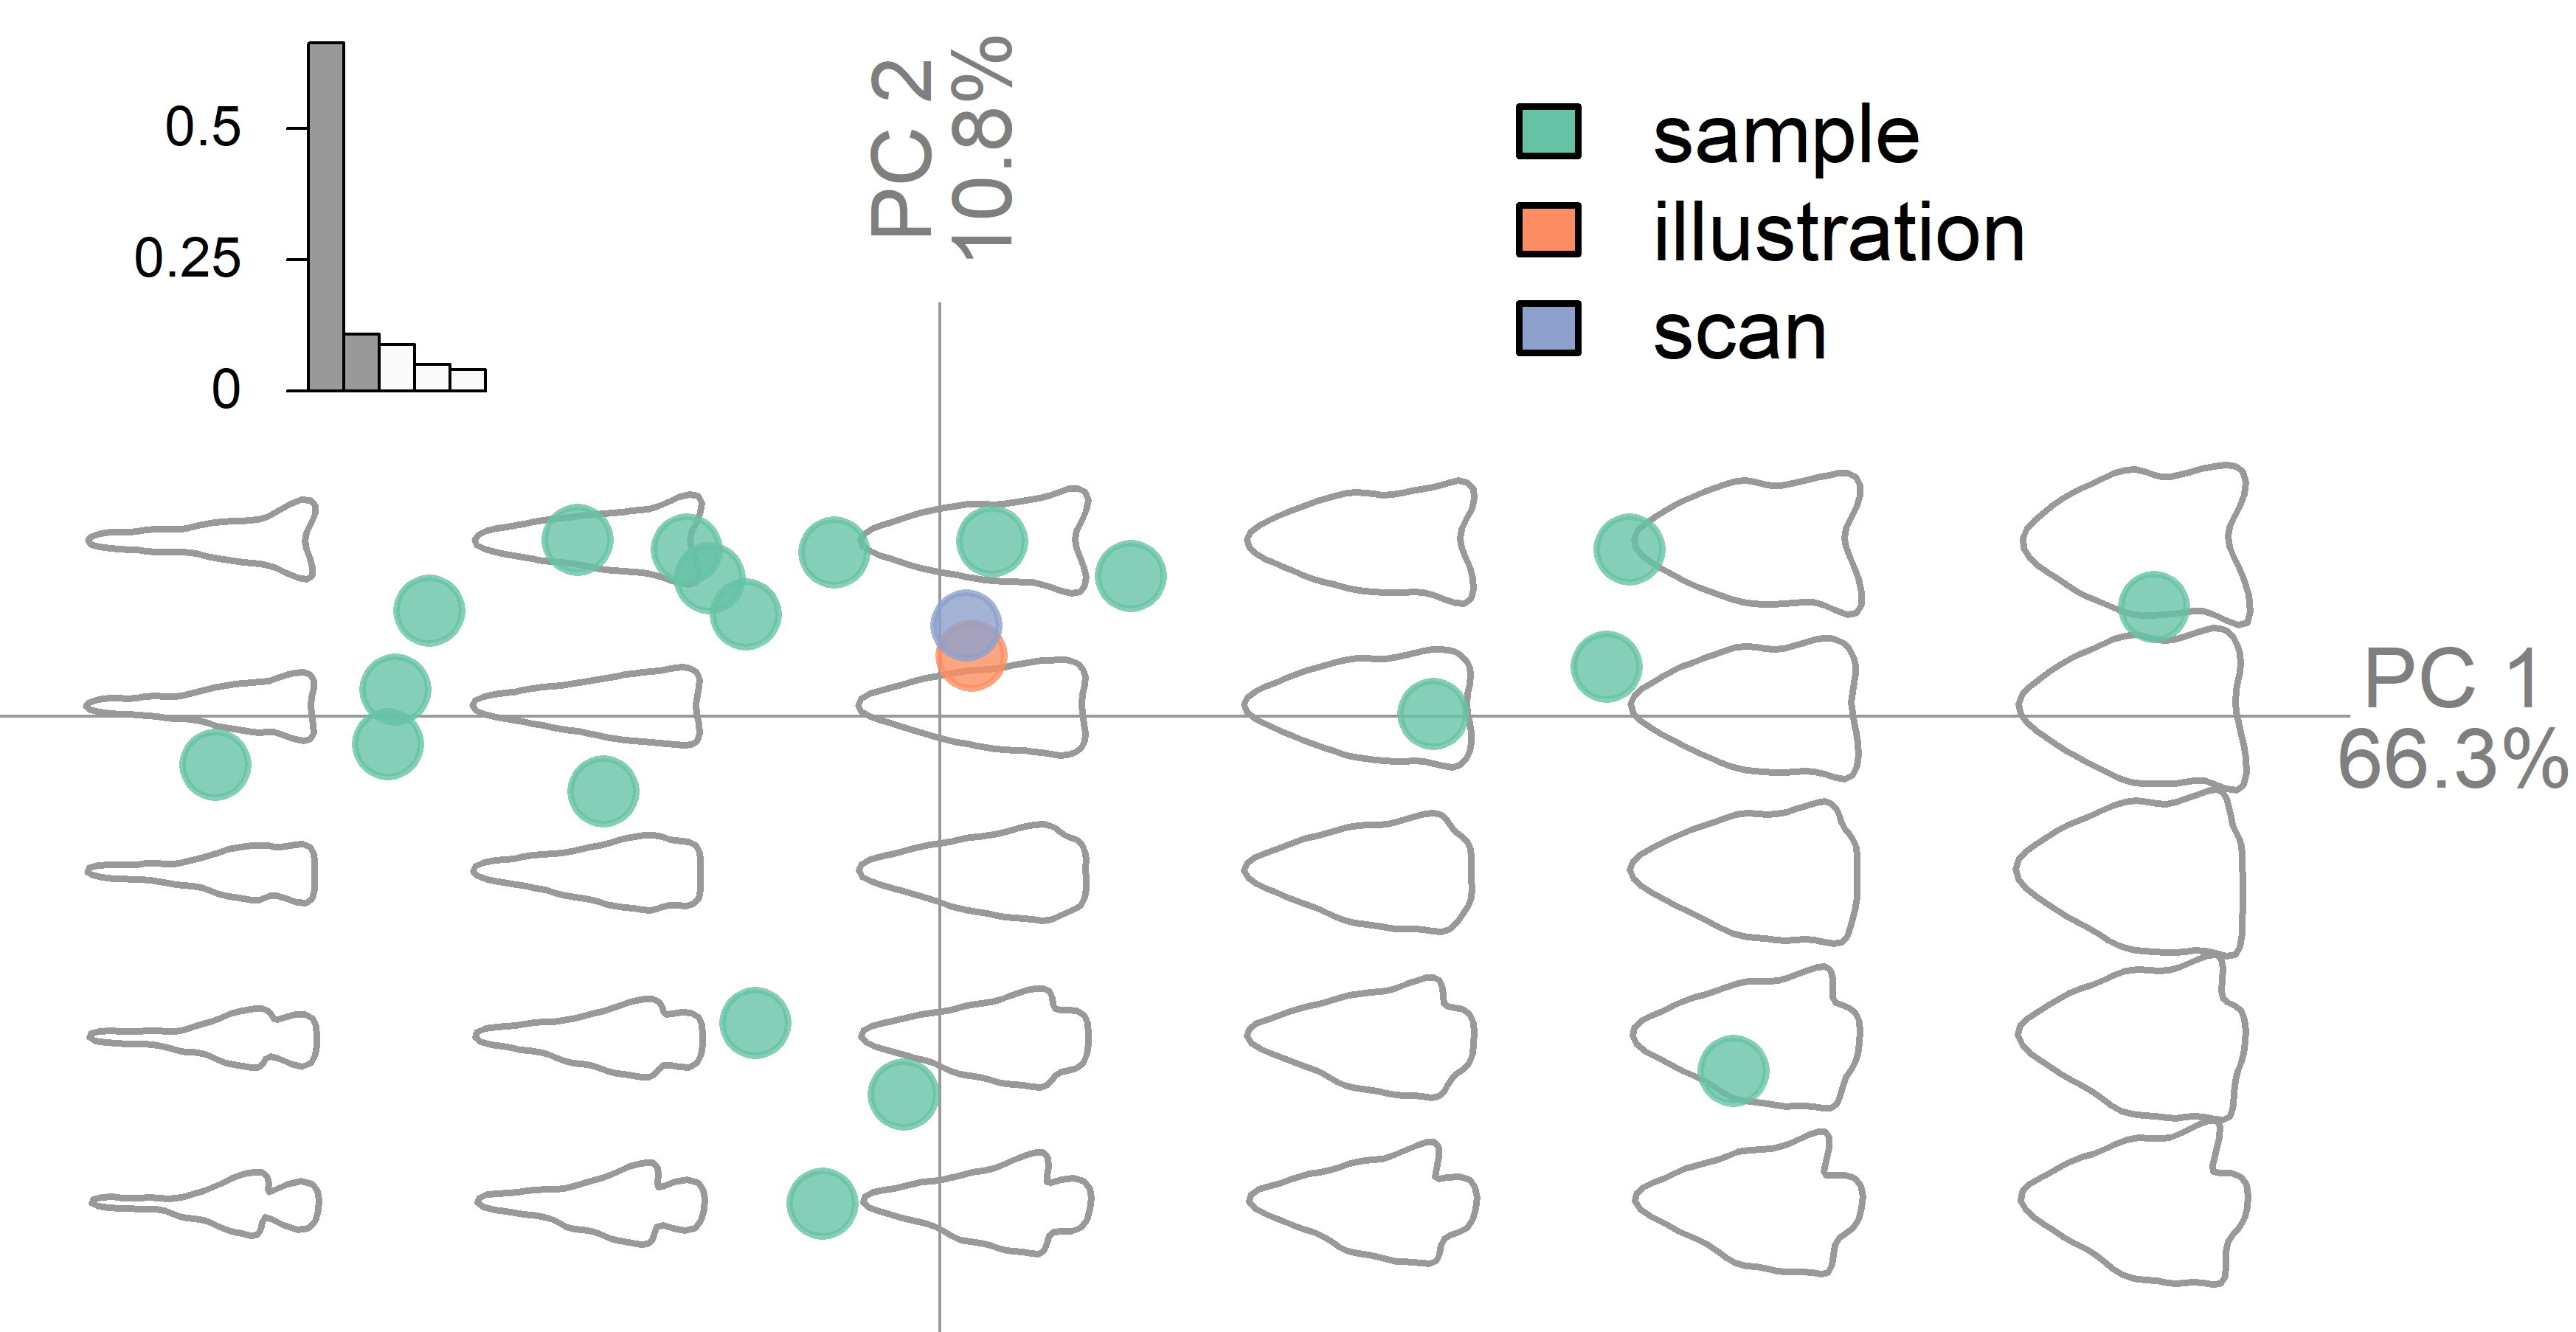
\includegraphics[width=1\linewidth]{figures/comparisonPCA} \caption{Principal component plot comparing the morphometric differences between a sample of 20 random projectile points and the illustration and scan of the same projectile point.}\label{fig:comparisonPCA}
\end{figure}

Justice's projectile point illustrations were scanned, and the
illustrations were converted into individual, solid black outlines and
saved as jpeg files using common image-editing software. The open source
statistical software R was used for all analyses
(\protect\hyperlink{ref-R_Core_Team2022-wb}{R Core Team 2022}). The
Momocs package (\protect\hyperlink{ref-Bonhomme2014-gt}{Bonhomme et al.
2014}) has an import function to convert jpeg files into outlines. This
is a major advantage over manual outlining processes used in popular GM
software, such as tpsDig
(\protect\hyperlink{ref-James_Rohlf2015-ui}{James Rohlf 2015}). These
outlines form the the basis of the geometric morphometric analyses
conducted here with the exception of the landmark analyses. Landmarking
was performed using the tpsDig software. The Momocs package has that
capability, but I have found tpsDig's utility for landmarking to be
superior. The Tonto Basin projectile point images were created using a
flatbed scanner at 1200 DPI \footnote{Many of the images were obtained
  by the author but some were generously contributed by Josh Watts--see
  the results of his study here:
  (\protect\hyperlink{ref-Watts2013-ub}{Watts 2013}).}. The images were
converted to outlines using the same process as the projectile point
illustrations.

\hypertarget{projectile-points-of-the-southwest}{%
\subsection{Projectile points of the
Southwest}\label{projectile-points-of-the-southwest}}

There are a few regional typologies for projectile points in the
Southwest: common examples were authored by Hoffman
(\protect\hyperlink{ref-Hoffman1997-hb}{1997}), Justice
(\protect\hyperlink{ref-Justice2002-cf}{2002}), Loendorf and Rice
(\protect\hyperlink{ref-Loendorf2004-tp}{2004}), and Sliva
(\protect\hyperlink{ref-Sliva2006-nq}{2006}). Altogether, these four
typologies include 129 projectile point types, although many overlap. In
some cases, the authors identify correlates of the types. Many types
date to the Archaic period, and thus predate the primary period we are
interested in. Not all of the points were ascribed dates by the authors.
Justice lists 23 points that overlap with the AD 1100-1500 period (the
maximal dates for the Hohokam Classic period). Projectile points have
restricted geographical boundaries, although these boundaries correspond
to much greater areas than ceramic types typically do
(\protect\hyperlink{ref-Buchanan2019-vn}{Buchanan et al. 2019}). Figure
4 shows that several projectile point boundaries defined by Justice
overlap with the Tonto Basin.

\begin{figure}
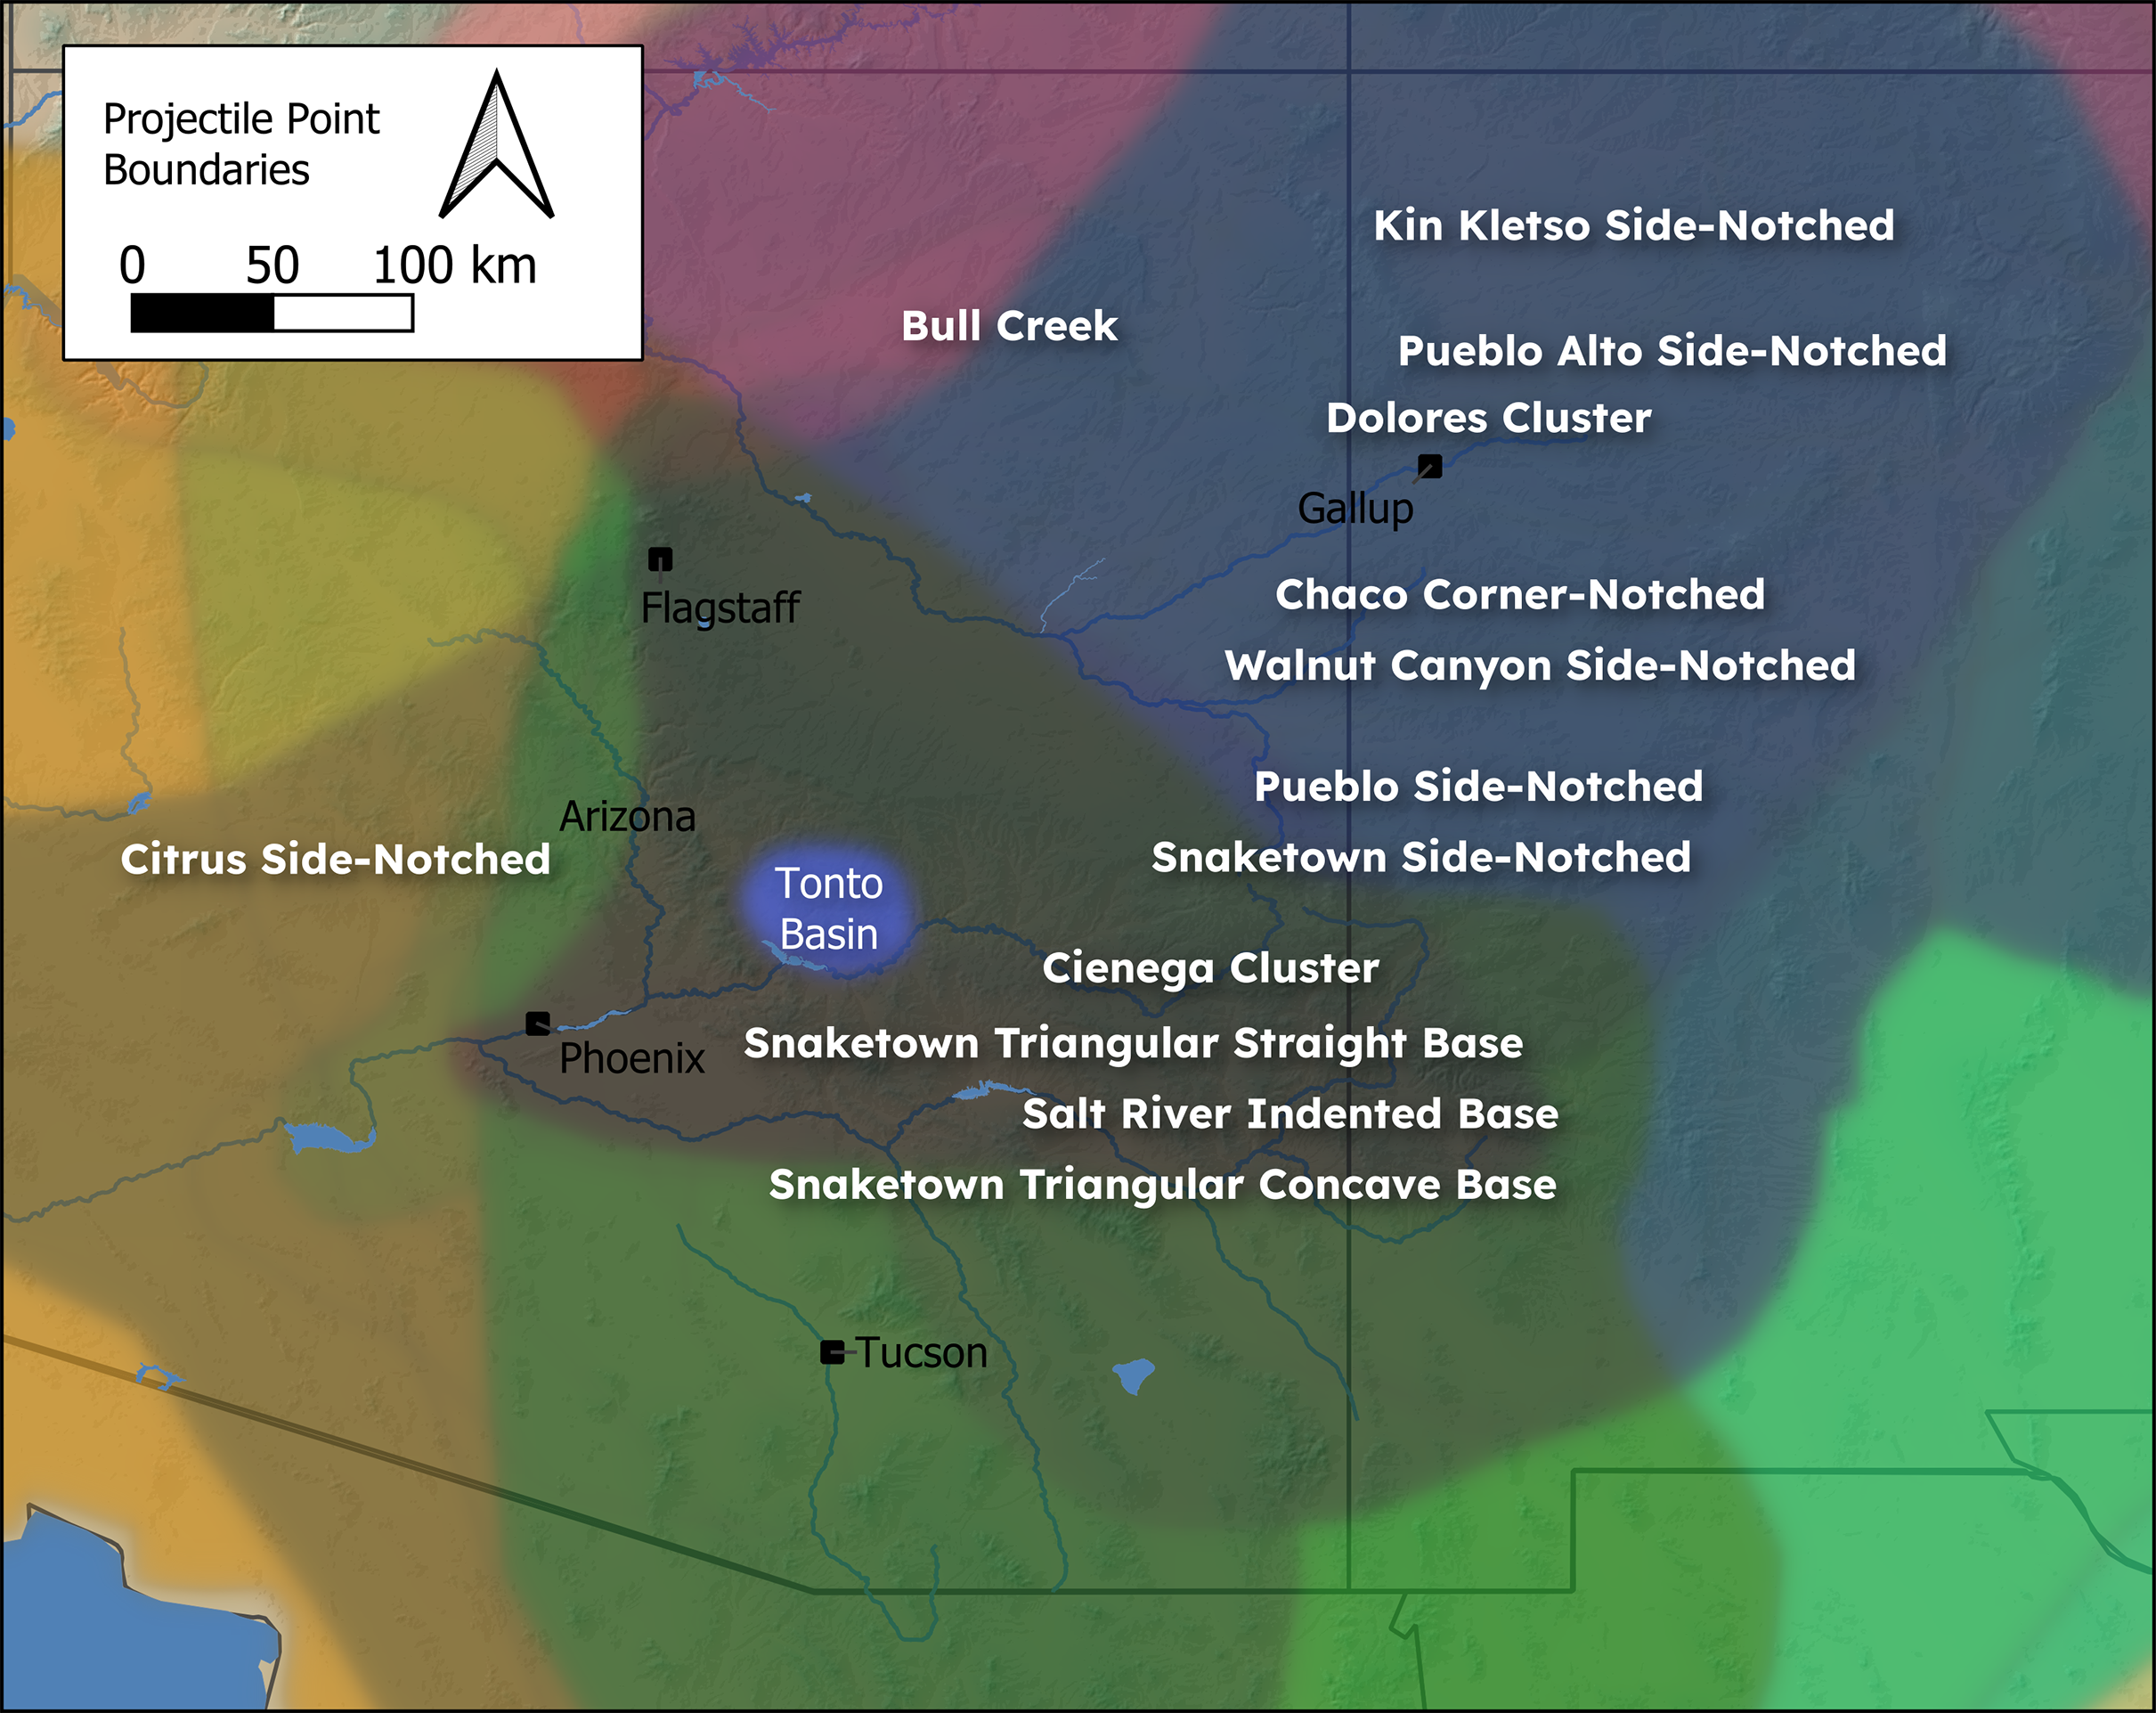
\includegraphics[width=1\linewidth]{figures/ProjPointBoundaries} \caption{Location of selected projectile point boundaries defined by Justice (2002) as digitized by Buchanan and colleagues (2019). Darker colors represent greater overlap in the number of projectile point boundaries.}\label{fig:ProjectilePointBoundaries}
\end{figure}

For this study, I digitized 74 projectile point images from Justice's
publication representing 8 projectile point types (table 1). Justice
placed each projectile point type into a cluster of related points.
Figure 5 shows the projectile point outlines by type. The included
projectile point types include some Archaic points and types not
expected to overlap with the Tonto Basin projectile points. Archaic
points are often found at later sites, and these types form useful
comparisons, as they should not match to non-archaic projectile points.
One limitation of this study is that projectile points must be complete,
or nearly complete (minor damage to the tip or another part of the point
that was judged to not significantly impact the shape of the point was
ignored). Thus, not all of the illustrations included in Justice's book
could be included in the outline analyses.

 
  \providecommand{\huxb}[2]{\arrayrulecolor[RGB]{#1}\global\arrayrulewidth=#2pt}
  \providecommand{\huxvb}[2]{\color[RGB]{#1}\vrule width #2pt}
  \providecommand{\huxtpad}[1]{\rule{0pt}{#1}}
  \providecommand{\huxbpad}[1]{\rule[-#1]{0pt}{#1}}

\begin{table}[ht]
\begin{centerbox}
\begin{threeparttable}
\captionsetup{justification=centering,singlelinecheck=off}
\caption{Cluster Names, Types, and Number of Samples}
 \label{tab:tblJusticeTypes}
\setlength{\tabcolsep}{0pt}
\begin{tabular}{l l l}


\hhline{}
\arrayrulecolor{black}

\multicolumn{1}{!{\huxvb{0, 0, 0}{0}}l!{\huxvb{0, 0, 0}{0}}}{\huxtpad{1pt + 1em}\raggedright \hspace{0pt} \textbf{Cluster} \hspace{1pt}\huxbpad{1pt}} &
\multicolumn{1}{l!{\huxvb{0, 0, 0}{0}}}{\huxtpad{1pt + 1em}\raggedright \hspace{1pt} \textbf{Type} \hspace{1pt}\huxbpad{1pt}} &
\multicolumn{1}{r!{\huxvb{0, 0, 0}{0}}}{\huxtpad{1pt + 1em}\raggedleft \hspace{1pt} \textbf{total} \hspace{0pt}\huxbpad{1pt}} \tabularnewline[-0.5pt]


\hhline{>{\huxb{0, 0, 0}{0.4}}->{\huxb{0, 0, 0}{0.4}}->{\huxb{0, 0, 0}{0.4}}-}
\arrayrulecolor{black}

\multicolumn{1}{!{\huxvb{0, 0, 0}{0}}l!{\huxvb{0, 0, 0}{0}}}{\huxtpad{1pt + 1em}\raggedright \hspace{0pt} Chaco \hspace{1pt}\huxbpad{1pt}} &
\multicolumn{1}{l!{\huxvb{0, 0, 0}{0}}}{\huxtpad{1pt + 1em}\raggedright \hspace{1pt} Chaco Corner Notched \hspace{1pt}\huxbpad{1pt}} &
\multicolumn{1}{r!{\huxvb{0, 0, 0}{0}}}{\huxtpad{1pt + 1em}\raggedleft \hspace{1pt} 9 \hspace{0pt}\huxbpad{1pt}} \tabularnewline[-0.5pt]


\hhline{}
\arrayrulecolor{black}

\multicolumn{1}{!{\huxvb{0, 0, 0}{0}}l!{\huxvb{0, 0, 0}{0}}}{\huxtpad{1pt + 1em}\raggedright \hspace{0pt} Chaco \hspace{1pt}\huxbpad{1pt}} &
\multicolumn{1}{l!{\huxvb{0, 0, 0}{0}}}{\huxtpad{1pt + 1em}\raggedright \hspace{1pt} Pueblo Alto Side Notched \hspace{1pt}\huxbpad{1pt}} &
\multicolumn{1}{r!{\huxvb{0, 0, 0}{0}}}{\huxtpad{1pt + 1em}\raggedleft \hspace{1pt} 7 \hspace{0pt}\huxbpad{1pt}} \tabularnewline[-0.5pt]


\hhline{}
\arrayrulecolor{black}

\multicolumn{1}{!{\huxvb{0, 0, 0}{0}}l!{\huxvb{0, 0, 0}{0}}}{\huxtpad{1pt + 1em}\raggedright \hspace{0pt} Cienega \hspace{1pt}\huxbpad{1pt}} &
\multicolumn{1}{l!{\huxvb{0, 0, 0}{0}}}{\huxtpad{1pt + 1em}\raggedright \hspace{1pt} Tularosa Corner Notched \hspace{1pt}\huxbpad{1pt}} &
\multicolumn{1}{r!{\huxvb{0, 0, 0}{0}}}{\huxtpad{1pt + 1em}\raggedleft \hspace{1pt} 13 \hspace{0pt}\huxbpad{1pt}} \tabularnewline[-0.5pt]


\hhline{}
\arrayrulecolor{black}

\multicolumn{1}{!{\huxvb{0, 0, 0}{0}}l!{\huxvb{0, 0, 0}{0}}}{\huxtpad{1pt + 1em}\raggedright \hspace{0pt} Livermore \hspace{1pt}\huxbpad{1pt}} &
\multicolumn{1}{l!{\huxvb{0, 0, 0}{0}}}{\huxtpad{1pt + 1em}\raggedright \hspace{1pt} Guadalupe \hspace{1pt}\huxbpad{1pt}} &
\multicolumn{1}{r!{\huxvb{0, 0, 0}{0}}}{\huxtpad{1pt + 1em}\raggedleft \hspace{1pt} 12 \hspace{0pt}\huxbpad{1pt}} \tabularnewline[-0.5pt]


\hhline{}
\arrayrulecolor{black}

\multicolumn{1}{!{\huxvb{0, 0, 0}{0}}l!{\huxvb{0, 0, 0}{0}}}{\huxtpad{1pt + 1em}\raggedright \hspace{0pt} Pueblo Side Notched \hspace{1pt}\huxbpad{1pt}} &
\multicolumn{1}{l!{\huxvb{0, 0, 0}{0}}}{\huxtpad{1pt + 1em}\raggedright \hspace{1pt} Pueblo Side Notched Concave Base \hspace{1pt}\huxbpad{1pt}} &
\multicolumn{1}{r!{\huxvb{0, 0, 0}{0}}}{\huxtpad{1pt + 1em}\raggedleft \hspace{1pt} 9 \hspace{0pt}\huxbpad{1pt}} \tabularnewline[-0.5pt]


\hhline{}
\arrayrulecolor{black}

\multicolumn{1}{!{\huxvb{0, 0, 0}{0}}l!{\huxvb{0, 0, 0}{0}}}{\huxtpad{1pt + 1em}\raggedright \hspace{0pt} Pueblo Side Notched \hspace{1pt}\huxbpad{1pt}} &
\multicolumn{1}{l!{\huxvb{0, 0, 0}{0}}}{\huxtpad{1pt + 1em}\raggedright \hspace{1pt} Pueblo Side Notched Straight Base \hspace{1pt}\huxbpad{1pt}} &
\multicolumn{1}{r!{\huxvb{0, 0, 0}{0}}}{\huxtpad{1pt + 1em}\raggedleft \hspace{1pt} 7 \hspace{0pt}\huxbpad{1pt}} \tabularnewline[-0.5pt]


\hhline{}
\arrayrulecolor{black}

\multicolumn{1}{!{\huxvb{0, 0, 0}{0}}l!{\huxvb{0, 0, 0}{0}}}{\huxtpad{1pt + 1em}\raggedright \hspace{0pt} Snaketown \hspace{1pt}\huxbpad{1pt}} &
\multicolumn{1}{l!{\huxvb{0, 0, 0}{0}}}{\huxtpad{1pt + 1em}\raggedright \hspace{1pt} Snaketown Triangular Concave Base \hspace{1pt}\huxbpad{1pt}} &
\multicolumn{1}{r!{\huxvb{0, 0, 0}{0}}}{\huxtpad{1pt + 1em}\raggedleft \hspace{1pt} 9 \hspace{0pt}\huxbpad{1pt}} \tabularnewline[-0.5pt]


\hhline{}
\arrayrulecolor{black}

\multicolumn{1}{!{\huxvb{0, 0, 0}{0}}l!{\huxvb{0, 0, 0}{0}}}{\huxtpad{1pt + 1em}\raggedright \hspace{0pt} Western Triangular \hspace{1pt}\huxbpad{1pt}} &
\multicolumn{1}{l!{\huxvb{0, 0, 0}{0}}}{\huxtpad{1pt + 1em}\raggedright \hspace{1pt} Cottonwood Triangular \hspace{1pt}\huxbpad{1pt}} &
\multicolumn{1}{r!{\huxvb{0, 0, 0}{0}}}{\huxtpad{1pt + 1em}\raggedleft \hspace{1pt} 8 \hspace{0pt}\huxbpad{1pt}} \tabularnewline[-0.5pt]


\hhline{}
\arrayrulecolor{black}
\end{tabular}
\end{threeparttable}\par\end{centerbox}

\end{table}
 

\begin{figure}
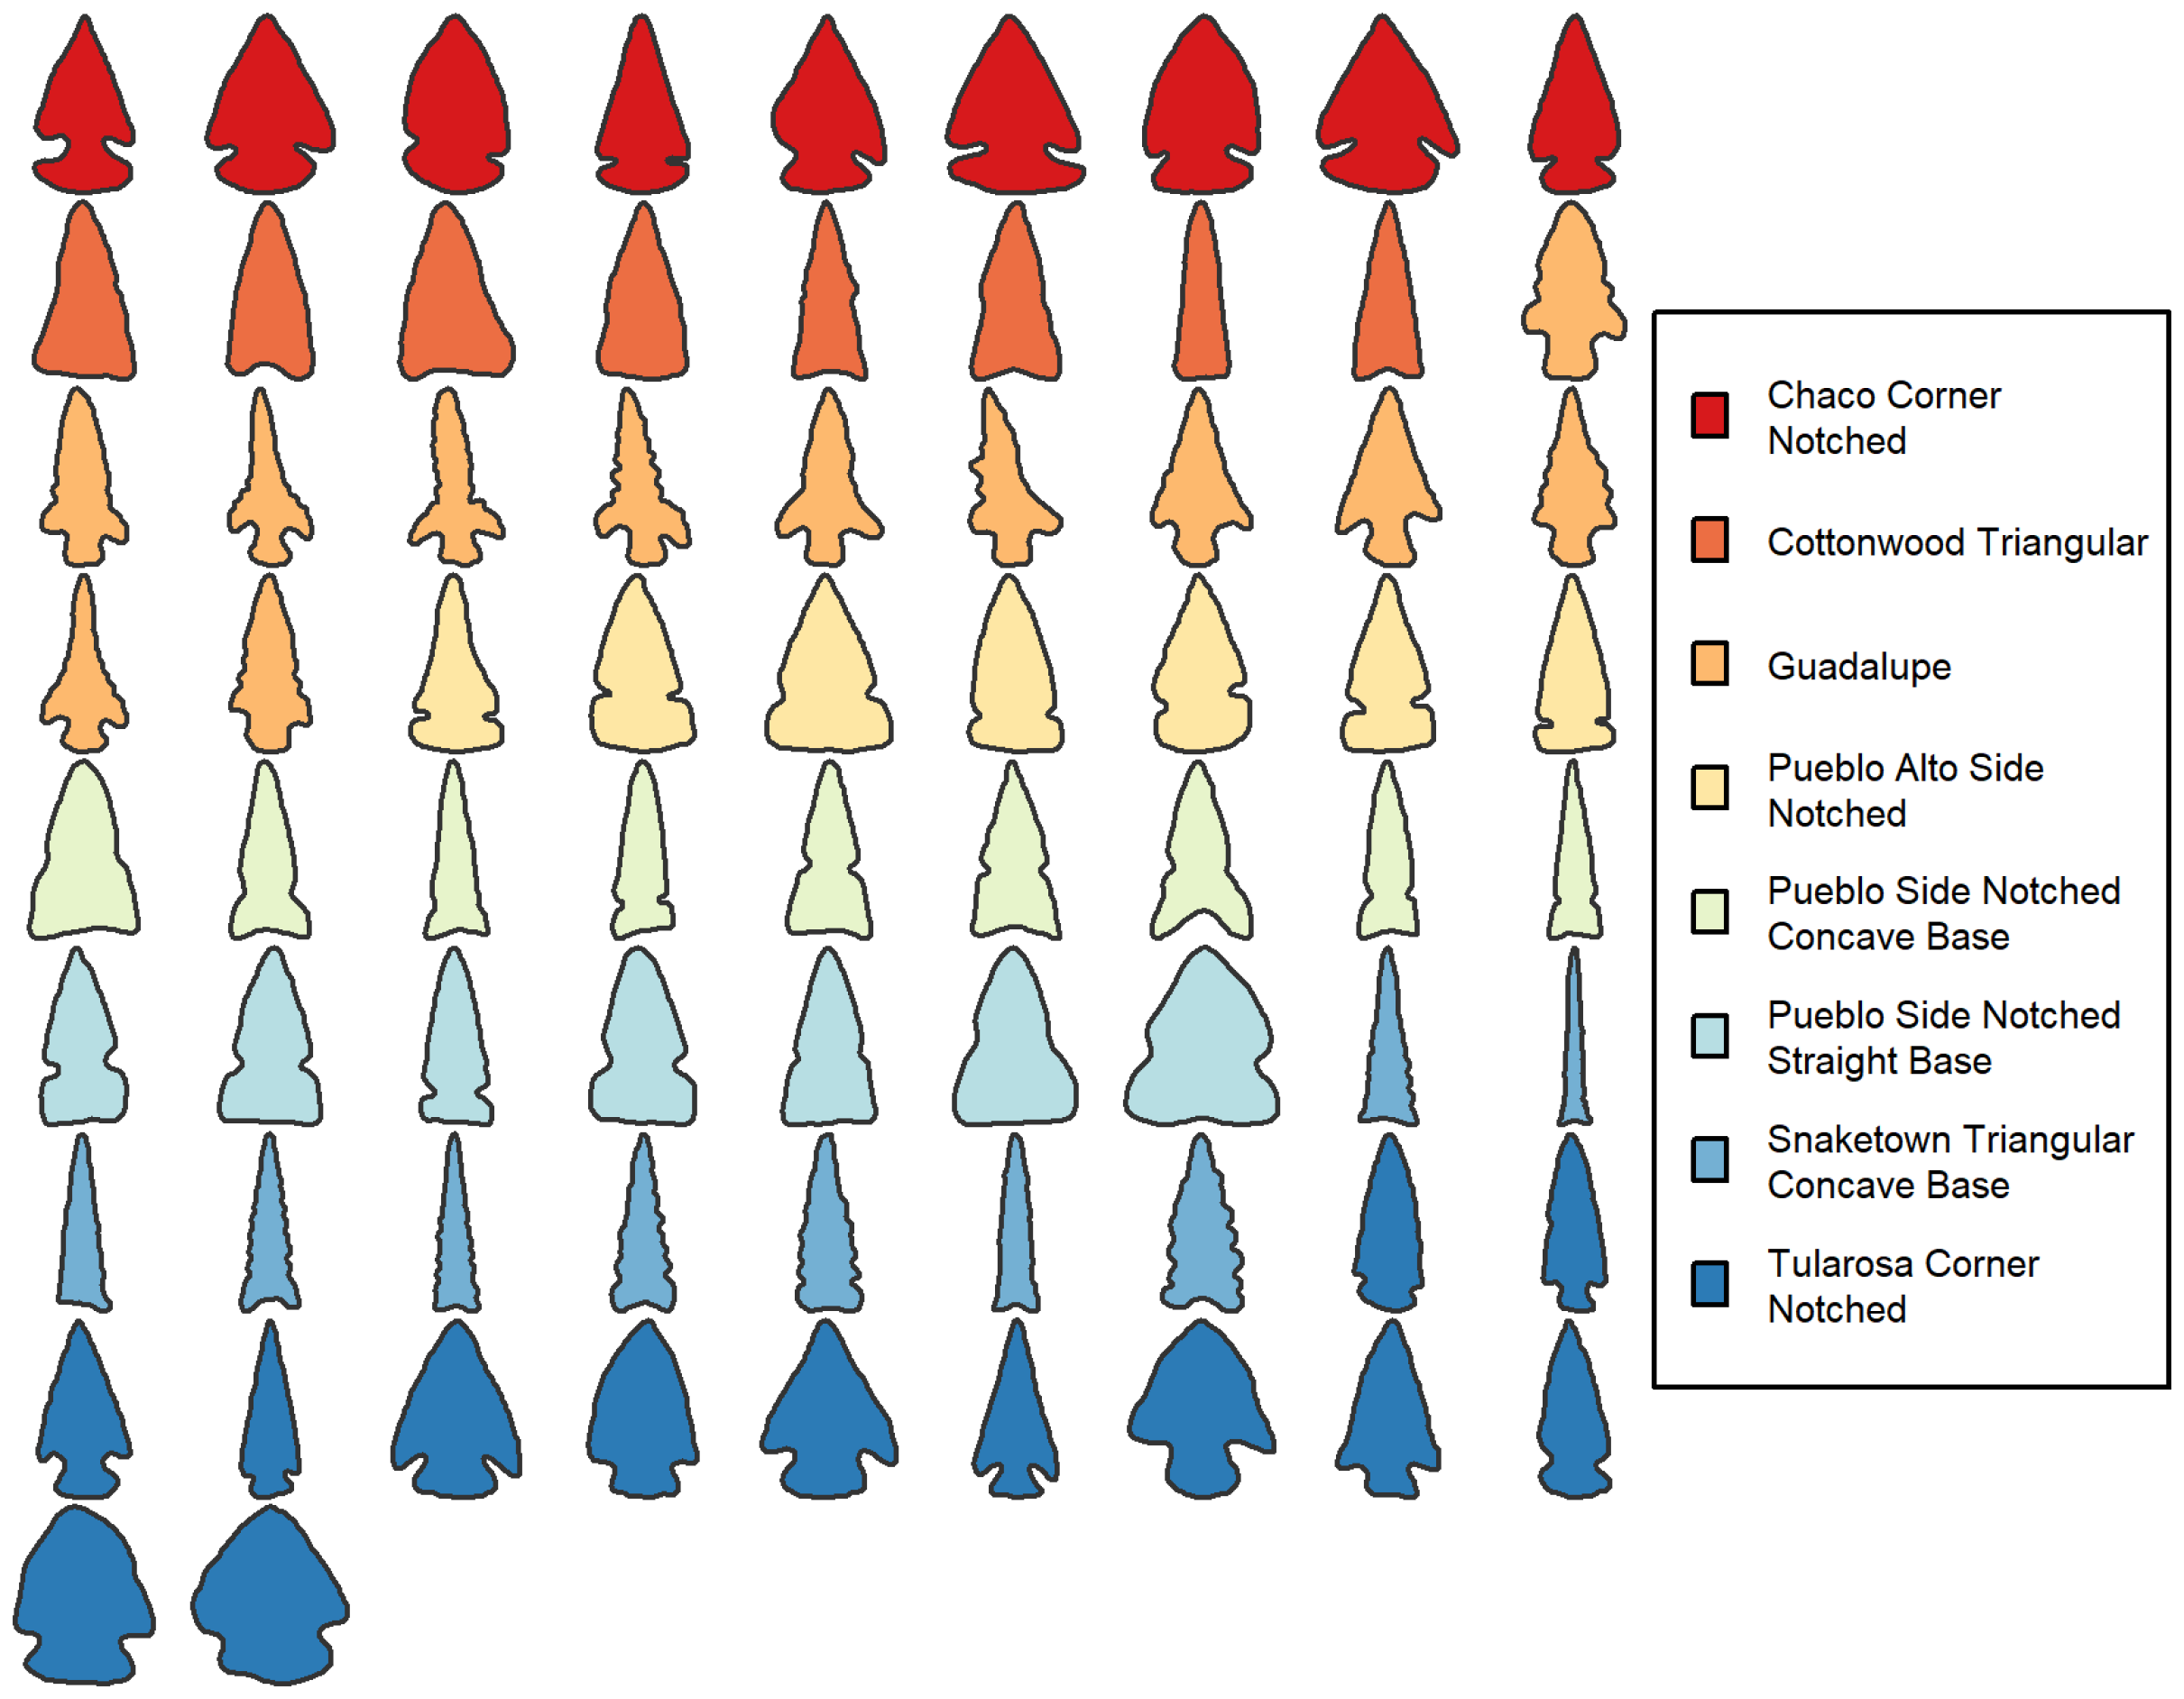
\includegraphics[width=1\linewidth]{figures/JusticePointsTypesFinal} \caption{Outlines of projectile point illustrations taken from Justice (2002). Note that the projectile points are not scaled.}\label{fig:JusticePointsTypesFinal}
\end{figure}

\hypertarget{tonto-basin-projectile-points}{%
\subsection{Tonto Basin Projectile
Points}\label{tonto-basin-projectile-points}}

The sample of Tonto Basin points used in this study come from the
Roosevelt Platform Mound Study. They come from 18 different sites that
were grouped into five clusters in the original reports (see
\protect\hyperlink{ref-Rice1998-ku}{Glen E. Rice 1998} for an overview).
Figure 6 shows the projectile points used in this study grouped by site
cluster. The majority of these sites were occupied during the Roosevelt
phase (AD 1275-1325) and early portion of the Gila phase (AD 1325-1450).
The sites consist primarily of compounds, room blocks, and platform
mounds.

\begin{figure}
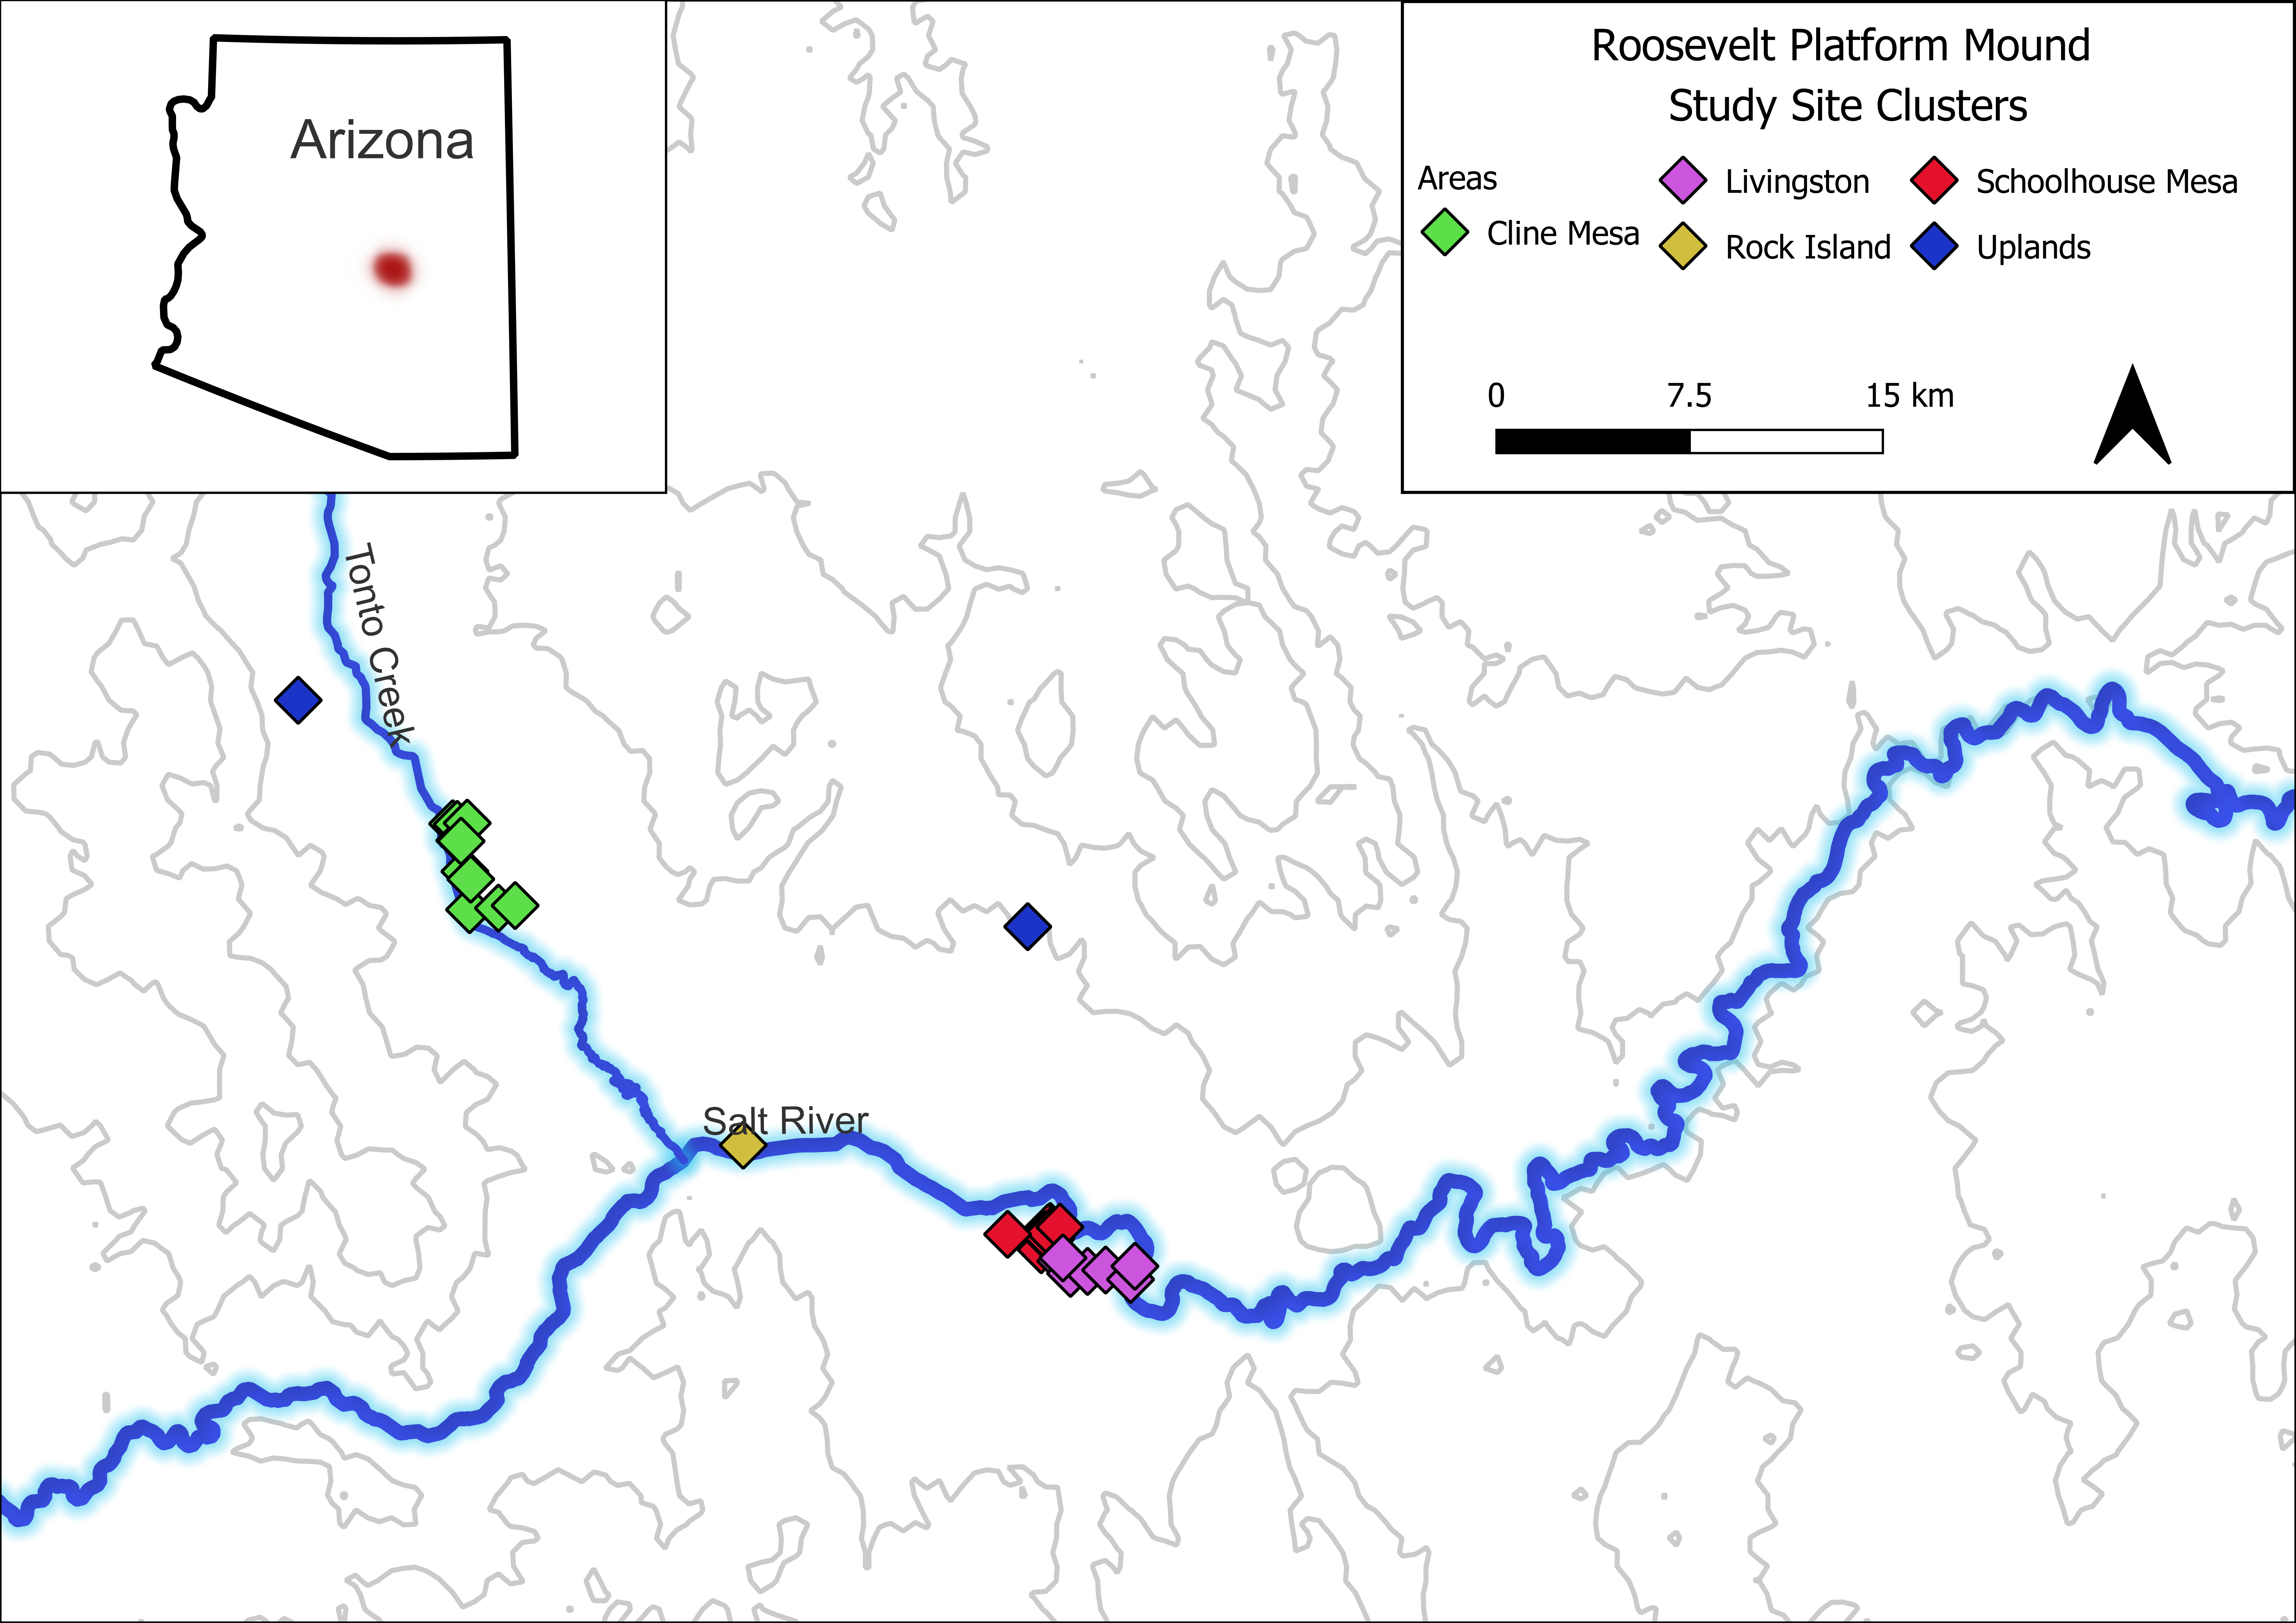
\includegraphics[width=1\linewidth]{figures/TontoBasinSitesv2} \caption{Archaeology sites from Tonto Basin included in discussion. The original reports grouped each site into different clusters. Note that two of the platform mound sites are labeled separately.}\label{fig:TontoBasinSites}
\end{figure}

The projectile points exhibit a variety of forms (see figure 7). Rice
(\protect\hyperlink{ref-Rice1994-rk}{1994}) classified Tonto Basin
points into small and large complexes (likely equivalent to dart and
arrow points), and further classified small points into the longer
Salado series and the shorter Tonto series. These series were further
subdivided using a custom classification scheme based on blade, tang,
and base shape, as well as notch style. This is a logical way to
classify the points, but it does not easily lend itself to regional
comparisons, as other points were not classified in the same way. Nearly
all of the points in the original sample consisted of side-notched or
triangular points. Because the results of the analysis discussed below
indicated that analyzing the points by shape was the most logical
choice, only the triangular and side-notched points were used in this
study.

\begin{figure}
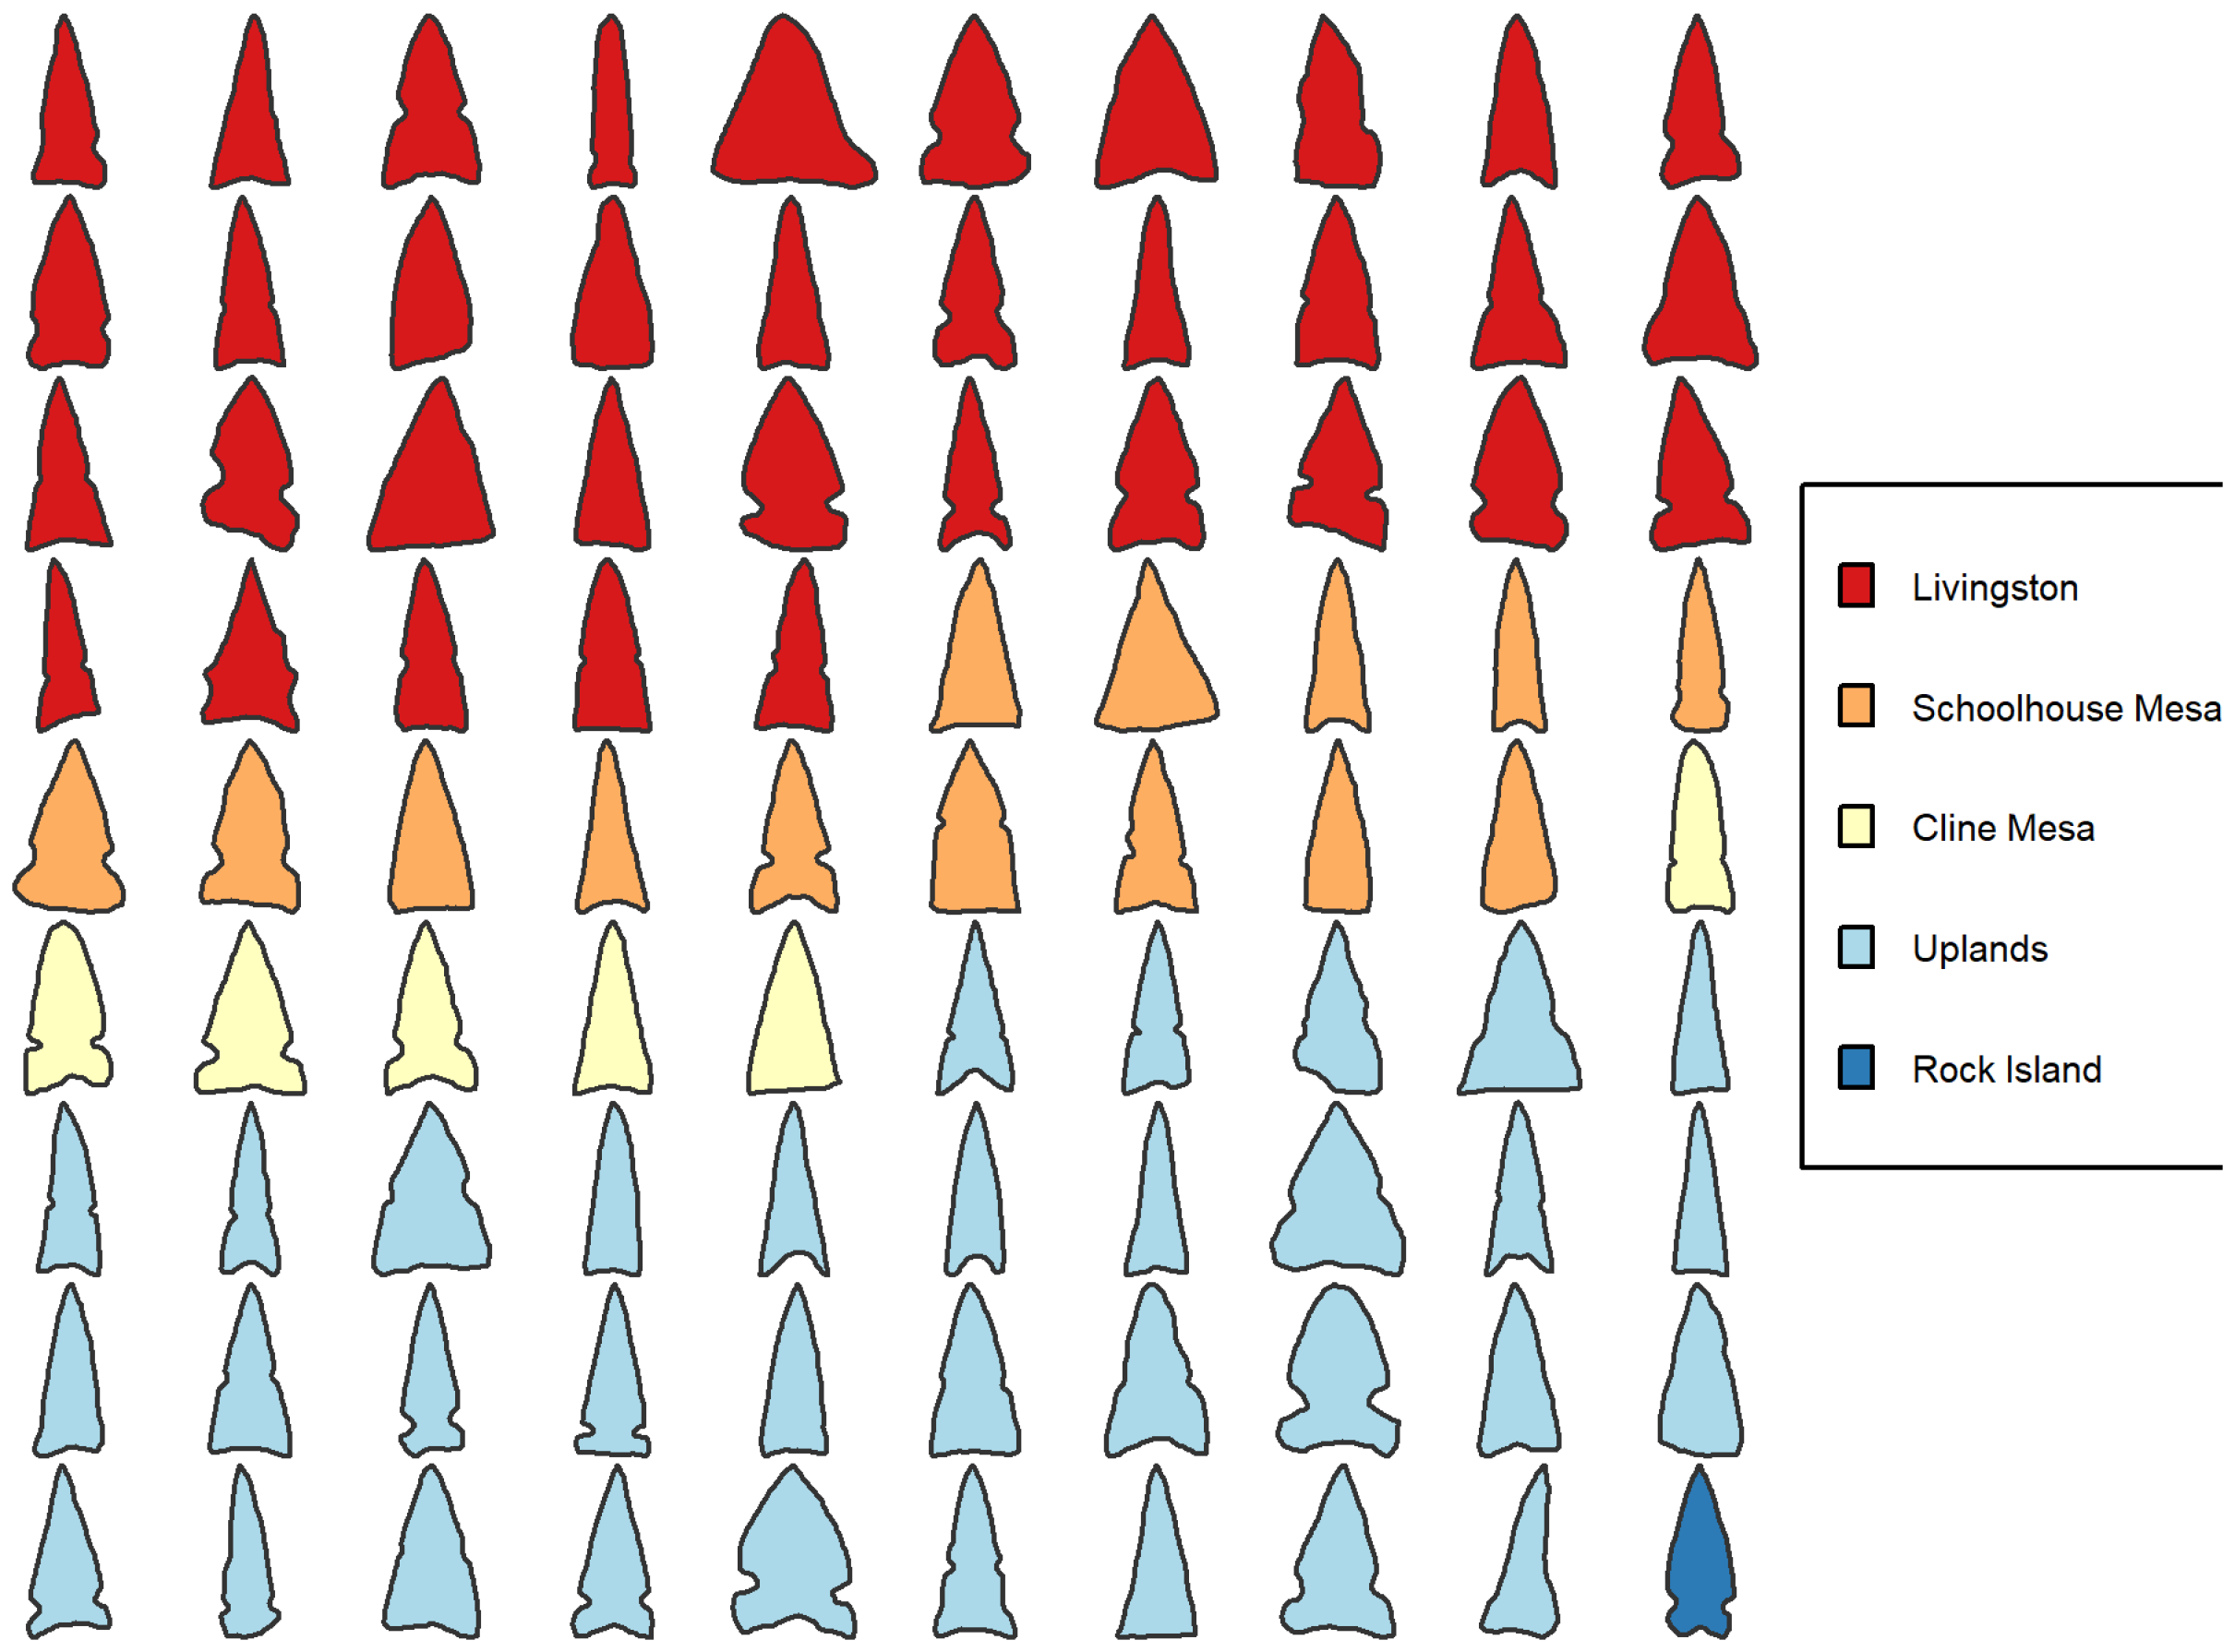
\includegraphics[width=1\linewidth]{figures/TontoPointsFinal} \caption{Outlines of projectile points from sites in the Tonto Basin. Note that the projectile points are not scaled.}\label{fig:TontoPointsFinal}
\end{figure}

\hypertarget{geometric-morphometrics}{%
\subsection{Geometric Morphometrics}\label{geometric-morphometrics}}

I used two GM methods in this analysis: elliptical Fourier analysis
(EFA) and full generalized Procrustes alignment (GPA). Something to keep
in mind is that GM methods analyze the form of the object separated from
size, position, and orientation. Real-world measurements such as length
and width are not explicitly included in these methods, although
relative dimensions, such as length to width ratio are captured in the
overall form of the object. Measurements such as length and weight can
be included in various analyses but are not included here. The purpose
of this study is to determine whether GM methods alone are sufficient to
discriminate between types of projectile points and how they can best be
used in the context of the U.S. Southwest.

EFA was developed by Kuhl and Giardina
(\protect\hyperlink{ref-Kuhl1982-kd}{1982}) as a quantitative means for
describing a closed outline. There are a handful of papers that use EFA
for lithic studies in archaeology (e.g.,
\protect\hyperlink{ref-Cardillo2010-ys}{Cardillo 2010};
\protect\hyperlink{ref-Fox2015-ox}{Fox 2015};
\protect\hyperlink{ref-Gingerich2014-cb}{Gingerich et al. 2014};
\protect\hyperlink{ref-Hoggard2019-yw}{Hoggard, McNabb, and Cole 2019};
\protect\hyperlink{ref-Iovita2011-nz}{Iovita 2011};
\protect\hyperlink{ref-Iovita2011-zp}{Iovita and McPherron 2011}). The
mathematics behind the method are complex to describe, which is one
reason the method has not been adopted as quickly as it should be (see
\protect\hyperlink{ref-Caple2017-mk}{Caple, Byrd, and Stephan 2017}).
Caple and colleagues (\protect\hyperlink{ref-Caple2017-mk}{Caple, Byrd,
and Stephan 2017}) provide an excellent description of EFA for
non-mathematicians, and the reader is referred to their treatise for
more details. For my purposes, it is enough to know that EFA analysis
requires a closed outline and a number of harmonics. The harmonics can
be thought of as ellipses in a time series used to describe the shape of
the object. Three harmonics can be used to create an oval shape, and 12
harmonics is sufficient for a complex projectile point outline. The
number of harmonics necessary to capture the outline can be computed.
For example, if you wish to reconstruct an outline with 99.9\% accuracy,
then the exact number of harmonics necessary can be calculated using the
formula: \[ HarmonicPower_n = \frac{A^2_n+B^2_n+C^2_n+D^2_n}{2} \] where
n is the harmonic power and A, B, C, and D are the coefficients
generated from the EFA. EFA creates a series of coefficients--four for
each harmonic (A,B,C,D)--which can be used in multivariate statistics.
Most commonly, principal components analysis (PCA) is used to transform
the EFA values. The PCA results can then be used in distance-based
methods such as clustering or even network analysis.

Generalized Procrustes Analysis, or GPA, is primarily a way to align,
scale, and rotate points (\protect\hyperlink{ref-Gower1975-uv}{Gower
1975}). Instead of outlines like EFA, GPA requires landmarks located on
homologous locations for each object
(\protect\hyperlink{ref-Rohlf1990-mp}{Rohlf and Slice 1990}). As an
alternative to landmarks, semilandmarks can be placed at equidistant
locations around the object. There is substantial discussion on the
validity of certain types of landmarks and the use of semilandmarks as
landmarks (e.g., \protect\hyperlink{ref-De_Groote2011-mh}{De Groote
2011}; \protect\hyperlink{ref-MacLeod2017-yl}{MacLeod 2017};
\protect\hyperlink{ref-Okumura2019-ur}{Okumura and Araujo 2019};
\protect\hyperlink{ref-Shott2010-fn}{Shott and Trail 2010}). Although
there are some methods that can introduce error, there is no reason to
exclude semi-landmarks outright. One disadvantage of traditional
landmark analysis, compared to EFA, is that the analyst must be more
involved in the selection of the number and placement of landmarks. Once
the landmarks, or semilandmarks are placed on the objects, they are
iteratively modified to achieve the best possible alignment between
shapes without changing the relative positions between landmarks. This
modification is done using the GPA procedure. As with EFA, the next step
is usually to perform a PCA analysis. Landmark analysis using GPA is
more common, so far, in archaeological analysis of stone tools than EFA
(e.g., \protect\hyperlink{ref-Archer2018-zi}{Archer et al. 2018};
\protect\hyperlink{ref-Bischoff2020-zn}{Bischoff and Allison 2020};
\protect\hyperlink{ref-Buchanan2015-dx}{Buchanan et al. 2015};
\protect\hyperlink{ref-Charlin2018-yg}{Charlin and González-José 2018};
\protect\hyperlink{ref-Fisher2018-jq}{Fisher 2018};
\protect\hyperlink{ref-Gingerich2014-cb}{Gingerich et al. 2014};
\protect\hyperlink{ref-Herzlinger2017-ce}{Herzlinger, Goren-Inbar, and
Grosman 2017}; \protect\hyperlink{ref-Lycett2010-od}{Lycett,
Cramon-Taubadel, and Gowlett 2010};
\protect\hyperlink{ref-Riede2019-gb}{Riede, Hoggard, and Shennan 2019};
\protect\hyperlink{ref-Selden2020-ni}{Selden, Dockall, and Dubied 2020};
\protect\hyperlink{ref-Shott2010-fn}{Shott and Trail 2010};
\protect\hyperlink{ref-Smith2015-qk}{Smith, Smallwood, and DeWitt 2015};
\protect\hyperlink{ref-Thulman2012-fo}{Thulman 2012}).

The project was initially designed to compare the EFA results with a
semilandmark analysis using the full outline of the projectile point by
taking a sample of the outline and using the sampled coordinates as
landmarks. Both approaches yielded similar results, but neither achieved
satisfactory accuracy. The research design was then modified to include
a more traditional landmark analysis to determine whether it would
improve upon the initial design.

There are some disadvantages to using landmarks, which is why the
EFA/semilandmark approach was initially favored. The principal
disadvantages to using landmarks are reproducibility and accuracy.
Landmarks are more subjective in many ways than the semilandmarks or EFA
(see \protect\hyperlink{ref-Shott2010-fn}{Shott and Trail 2010, 205}).
The analyst must decide how many points to place, what topological
points should be used as landmarks, and how many landmarks should be
used. The placement of landmarks can vary between analysts and can be
affected by the instruments or software used to collect or create the
landmarks. Another major concern is the loss of detail from not
considering the entire outline. Serrated points and points with more
than one notch (this occurs more often than one might expect in
Southwestern points) are difficult to capture without including a lot of
landmarks, which are only applicable in a minority of situations.
Secondary to these points, but still a concern, is that placing
landmarks can be a more time-consuming process, as it is not as subject
to automation as semilandmarks or EFA.

Despite the disadvantages, landmarks are widely used for good reasons. I
see two main advantages to landmark analysis in the context of
projectile point analysis. The first is that the analyst can use their
prior experience to determine what topological locations on the
projectile point are most useful for discriminating between types.
Decades of research on projectile points has refined many typologies
into useful tools, despite their limitations. This knowledge can be
applied to choosing appropriate landmarks. The second advantage is that
outline analysis requires complete points, whereas landmark analysis can
use damaged points. If chunks of the projectile are missing then the
outline is not usable. Possibly, the missing portion could be estimated
and filled in, but that process is more error prone than estimating
missing landmarks. Landmarks can be placed on reconstructed projectile
point illustrations or missing landmarks can be estimated mathematically
(\protect\hyperlink{ref-Gunz2009-yb}{Gunz et al. 2009}). Most projectile
points suffer from some type of damage and some of the projectile points
I classified as ``complete'' suffer from minor damage to the tip of the
point or elsewhere. The use of damaged points can greatly increase the
available sample size for studies, which is often a major limitation in
projectile point studies.

Landmark configurations can vary significantly, depending on what the
analysis is designed to measure and on the point type. Most of the area
of a projectile point is usually in the blade--the portion above the
notches. The base of the point, the portion below the notches, is also
the hafting element. For projectile point typologies, the base of the
point usually contains the most important elements for determining the
type--notching style and basal shape being the two major elements. Thus,
if most of the landmarks are on the blade margins then the base of the
point is not getting as much coverage. It is more than just tradition
that the base gets the most attention. Hafting a point is an important
technological choice, more so than how long the point is. Furthermore,
projectile points can be resharpened. Resharpening the blade margins can
modify the shape of the blade and change its appearance. While it is
possible to modify the base of the point and even convert a side-notched
point into a corner-notched point and vice-versa, it is unlikely that
this happened regularly with the small arrowpoints used in this study
(\protect\hyperlink{ref-Loendorf2019-df}{Loendorf et al. 2019}).

Because of the vagaries of placing landmarks, I used two configurations
in this study. In the first configuration, the full outline was used.
Only what I term, the corner of the projectile point was used in the
second configuration. Figure 8 shows the first landmark configurations.
The landmark configuration was designed to place fewer landmarks along
the blade margins and more landmarks along the notches and the base.
Separate curves were placed between the tip of the point and the notches
and the notches and the base (or the tip and the base for triangular
points), and landmarks were placed at equidistant locations along the
curves. The second configuration is much sparser (figure 9). The
landmarks were placed only on the right side of the point--this was
arbitrarily chosen. For the side-notched and corner-notched points,
landmarking started from the top of the notch, moved to the middle of
the notch and then the bottom portion of the notch. For corner-notched
points, this last landmark marked the right corner of the point, but for
side-notched points an additional landmark was placed. The final
landmark was placed at the center of the basal margin. Triangular points
differed by placing the first landmark in the center of the blade
margin. The first approach contains between 30 and 42 landmarks that
cover the entire point outline, whereas the second ranges from 3 to 5
landmarks that cover only a portion of the projectile point. These
extremes were chosen to provide significant contrast between approaches.

\begin{figure}
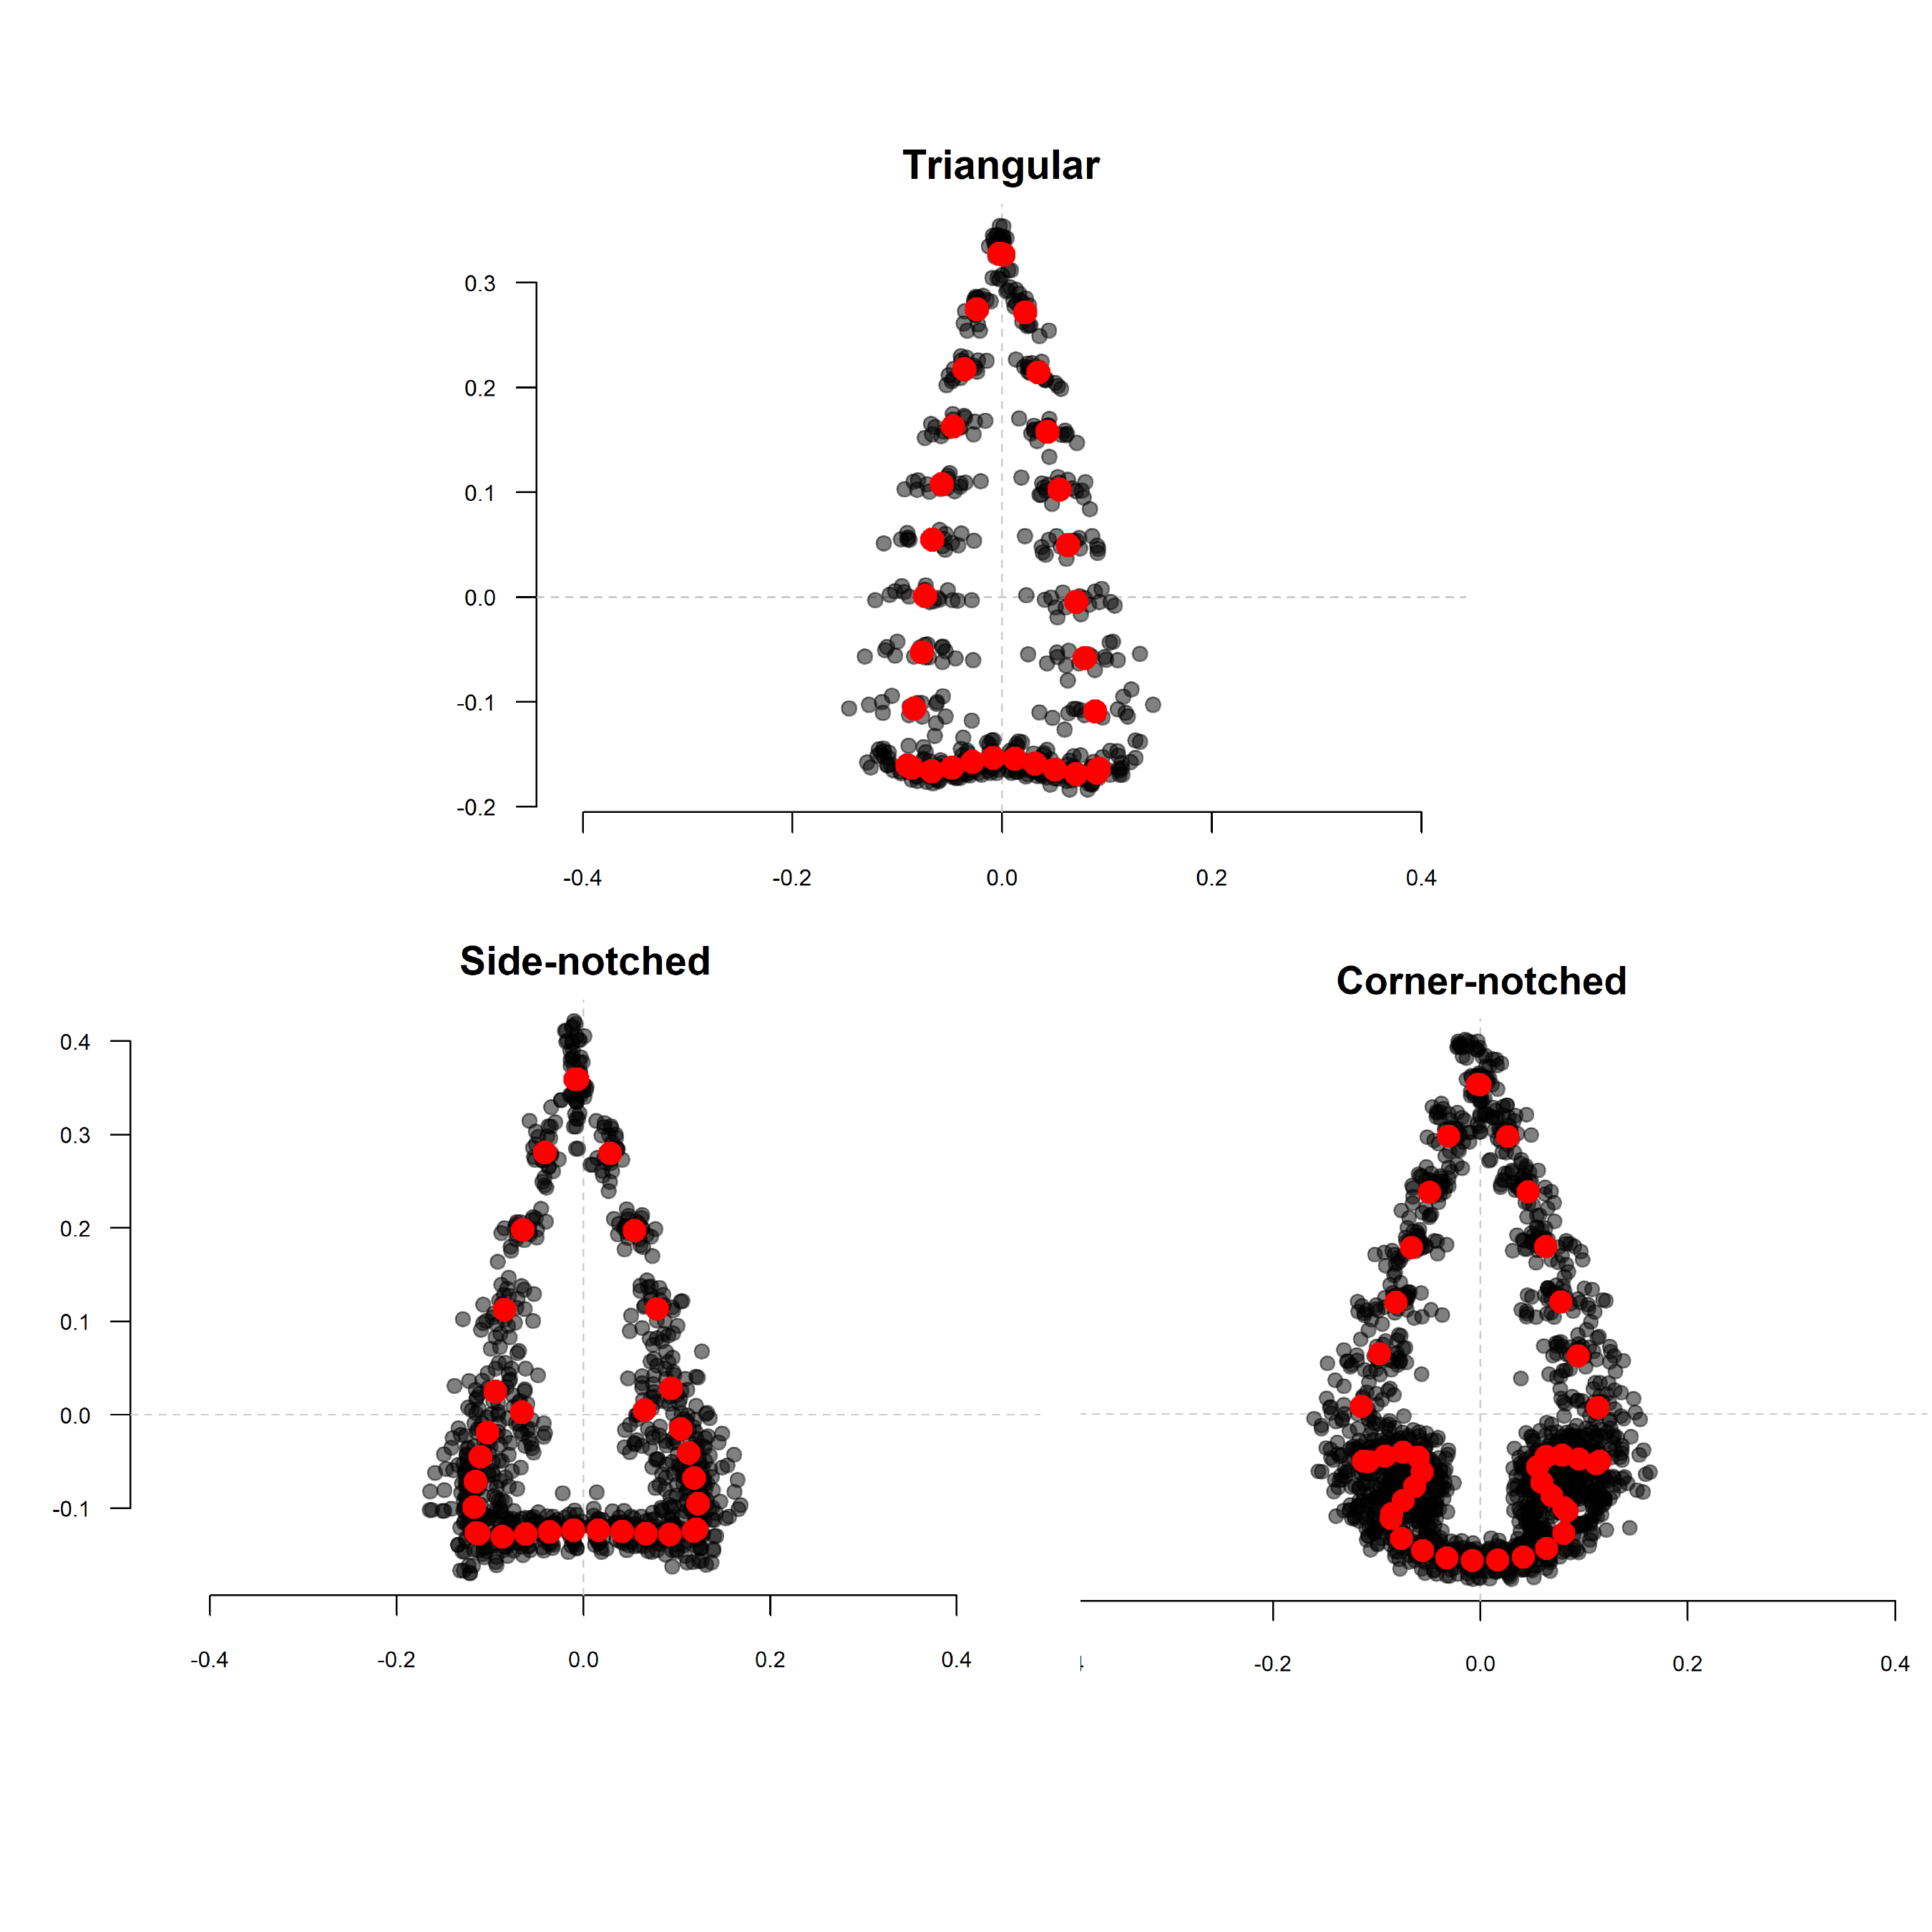
\includegraphics[width=1\linewidth]{figures/curveComparison} \caption{Comparison of the full outline landmarks for corner-notched, side-notched and triangular shaped points from Justice's (2002) projectile point illustrations. Red dots indicate the mean location for each of the landmarks.}\label{fig:curvesStack}
\end{figure}

\begin{figure}
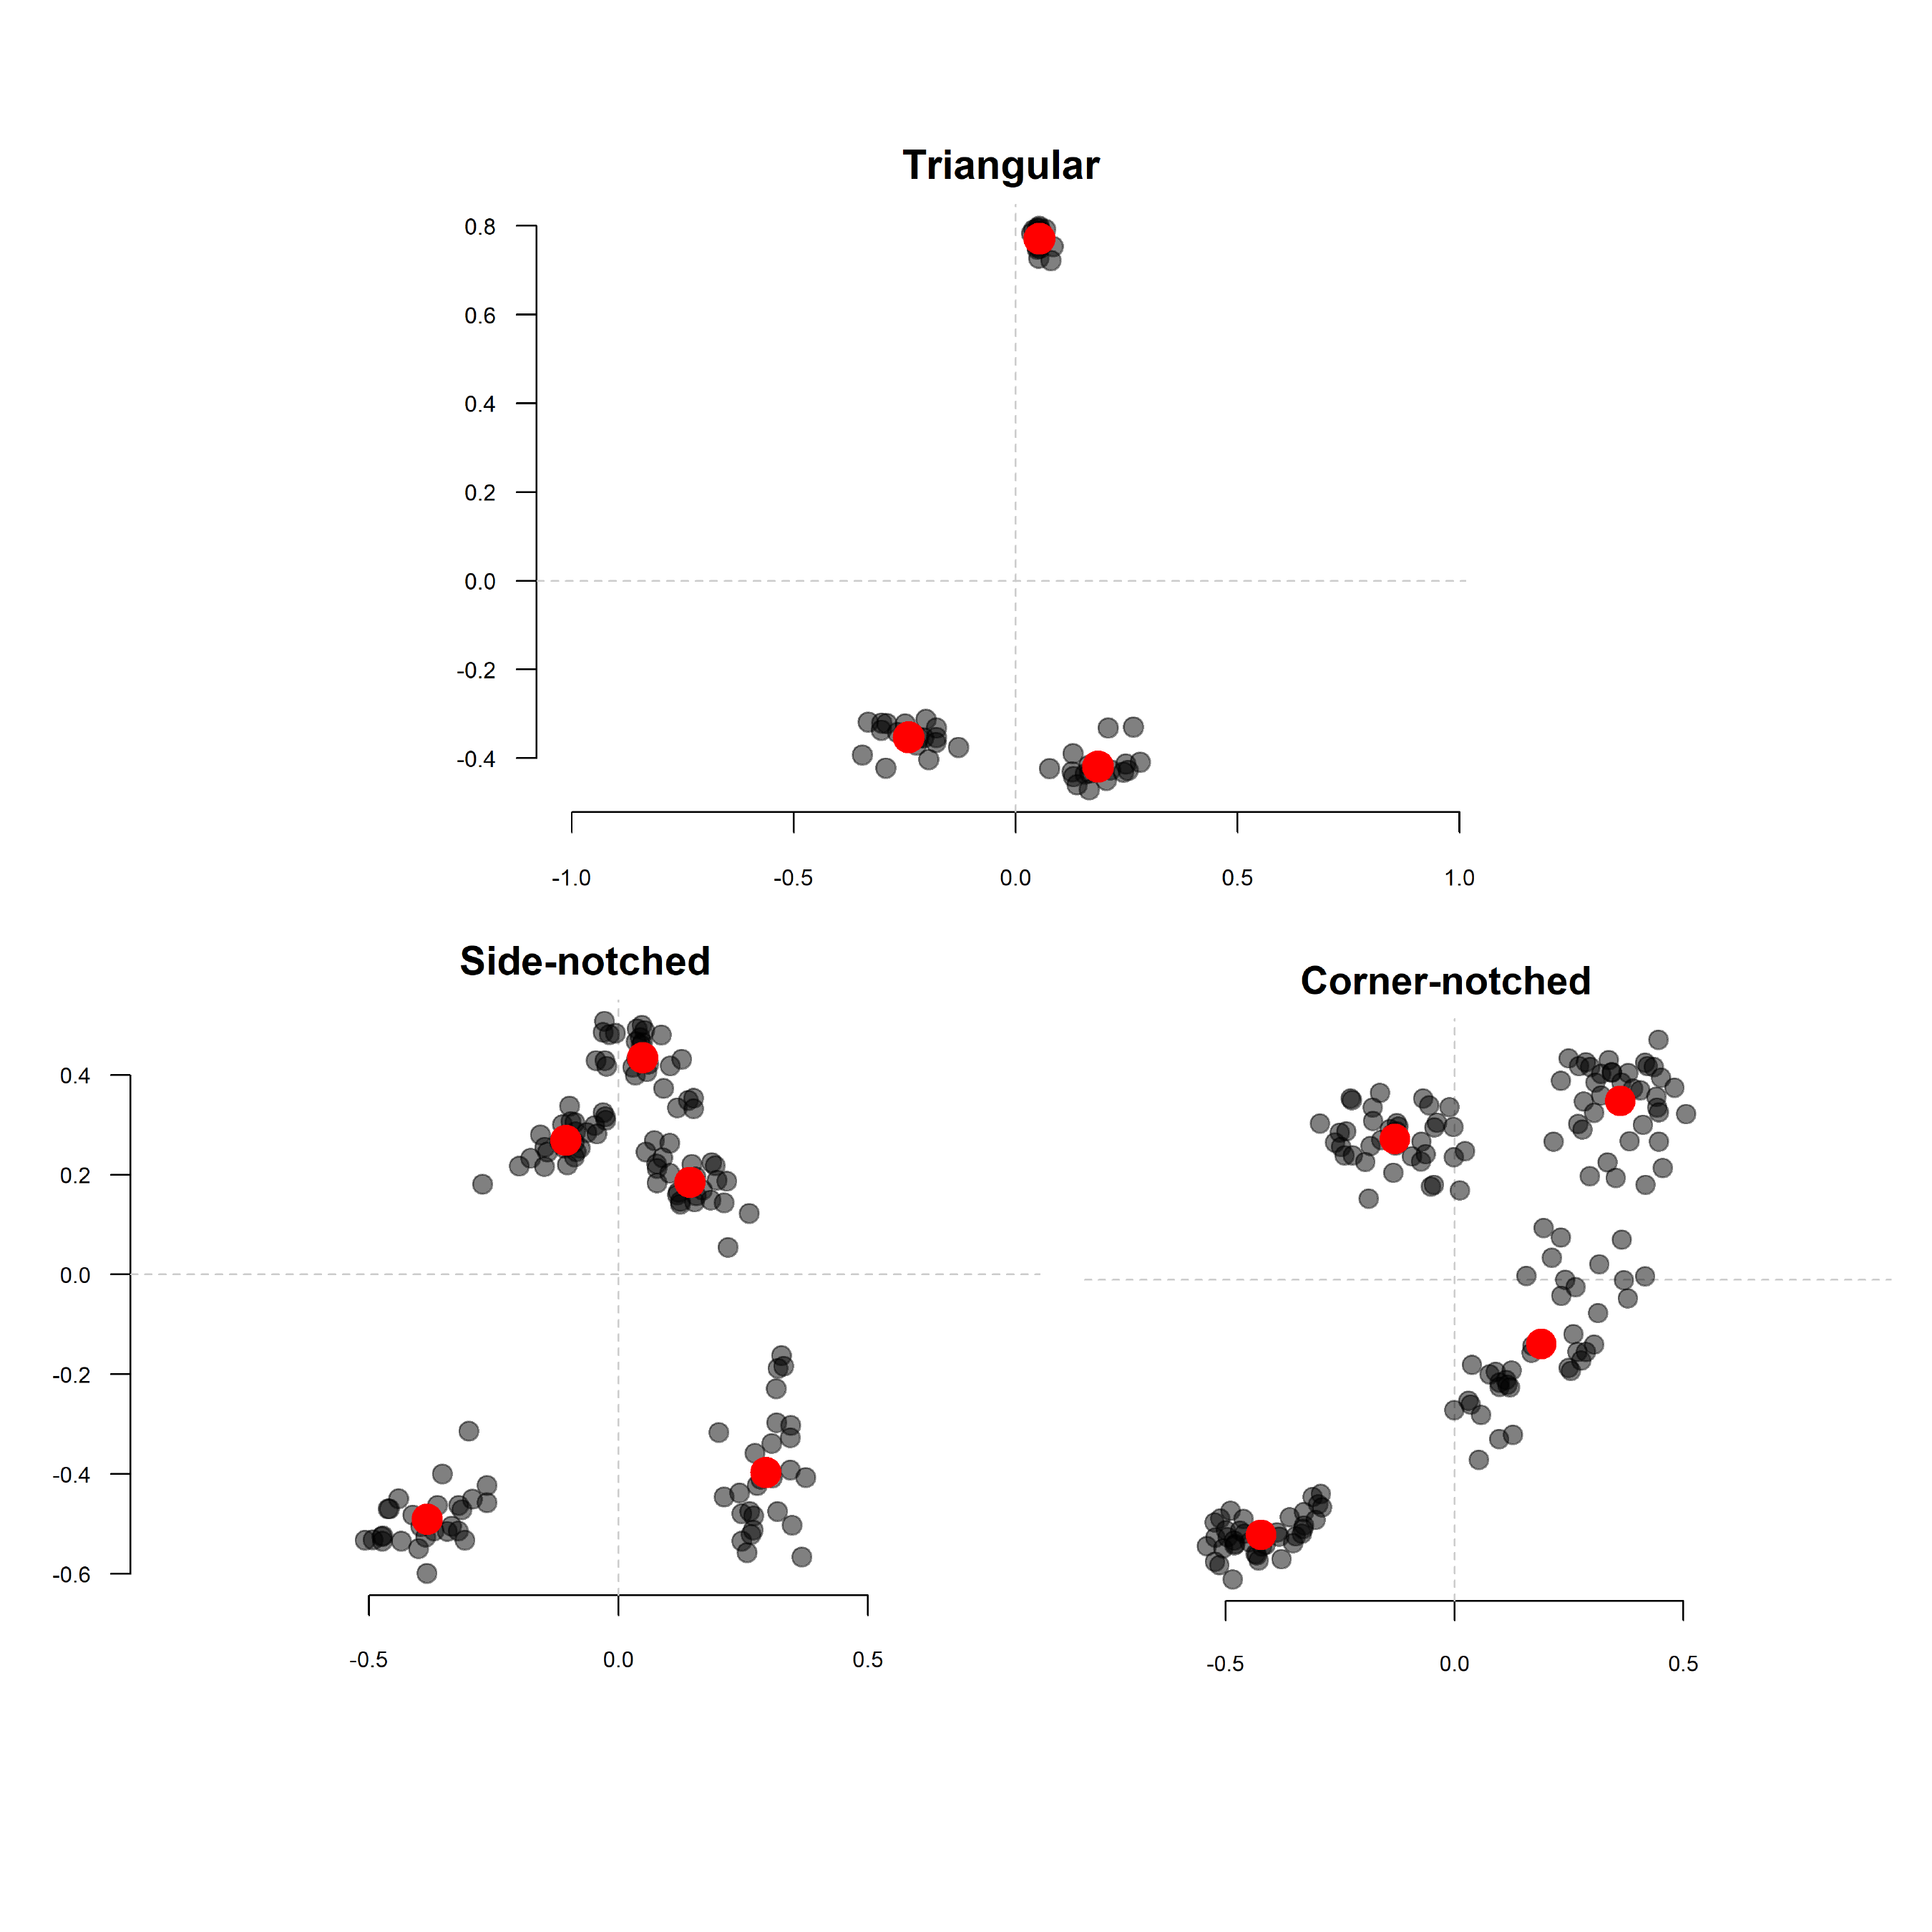
\includegraphics[width=1\linewidth]{figures/cornerComparison} \caption{Comparison of the projectile point corner's landmarks for corner-notched, side-notched and triangular shaped points from Justice's (2002) projectile point illustrations. Red dots indicate the mean location for each of the landmarks.}\label{fig:cornerComparison}
\end{figure}

\hypertarget{comparisons}{%
\section{Comparisons}\label{comparisons}}

The first step in the analysis was to determine how well projectile
points typed by Justice could be correctly assigned using GM methods.
Linear discriminant analysis (LDA) was used to type the projectile
points using the GM results. A general target of 0.85 was arbitrarily
chosen as a minimum target for acceptable results--meaning that 85\% of
the projectile points were classified correctly. As mentioned
previously, Justice placed each projectile point type into a cluster.
Presumably, projectile point types in the same cluster should be more
closely related than they are to projectile point types in other
clusters. This gives another level of comparison that was used in
addition to the types.

The original intent was to compare EFA versus semilandmarks placed at
equidistant locations around the outline. However, these results were
unsatisfactory, and a more traditional landmark analysis was also
completed. Because the number and placement of landmarks has a
significant impact on the outcome of the study, two different landmark
configurations were used.

Part of the reason the results were unsatisfactory for the EFA and
semilandmarks was that the LDA analysis had trouble discriminating
between notched and unnotched points and between side-notched and
corner-notched points. These are some of the most basic distinctions
that are made when analyzing projectile points. While it would be
convenient if the analysis did not require an additional step, it is not
difficult to separate the points into these basic shapes prior to the GM
analysis. I separated the Justice points into three classes:
side-notched, corner-notched, and triangular. For this study, I combined
stemmed points into the corner-notched category.

Tables 2, 3, and 4 show the LDA results by type, cluster, and by shape.
These tables will be referred to in the sections that follow.

 
  \providecommand{\huxb}[2]{\arrayrulecolor[RGB]{#1}\global\arrayrulewidth=#2pt}
  \providecommand{\huxvb}[2]{\color[RGB]{#1}\vrule width #2pt}
  \providecommand{\huxtpad}[1]{\rule{0pt}{#1}}
  \providecommand{\huxbpad}[1]{\rule[-#1]{0pt}{#1}}

\begin{table}[ht]
\begin{centerbox}
\begin{threeparttable}
\captionsetup{justification=centering,singlelinecheck=off}
\caption{Linear Discriminant Analysis Results for Projectile Point Types}
 \label{tab:LDAResultsType}
\setlength{\tabcolsep}{0pt}
\begin{tabular}{l l l l l l}


\hhline{}
\arrayrulecolor{black}

\multicolumn{1}{!{\huxvb{0, 0, 0}{0}}l!{\huxvb{0, 0, 0}{0}}}{\huxtpad{1pt + 1em}\raggedright \hspace{0pt} \textbf{Type} \hspace{1pt}\huxbpad{1pt}} &
\multicolumn{1}{r!{\huxvb{0, 0, 0}{0}}}{\huxtpad{1pt + 1em}\raggedleft \hspace{1pt} \textbf{EFA} \hspace{1pt}\huxbpad{1pt}} &
\multicolumn{1}{r!{\huxvb{0, 0, 0}{0}}}{\huxtpad{1pt + 1em}\raggedleft \hspace{1pt} \textbf{semiLdk} \hspace{1pt}\huxbpad{1pt}} &
\multicolumn{1}{r!{\huxvb{0, 0, 0}{0}}}{\huxtpad{1pt + 1em}\raggedleft \hspace{1pt} \textbf{Ldk} \hspace{1pt}\huxbpad{1pt}} &
\multicolumn{1}{r!{\huxvb{0, 0, 0}{0}}}{\huxtpad{1pt + 1em}\raggedleft \hspace{1pt} \textbf{Ldk-corner} \hspace{1pt}\huxbpad{1pt}} &
\multicolumn{1}{r!{\huxvb{0, 0, 0}{0}}}{\huxtpad{1pt + 1em}\raggedleft \hspace{1pt} \textbf{Mean} \hspace{0pt}\huxbpad{1pt}} \tabularnewline[-0.5pt]


\hhline{>{\huxb{0, 0, 0}{0.4}}->{\huxb{0, 0, 0}{0.4}}->{\huxb{0, 0, 0}{0.4}}->{\huxb{0, 0, 0}{0.4}}->{\huxb{0, 0, 0}{0.4}}->{\huxb{0, 0, 0}{0.4}}-}
\arrayrulecolor{black}

\multicolumn{1}{!{\huxvb{0, 0, 0}{0}}l!{\huxvb{0, 0, 0}{0}}}{\huxtpad{1pt + 1em}\raggedright \hspace{0pt} Chaco Corner Notched \hspace{1pt}\huxbpad{1pt}} &
\multicolumn{1}{r!{\huxvb{0, 0, 0}{0}}}{\huxtpad{1pt + 1em}\raggedleft \hspace{1pt} 0.56 \hspace{1pt}\huxbpad{1pt}} &
\multicolumn{1}{r!{\huxvb{0, 0, 0}{0}}}{\huxtpad{1pt + 1em}\raggedleft \hspace{1pt} 0.89 \hspace{1pt}\huxbpad{1pt}} &
\multicolumn{1}{r!{\huxvb{0, 0, 0}{0}}}{\huxtpad{1pt + 1em}\raggedleft \hspace{1pt} 0.85 \hspace{1pt}\huxbpad{1pt}} &
\multicolumn{1}{r!{\huxvb{0, 0, 0}{0}}}{\huxtpad{1pt + 1em}\raggedleft \hspace{1pt} 0.85 \hspace{1pt}\huxbpad{1pt}} &
\multicolumn{1}{r!{\huxvb{0, 0, 0}{0}}}{\huxtpad{1pt + 1em}\raggedleft \hspace{1pt} 0.79 \hspace{0pt}\huxbpad{1pt}} \tabularnewline[-0.5pt]


\hhline{}
\arrayrulecolor{black}

\multicolumn{1}{!{\huxvb{0, 0, 0}{0}}l!{\huxvb{0, 0, 0}{0}}}{\huxtpad{1pt + 1em}\raggedright \hspace{0pt} Cottonwood Triangular \hspace{1pt}\huxbpad{1pt}} &
\multicolumn{1}{r!{\huxvb{0, 0, 0}{0}}}{\huxtpad{1pt + 1em}\raggedleft \hspace{1pt} 0.38 \hspace{1pt}\huxbpad{1pt}} &
\multicolumn{1}{r!{\huxvb{0, 0, 0}{0}}}{\huxtpad{1pt + 1em}\raggedleft \hspace{1pt} 0.38 \hspace{1pt}\huxbpad{1pt}} &
\multicolumn{1}{r!{\huxvb{0, 0, 0}{0}}}{\huxtpad{1pt + 1em}\raggedleft \hspace{1pt} 1\hphantom{0}\hphantom{0}\hphantom{0} \hspace{1pt}\huxbpad{1pt}} &
\multicolumn{1}{r!{\huxvb{0, 0, 0}{0}}}{\huxtpad{1pt + 1em}\raggedleft \hspace{1pt} 0.75 \hspace{1pt}\huxbpad{1pt}} &
\multicolumn{1}{r!{\huxvb{0, 0, 0}{0}}}{\huxtpad{1pt + 1em}\raggedleft \hspace{1pt} 0.63 \hspace{0pt}\huxbpad{1pt}} \tabularnewline[-0.5pt]


\hhline{}
\arrayrulecolor{black}

\multicolumn{1}{!{\huxvb{0, 0, 0}{0}}l!{\huxvb{0, 0, 0}{0}}}{\huxtpad{1pt + 1em}\raggedright \hspace{0pt} Guadalupe \hspace{1pt}\huxbpad{1pt}} &
\multicolumn{1}{r!{\huxvb{0, 0, 0}{0}}}{\huxtpad{1pt + 1em}\raggedleft \hspace{1pt} 0.75 \hspace{1pt}\huxbpad{1pt}} &
\multicolumn{1}{r!{\huxvb{0, 0, 0}{0}}}{\huxtpad{1pt + 1em}\raggedleft \hspace{1pt} 0.83 \hspace{1pt}\huxbpad{1pt}} &
\multicolumn{1}{r!{\huxvb{0, 0, 0}{0}}}{\huxtpad{1pt + 1em}\raggedleft \hspace{1pt} 0.93 \hspace{1pt}\huxbpad{1pt}} &
\multicolumn{1}{r!{\huxvb{0, 0, 0}{0}}}{\huxtpad{1pt + 1em}\raggedleft \hspace{1pt} 0.93 \hspace{1pt}\huxbpad{1pt}} &
\multicolumn{1}{r!{\huxvb{0, 0, 0}{0}}}{\huxtpad{1pt + 1em}\raggedleft \hspace{1pt} 0.86 \hspace{0pt}\huxbpad{1pt}} \tabularnewline[-0.5pt]


\hhline{}
\arrayrulecolor{black}

\multicolumn{1}{!{\huxvb{0, 0, 0}{0}}l!{\huxvb{0, 0, 0}{0}}}{\huxtpad{1pt + 1em}\raggedright \hspace{0pt} Pueblo Alto Side Notched \hspace{1pt}\huxbpad{1pt}} &
\multicolumn{1}{r!{\huxvb{0, 0, 0}{0}}}{\huxtpad{1pt + 1em}\raggedleft \hspace{1pt} 0.86 \hspace{1pt}\huxbpad{1pt}} &
\multicolumn{1}{r!{\huxvb{0, 0, 0}{0}}}{\huxtpad{1pt + 1em}\raggedleft \hspace{1pt} 0.71 \hspace{1pt}\huxbpad{1pt}} &
\multicolumn{1}{r!{\huxvb{0, 0, 0}{0}}}{\huxtpad{1pt + 1em}\raggedleft \hspace{1pt} 1\hphantom{0}\hphantom{0}\hphantom{0} \hspace{1pt}\huxbpad{1pt}} &
\multicolumn{1}{r!{\huxvb{0, 0, 0}{0}}}{\huxtpad{1pt + 1em}\raggedleft \hspace{1pt} 1\hphantom{0}\hphantom{0}\hphantom{0} \hspace{1pt}\huxbpad{1pt}} &
\multicolumn{1}{r!{\huxvb{0, 0, 0}{0}}}{\huxtpad{1pt + 1em}\raggedleft \hspace{1pt} 0.89 \hspace{0pt}\huxbpad{1pt}} \tabularnewline[-0.5pt]


\hhline{}
\arrayrulecolor{black}

\multicolumn{1}{!{\huxvb{0, 0, 0}{0}}l!{\huxvb{0, 0, 0}{0}}}{\huxtpad{1pt + 1em}\raggedright \hspace{0pt} Pueblo Side Notched Concave Base \hspace{1pt}\huxbpad{1pt}} &
\multicolumn{1}{r!{\huxvb{0, 0, 0}{0}}}{\huxtpad{1pt + 1em}\raggedleft \hspace{1pt} 0.44 \hspace{1pt}\huxbpad{1pt}} &
\multicolumn{1}{r!{\huxvb{0, 0, 0}{0}}}{\huxtpad{1pt + 1em}\raggedleft \hspace{1pt} 0.78 \hspace{1pt}\huxbpad{1pt}} &
\multicolumn{1}{r!{\huxvb{0, 0, 0}{0}}}{\huxtpad{1pt + 1em}\raggedleft \hspace{1pt} 0.73 \hspace{1pt}\huxbpad{1pt}} &
\multicolumn{1}{r!{\huxvb{0, 0, 0}{0}}}{\huxtpad{1pt + 1em}\raggedleft \hspace{1pt} 0.73 \hspace{1pt}\huxbpad{1pt}} &
\multicolumn{1}{r!{\huxvb{0, 0, 0}{0}}}{\huxtpad{1pt + 1em}\raggedleft \hspace{1pt} 0.67 \hspace{0pt}\huxbpad{1pt}} \tabularnewline[-0.5pt]


\hhline{}
\arrayrulecolor{black}

\multicolumn{1}{!{\huxvb{0, 0, 0}{0}}l!{\huxvb{0, 0, 0}{0}}}{\huxtpad{1pt + 1em}\raggedright \hspace{0pt} Pueblo Side Notched Straight Base \hspace{1pt}\huxbpad{1pt}} &
\multicolumn{1}{r!{\huxvb{0, 0, 0}{0}}}{\huxtpad{1pt + 1em}\raggedleft \hspace{1pt} 0.57 \hspace{1pt}\huxbpad{1pt}} &
\multicolumn{1}{r!{\huxvb{0, 0, 0}{0}}}{\huxtpad{1pt + 1em}\raggedleft \hspace{1pt} 0.57 \hspace{1pt}\huxbpad{1pt}} &
\multicolumn{1}{r!{\huxvb{0, 0, 0}{0}}}{\huxtpad{1pt + 1em}\raggedleft \hspace{1pt} 0.43 \hspace{1pt}\huxbpad{1pt}} &
\multicolumn{1}{r!{\huxvb{0, 0, 0}{0}}}{\huxtpad{1pt + 1em}\raggedleft \hspace{1pt} 0.71 \hspace{1pt}\huxbpad{1pt}} &
\multicolumn{1}{r!{\huxvb{0, 0, 0}{0}}}{\huxtpad{1pt + 1em}\raggedleft \hspace{1pt} 0.57 \hspace{0pt}\huxbpad{1pt}} \tabularnewline[-0.5pt]


\hhline{}
\arrayrulecolor{black}

\multicolumn{1}{!{\huxvb{0, 0, 0}{0}}l!{\huxvb{0, 0, 0}{0}}}{\huxtpad{1pt + 1em}\raggedright \hspace{0pt} Snaketown Triangular Concave Base \hspace{1pt}\huxbpad{1pt}} &
\multicolumn{1}{r!{\huxvb{0, 0, 0}{0}}}{\huxtpad{1pt + 1em}\raggedleft \hspace{1pt} 0.78 \hspace{1pt}\huxbpad{1pt}} &
\multicolumn{1}{r!{\huxvb{0, 0, 0}{0}}}{\huxtpad{1pt + 1em}\raggedleft \hspace{1pt} 0.89 \hspace{1pt}\huxbpad{1pt}} &
\multicolumn{1}{r!{\huxvb{0, 0, 0}{0}}}{\huxtpad{1pt + 1em}\raggedleft \hspace{1pt} 0.78 \hspace{1pt}\huxbpad{1pt}} &
\multicolumn{1}{r!{\huxvb{0, 0, 0}{0}}}{\huxtpad{1pt + 1em}\raggedleft \hspace{1pt} 0.89 \hspace{1pt}\huxbpad{1pt}} &
\multicolumn{1}{r!{\huxvb{0, 0, 0}{0}}}{\huxtpad{1pt + 1em}\raggedleft \hspace{1pt} 0.84 \hspace{0pt}\huxbpad{1pt}} \tabularnewline[-0.5pt]


\hhline{}
\arrayrulecolor{black}

\multicolumn{1}{!{\huxvb{0, 0, 0}{0}}l!{\huxvb{0, 0, 0}{0}}}{\huxtpad{1pt + 1em}\raggedright \hspace{0pt} Tularosa Corner Notched \hspace{1pt}\huxbpad{1pt}} &
\multicolumn{1}{r!{\huxvb{0, 0, 0}{0}}}{\huxtpad{1pt + 1em}\raggedleft \hspace{1pt} 0.77 \hspace{1pt}\huxbpad{1pt}} &
\multicolumn{1}{r!{\huxvb{0, 0, 0}{0}}}{\huxtpad{1pt + 1em}\raggedleft \hspace{1pt} 0.69 \hspace{1pt}\huxbpad{1pt}} &
\multicolumn{1}{r!{\huxvb{0, 0, 0}{0}}}{\huxtpad{1pt + 1em}\raggedleft \hspace{1pt} 0.6\hphantom{0} \hspace{1pt}\huxbpad{1pt}} &
\multicolumn{1}{r!{\huxvb{0, 0, 0}{0}}}{\huxtpad{1pt + 1em}\raggedleft \hspace{1pt} 0.8\hphantom{0} \hspace{1pt}\huxbpad{1pt}} &
\multicolumn{1}{r!{\huxvb{0, 0, 0}{0}}}{\huxtpad{1pt + 1em}\raggedleft \hspace{1pt} 0.72 \hspace{0pt}\huxbpad{1pt}} \tabularnewline[-0.5pt]


\hhline{}
\arrayrulecolor{black}

\multicolumn{1}{!{\huxvb{0, 0, 0}{0}}l!{\huxvb{0, 0, 0}{0}}}{\huxtpad{1pt + 1em}\raggedright \hspace{0pt} Mean \hspace{1pt}\huxbpad{1pt}} &
\multicolumn{1}{r!{\huxvb{0, 0, 0}{0}}}{\huxtpad{1pt + 1em}\raggedleft \hspace{1pt} 0.64 \hspace{1pt}\huxbpad{1pt}} &
\multicolumn{1}{r!{\huxvb{0, 0, 0}{0}}}{\huxtpad{1pt + 1em}\raggedleft \hspace{1pt} 0.72 \hspace{1pt}\huxbpad{1pt}} &
\multicolumn{1}{r!{\huxvb{0, 0, 0}{0}}}{\huxtpad{1pt + 1em}\raggedleft \hspace{1pt} 0.79 \hspace{1pt}\huxbpad{1pt}} &
\multicolumn{1}{r!{\huxvb{0, 0, 0}{0}}}{\huxtpad{1pt + 1em}\raggedleft \hspace{1pt} 0.83 \hspace{1pt}\huxbpad{1pt}} &
\multicolumn{1}{r!{\huxvb{0, 0, 0}{0}}}{\huxtpad{1pt + 1em}\raggedleft \hspace{1pt} 0.74 \hspace{0pt}\huxbpad{1pt}} \tabularnewline[-0.5pt]


\hhline{}
\arrayrulecolor{black}
\end{tabular}
\end{threeparttable}\par\end{centerbox}

\end{table}
 

 
  \providecommand{\huxb}[2]{\arrayrulecolor[RGB]{#1}\global\arrayrulewidth=#2pt}
  \providecommand{\huxvb}[2]{\color[RGB]{#1}\vrule width #2pt}
  \providecommand{\huxtpad}[1]{\rule{0pt}{#1}}
  \providecommand{\huxbpad}[1]{\rule[-#1]{0pt}{#1}}

\begin{table}[ht]
\begin{centerbox}
\begin{threeparttable}
\captionsetup{justification=centering,singlelinecheck=off}
\caption{Linear Discriminant Analysis Results for Projectile Point Clusters}
 \label{tab:LDAResultsCluster}
\setlength{\tabcolsep}{0pt}
\begin{tabular}{l l l l l l}


\hhline{}
\arrayrulecolor{black}

\multicolumn{1}{!{\huxvb{0, 0, 0}{0}}l!{\huxvb{0, 0, 0}{0}}}{\huxtpad{1pt + 1em}\raggedright \hspace{0pt} \textbf{Cluster} \hspace{1pt}\huxbpad{1pt}} &
\multicolumn{1}{r!{\huxvb{0, 0, 0}{0}}}{\huxtpad{1pt + 1em}\raggedleft \hspace{1pt} \textbf{EFA} \hspace{1pt}\huxbpad{1pt}} &
\multicolumn{1}{r!{\huxvb{0, 0, 0}{0}}}{\huxtpad{1pt + 1em}\raggedleft \hspace{1pt} \textbf{semiLdk} \hspace{1pt}\huxbpad{1pt}} &
\multicolumn{1}{r!{\huxvb{0, 0, 0}{0}}}{\huxtpad{1pt + 1em}\raggedleft \hspace{1pt} \textbf{Ldk} \hspace{1pt}\huxbpad{1pt}} &
\multicolumn{1}{r!{\huxvb{0, 0, 0}{0}}}{\huxtpad{1pt + 1em}\raggedleft \hspace{1pt} \textbf{Ldk-corner} \hspace{1pt}\huxbpad{1pt}} &
\multicolumn{1}{r!{\huxvb{0, 0, 0}{0}}}{\huxtpad{1pt + 1em}\raggedleft \hspace{1pt} \textbf{Mean} \hspace{0pt}\huxbpad{1pt}} \tabularnewline[-0.5pt]


\hhline{>{\huxb{0, 0, 0}{0.4}}->{\huxb{0, 0, 0}{0.4}}->{\huxb{0, 0, 0}{0.4}}->{\huxb{0, 0, 0}{0.4}}->{\huxb{0, 0, 0}{0.4}}->{\huxb{0, 0, 0}{0.4}}-}
\arrayrulecolor{black}

\multicolumn{1}{!{\huxvb{0, 0, 0}{0}}l!{\huxvb{0, 0, 0}{0}}}{\huxtpad{1pt + 1em}\raggedright \hspace{0pt} Chaco \hspace{1pt}\huxbpad{1pt}} &
\multicolumn{1}{r!{\huxvb{0, 0, 0}{0}}}{\huxtpad{1pt + 1em}\raggedleft \hspace{1pt} 0.81 \hspace{1pt}\huxbpad{1pt}} &
\multicolumn{1}{r!{\huxvb{0, 0, 0}{0}}}{\huxtpad{1pt + 1em}\raggedleft \hspace{1pt} 0.88 \hspace{1pt}\huxbpad{1pt}} &
\multicolumn{1}{r!{\huxvb{0, 0, 0}{0}}}{\huxtpad{1pt + 1em}\raggedleft \hspace{1pt} 0.92 \hspace{1pt}\huxbpad{1pt}} &
\multicolumn{1}{r!{\huxvb{0, 0, 0}{0}}}{\huxtpad{1pt + 1em}\raggedleft \hspace{1pt} 0.92 \hspace{1pt}\huxbpad{1pt}} &
\multicolumn{1}{r!{\huxvb{0, 0, 0}{0}}}{\huxtpad{1pt + 1em}\raggedleft \hspace{1pt} 0.88 \hspace{0pt}\huxbpad{1pt}} \tabularnewline[-0.5pt]


\hhline{}
\arrayrulecolor{black}

\multicolumn{1}{!{\huxvb{0, 0, 0}{0}}l!{\huxvb{0, 0, 0}{0}}}{\huxtpad{1pt + 1em}\raggedright \hspace{0pt} Cienega \hspace{1pt}\huxbpad{1pt}} &
\multicolumn{1}{r!{\huxvb{0, 0, 0}{0}}}{\huxtpad{1pt + 1em}\raggedleft \hspace{1pt} 0.69 \hspace{1pt}\huxbpad{1pt}} &
\multicolumn{1}{r!{\huxvb{0, 0, 0}{0}}}{\huxtpad{1pt + 1em}\raggedleft \hspace{1pt} 0.69 \hspace{1pt}\huxbpad{1pt}} &
\multicolumn{1}{r!{\huxvb{0, 0, 0}{0}}}{\huxtpad{1pt + 1em}\raggedleft \hspace{1pt} 0.6\hphantom{0} \hspace{1pt}\huxbpad{1pt}} &
\multicolumn{1}{r!{\huxvb{0, 0, 0}{0}}}{\huxtpad{1pt + 1em}\raggedleft \hspace{1pt} 0.8\hphantom{0} \hspace{1pt}\huxbpad{1pt}} &
\multicolumn{1}{r!{\huxvb{0, 0, 0}{0}}}{\huxtpad{1pt + 1em}\raggedleft \hspace{1pt} 0.7\hphantom{0} \hspace{0pt}\huxbpad{1pt}} \tabularnewline[-0.5pt]


\hhline{}
\arrayrulecolor{black}

\multicolumn{1}{!{\huxvb{0, 0, 0}{0}}l!{\huxvb{0, 0, 0}{0}}}{\huxtpad{1pt + 1em}\raggedright \hspace{0pt} Livermore \hspace{1pt}\huxbpad{1pt}} &
\multicolumn{1}{r!{\huxvb{0, 0, 0}{0}}}{\huxtpad{1pt + 1em}\raggedleft \hspace{1pt} 0.83 \hspace{1pt}\huxbpad{1pt}} &
\multicolumn{1}{r!{\huxvb{0, 0, 0}{0}}}{\huxtpad{1pt + 1em}\raggedleft \hspace{1pt} 0.75 \hspace{1pt}\huxbpad{1pt}} &
\multicolumn{1}{r!{\huxvb{0, 0, 0}{0}}}{\huxtpad{1pt + 1em}\raggedleft \hspace{1pt} 0.93 \hspace{1pt}\huxbpad{1pt}} &
\multicolumn{1}{r!{\huxvb{0, 0, 0}{0}}}{\huxtpad{1pt + 1em}\raggedleft \hspace{1pt} 0.93 \hspace{1pt}\huxbpad{1pt}} &
\multicolumn{1}{r!{\huxvb{0, 0, 0}{0}}}{\huxtpad{1pt + 1em}\raggedleft \hspace{1pt} 0.86 \hspace{0pt}\huxbpad{1pt}} \tabularnewline[-0.5pt]


\hhline{}
\arrayrulecolor{black}

\multicolumn{1}{!{\huxvb{0, 0, 0}{0}}l!{\huxvb{0, 0, 0}{0}}}{\huxtpad{1pt + 1em}\raggedright \hspace{0pt} Pueblo Side Notched \hspace{1pt}\huxbpad{1pt}} &
\multicolumn{1}{r!{\huxvb{0, 0, 0}{0}}}{\huxtpad{1pt + 1em}\raggedleft \hspace{1pt} 0.75 \hspace{1pt}\huxbpad{1pt}} &
\multicolumn{1}{r!{\huxvb{0, 0, 0}{0}}}{\huxtpad{1pt + 1em}\raggedleft \hspace{1pt} 0.56 \hspace{1pt}\huxbpad{1pt}} &
\multicolumn{1}{r!{\huxvb{0, 0, 0}{0}}}{\huxtpad{1pt + 1em}\raggedleft \hspace{1pt} 0.89 \hspace{1pt}\huxbpad{1pt}} &
\multicolumn{1}{r!{\huxvb{0, 0, 0}{0}}}{\huxtpad{1pt + 1em}\raggedleft \hspace{1pt} 1\hphantom{0}\hphantom{0}\hphantom{0} \hspace{1pt}\huxbpad{1pt}} &
\multicolumn{1}{r!{\huxvb{0, 0, 0}{0}}}{\huxtpad{1pt + 1em}\raggedleft \hspace{1pt} 0.8\hphantom{0} \hspace{0pt}\huxbpad{1pt}} \tabularnewline[-0.5pt]


\hhline{}
\arrayrulecolor{black}

\multicolumn{1}{!{\huxvb{0, 0, 0}{0}}l!{\huxvb{0, 0, 0}{0}}}{\huxtpad{1pt + 1em}\raggedright \hspace{0pt} Snaketown \hspace{1pt}\huxbpad{1pt}} &
\multicolumn{1}{r!{\huxvb{0, 0, 0}{0}}}{\huxtpad{1pt + 1em}\raggedleft \hspace{1pt} 0.78 \hspace{1pt}\huxbpad{1pt}} &
\multicolumn{1}{r!{\huxvb{0, 0, 0}{0}}}{\huxtpad{1pt + 1em}\raggedleft \hspace{1pt} 0.89 \hspace{1pt}\huxbpad{1pt}} &
\multicolumn{1}{r!{\huxvb{0, 0, 0}{0}}}{\huxtpad{1pt + 1em}\raggedleft \hspace{1pt} 0.78 \hspace{1pt}\huxbpad{1pt}} &
\multicolumn{1}{r!{\huxvb{0, 0, 0}{0}}}{\huxtpad{1pt + 1em}\raggedleft \hspace{1pt} 0.89 \hspace{1pt}\huxbpad{1pt}} &
\multicolumn{1}{r!{\huxvb{0, 0, 0}{0}}}{\huxtpad{1pt + 1em}\raggedleft \hspace{1pt} 0.84 \hspace{0pt}\huxbpad{1pt}} \tabularnewline[-0.5pt]


\hhline{}
\arrayrulecolor{black}

\multicolumn{1}{!{\huxvb{0, 0, 0}{0}}l!{\huxvb{0, 0, 0}{0}}}{\huxtpad{1pt + 1em}\raggedright \hspace{0pt} Western Triangular \hspace{1pt}\huxbpad{1pt}} &
\multicolumn{1}{r!{\huxvb{0, 0, 0}{0}}}{\huxtpad{1pt + 1em}\raggedleft \hspace{1pt} 0.38 \hspace{1pt}\huxbpad{1pt}} &
\multicolumn{1}{r!{\huxvb{0, 0, 0}{0}}}{\huxtpad{1pt + 1em}\raggedleft \hspace{1pt} 0.5\hphantom{0} \hspace{1pt}\huxbpad{1pt}} &
\multicolumn{1}{r!{\huxvb{0, 0, 0}{0}}}{\huxtpad{1pt + 1em}\raggedleft \hspace{1pt} 1\hphantom{0}\hphantom{0}\hphantom{0} \hspace{1pt}\huxbpad{1pt}} &
\multicolumn{1}{r!{\huxvb{0, 0, 0}{0}}}{\huxtpad{1pt + 1em}\raggedleft \hspace{1pt} 0.75 \hspace{1pt}\huxbpad{1pt}} &
\multicolumn{1}{r!{\huxvb{0, 0, 0}{0}}}{\huxtpad{1pt + 1em}\raggedleft \hspace{1pt} 0.66 \hspace{0pt}\huxbpad{1pt}} \tabularnewline[-0.5pt]


\hhline{}
\arrayrulecolor{black}

\multicolumn{1}{!{\huxvb{0, 0, 0}{0}}l!{\huxvb{0, 0, 0}{0}}}{\huxtpad{1pt + 1em}\raggedright \hspace{0pt} Mean \hspace{1pt}\huxbpad{1pt}} &
\multicolumn{1}{r!{\huxvb{0, 0, 0}{0}}}{\huxtpad{1pt + 1em}\raggedleft \hspace{1pt} 0.71 \hspace{1pt}\huxbpad{1pt}} &
\multicolumn{1}{r!{\huxvb{0, 0, 0}{0}}}{\huxtpad{1pt + 1em}\raggedleft \hspace{1pt} 0.71 \hspace{1pt}\huxbpad{1pt}} &
\multicolumn{1}{r!{\huxvb{0, 0, 0}{0}}}{\huxtpad{1pt + 1em}\raggedleft \hspace{1pt} 0.85 \hspace{1pt}\huxbpad{1pt}} &
\multicolumn{1}{r!{\huxvb{0, 0, 0}{0}}}{\huxtpad{1pt + 1em}\raggedleft \hspace{1pt} 0.88 \hspace{1pt}\huxbpad{1pt}} &
\multicolumn{1}{r!{\huxvb{0, 0, 0}{0}}}{\huxtpad{1pt + 1em}\raggedleft \hspace{1pt} 0.79 \hspace{0pt}\huxbpad{1pt}} \tabularnewline[-0.5pt]


\hhline{}
\arrayrulecolor{black}
\end{tabular}
\end{threeparttable}\par\end{centerbox}

\end{table}
 

 
  \providecommand{\huxb}[2]{\arrayrulecolor[RGB]{#1}\global\arrayrulewidth=#2pt}
  \providecommand{\huxvb}[2]{\color[RGB]{#1}\vrule width #2pt}
  \providecommand{\huxtpad}[1]{\rule{0pt}{#1}}
  \providecommand{\huxbpad}[1]{\rule[-#1]{0pt}{#1}}

\begin{table}[ht]
\begin{centerbox}
\begin{threeparttable}
\captionsetup{justification=centering,singlelinecheck=off}
\caption{Linear Discriminant Analysis Results for Projectile Point Shapes}
 \label{tab:LDAResultsShape}
\setlength{\tabcolsep}{0pt}
\begin{tabular}{l l l l}


\hhline{}
\arrayrulecolor{black}

\multicolumn{1}{!{\huxvb{0, 0, 0}{0}}l!{\huxvb{0, 0, 0}{0}}}{\huxtpad{1pt + 1em}\raggedright \hspace{0pt} \textbf{Shape} \hspace{1pt}\huxbpad{1pt}} &
\multicolumn{1}{r!{\huxvb{0, 0, 0}{0}}}{\huxtpad{1pt + 1em}\raggedleft \hspace{1pt} \textbf{EFA} \hspace{1pt}\huxbpad{1pt}} &
\multicolumn{1}{r!{\huxvb{0, 0, 0}{0}}}{\huxtpad{1pt + 1em}\raggedleft \hspace{1pt} \textbf{semiLdk} \hspace{1pt}\huxbpad{1pt}} &
\multicolumn{1}{r!{\huxvb{0, 0, 0}{0}}}{\huxtpad{1pt + 1em}\raggedleft \hspace{1pt} \textbf{Mean} \hspace{0pt}\huxbpad{1pt}} \tabularnewline[-0.5pt]


\hhline{>{\huxb{0, 0, 0}{0.4}}->{\huxb{0, 0, 0}{0.4}}->{\huxb{0, 0, 0}{0.4}}->{\huxb{0, 0, 0}{0.4}}-}
\arrayrulecolor{black}

\multicolumn{1}{!{\huxvb{0, 0, 0}{0}}l!{\huxvb{0, 0, 0}{0}}}{\huxtpad{1pt + 1em}\raggedright \hspace{0pt} Corner-notched \hspace{1pt}\huxbpad{1pt}} &
\multicolumn{1}{r!{\huxvb{0, 0, 0}{0}}}{\huxtpad{1pt + 1em}\raggedleft \hspace{1pt} 0.88 \hspace{1pt}\huxbpad{1pt}} &
\multicolumn{1}{r!{\huxvb{0, 0, 0}{0}}}{\huxtpad{1pt + 1em}\raggedleft \hspace{1pt} 0.91 \hspace{1pt}\huxbpad{1pt}} &
\multicolumn{1}{r!{\huxvb{0, 0, 0}{0}}}{\huxtpad{1pt + 1em}\raggedleft \hspace{1pt} 0.9\hphantom{0} \hspace{0pt}\huxbpad{1pt}} \tabularnewline[-0.5pt]


\hhline{}
\arrayrulecolor{black}

\multicolumn{1}{!{\huxvb{0, 0, 0}{0}}l!{\huxvb{0, 0, 0}{0}}}{\huxtpad{1pt + 1em}\raggedright \hspace{0pt} Side-notched \hspace{1pt}\huxbpad{1pt}} &
\multicolumn{1}{r!{\huxvb{0, 0, 0}{0}}}{\huxtpad{1pt + 1em}\raggedleft \hspace{1pt} 0.65 \hspace{1pt}\huxbpad{1pt}} &
\multicolumn{1}{r!{\huxvb{0, 0, 0}{0}}}{\huxtpad{1pt + 1em}\raggedleft \hspace{1pt} 0.74 \hspace{1pt}\huxbpad{1pt}} &
\multicolumn{1}{r!{\huxvb{0, 0, 0}{0}}}{\huxtpad{1pt + 1em}\raggedleft \hspace{1pt} 0.7\hphantom{0} \hspace{0pt}\huxbpad{1pt}} \tabularnewline[-0.5pt]


\hhline{}
\arrayrulecolor{black}

\multicolumn{1}{!{\huxvb{0, 0, 0}{0}}l!{\huxvb{0, 0, 0}{0}}}{\huxtpad{1pt + 1em}\raggedright \hspace{0pt} Triangular \hspace{1pt}\huxbpad{1pt}} &
\multicolumn{1}{r!{\huxvb{0, 0, 0}{0}}}{\huxtpad{1pt + 1em}\raggedleft \hspace{1pt} 0.76 \hspace{1pt}\huxbpad{1pt}} &
\multicolumn{1}{r!{\huxvb{0, 0, 0}{0}}}{\huxtpad{1pt + 1em}\raggedleft \hspace{1pt} 0.59 \hspace{1pt}\huxbpad{1pt}} &
\multicolumn{1}{r!{\huxvb{0, 0, 0}{0}}}{\huxtpad{1pt + 1em}\raggedleft \hspace{1pt} 0.68 \hspace{0pt}\huxbpad{1pt}} \tabularnewline[-0.5pt]


\hhline{}
\arrayrulecolor{black}

\multicolumn{1}{!{\huxvb{0, 0, 0}{0}}l!{\huxvb{0, 0, 0}{0}}}{\huxtpad{1pt + 1em}\raggedright \hspace{0pt} Mean \hspace{1pt}\huxbpad{1pt}} &
\multicolumn{1}{r!{\huxvb{0, 0, 0}{0}}}{\huxtpad{1pt + 1em}\raggedleft \hspace{1pt} 0.76 \hspace{1pt}\huxbpad{1pt}} &
\multicolumn{1}{r!{\huxvb{0, 0, 0}{0}}}{\huxtpad{1pt + 1em}\raggedleft \hspace{1pt} 0.75 \hspace{1pt}\huxbpad{1pt}} &
\multicolumn{1}{r!{\huxvb{0, 0, 0}{0}}}{\huxtpad{1pt + 1em}\raggedleft \hspace{1pt} 0.76 \hspace{0pt}\huxbpad{1pt}} \tabularnewline[-0.5pt]


\hhline{}
\arrayrulecolor{black}
\end{tabular}
\end{threeparttable}\par\end{centerbox}

\end{table}
 

\hypertarget{elliptical-fourier-analysis}{%
\subsection{Elliptical Fourier
Analysis}\label{elliptical-fourier-analysis}}

The EFA analysis was conducted using the Momocs packages
(\protect\hyperlink{ref-Bonhomme2014-gt}{Bonhomme et al. 2014}) in R
(\protect\hyperlink{ref-R_Core_Team2022-wb}{R Core Team 2022}). The
first step was to calculate the number of harmonics to use. In this case
12 harmonics described 99\% of the variation in the projectile point
outlines. Next, the EFA function was used on each projectile point, and
then a PCA was used to reduce the dimensionality. Figure 10 shows the
results of the PCA analysis. A useful feature of PCA plots using these
data is that the morphospace can be plotted with the PCA results. The
morphospace shows how the shapes vary along each axis of the PCA. In
this case, PC1 (the first principal component) varies between short,
wide points and long, narrow points. Some of shapes on the top and
bottom left have inverted into impossible shapes, but note that no
points fall into these areas. PC2 varies primarily from stemmed points
to side-notched points.

\begin{figure}
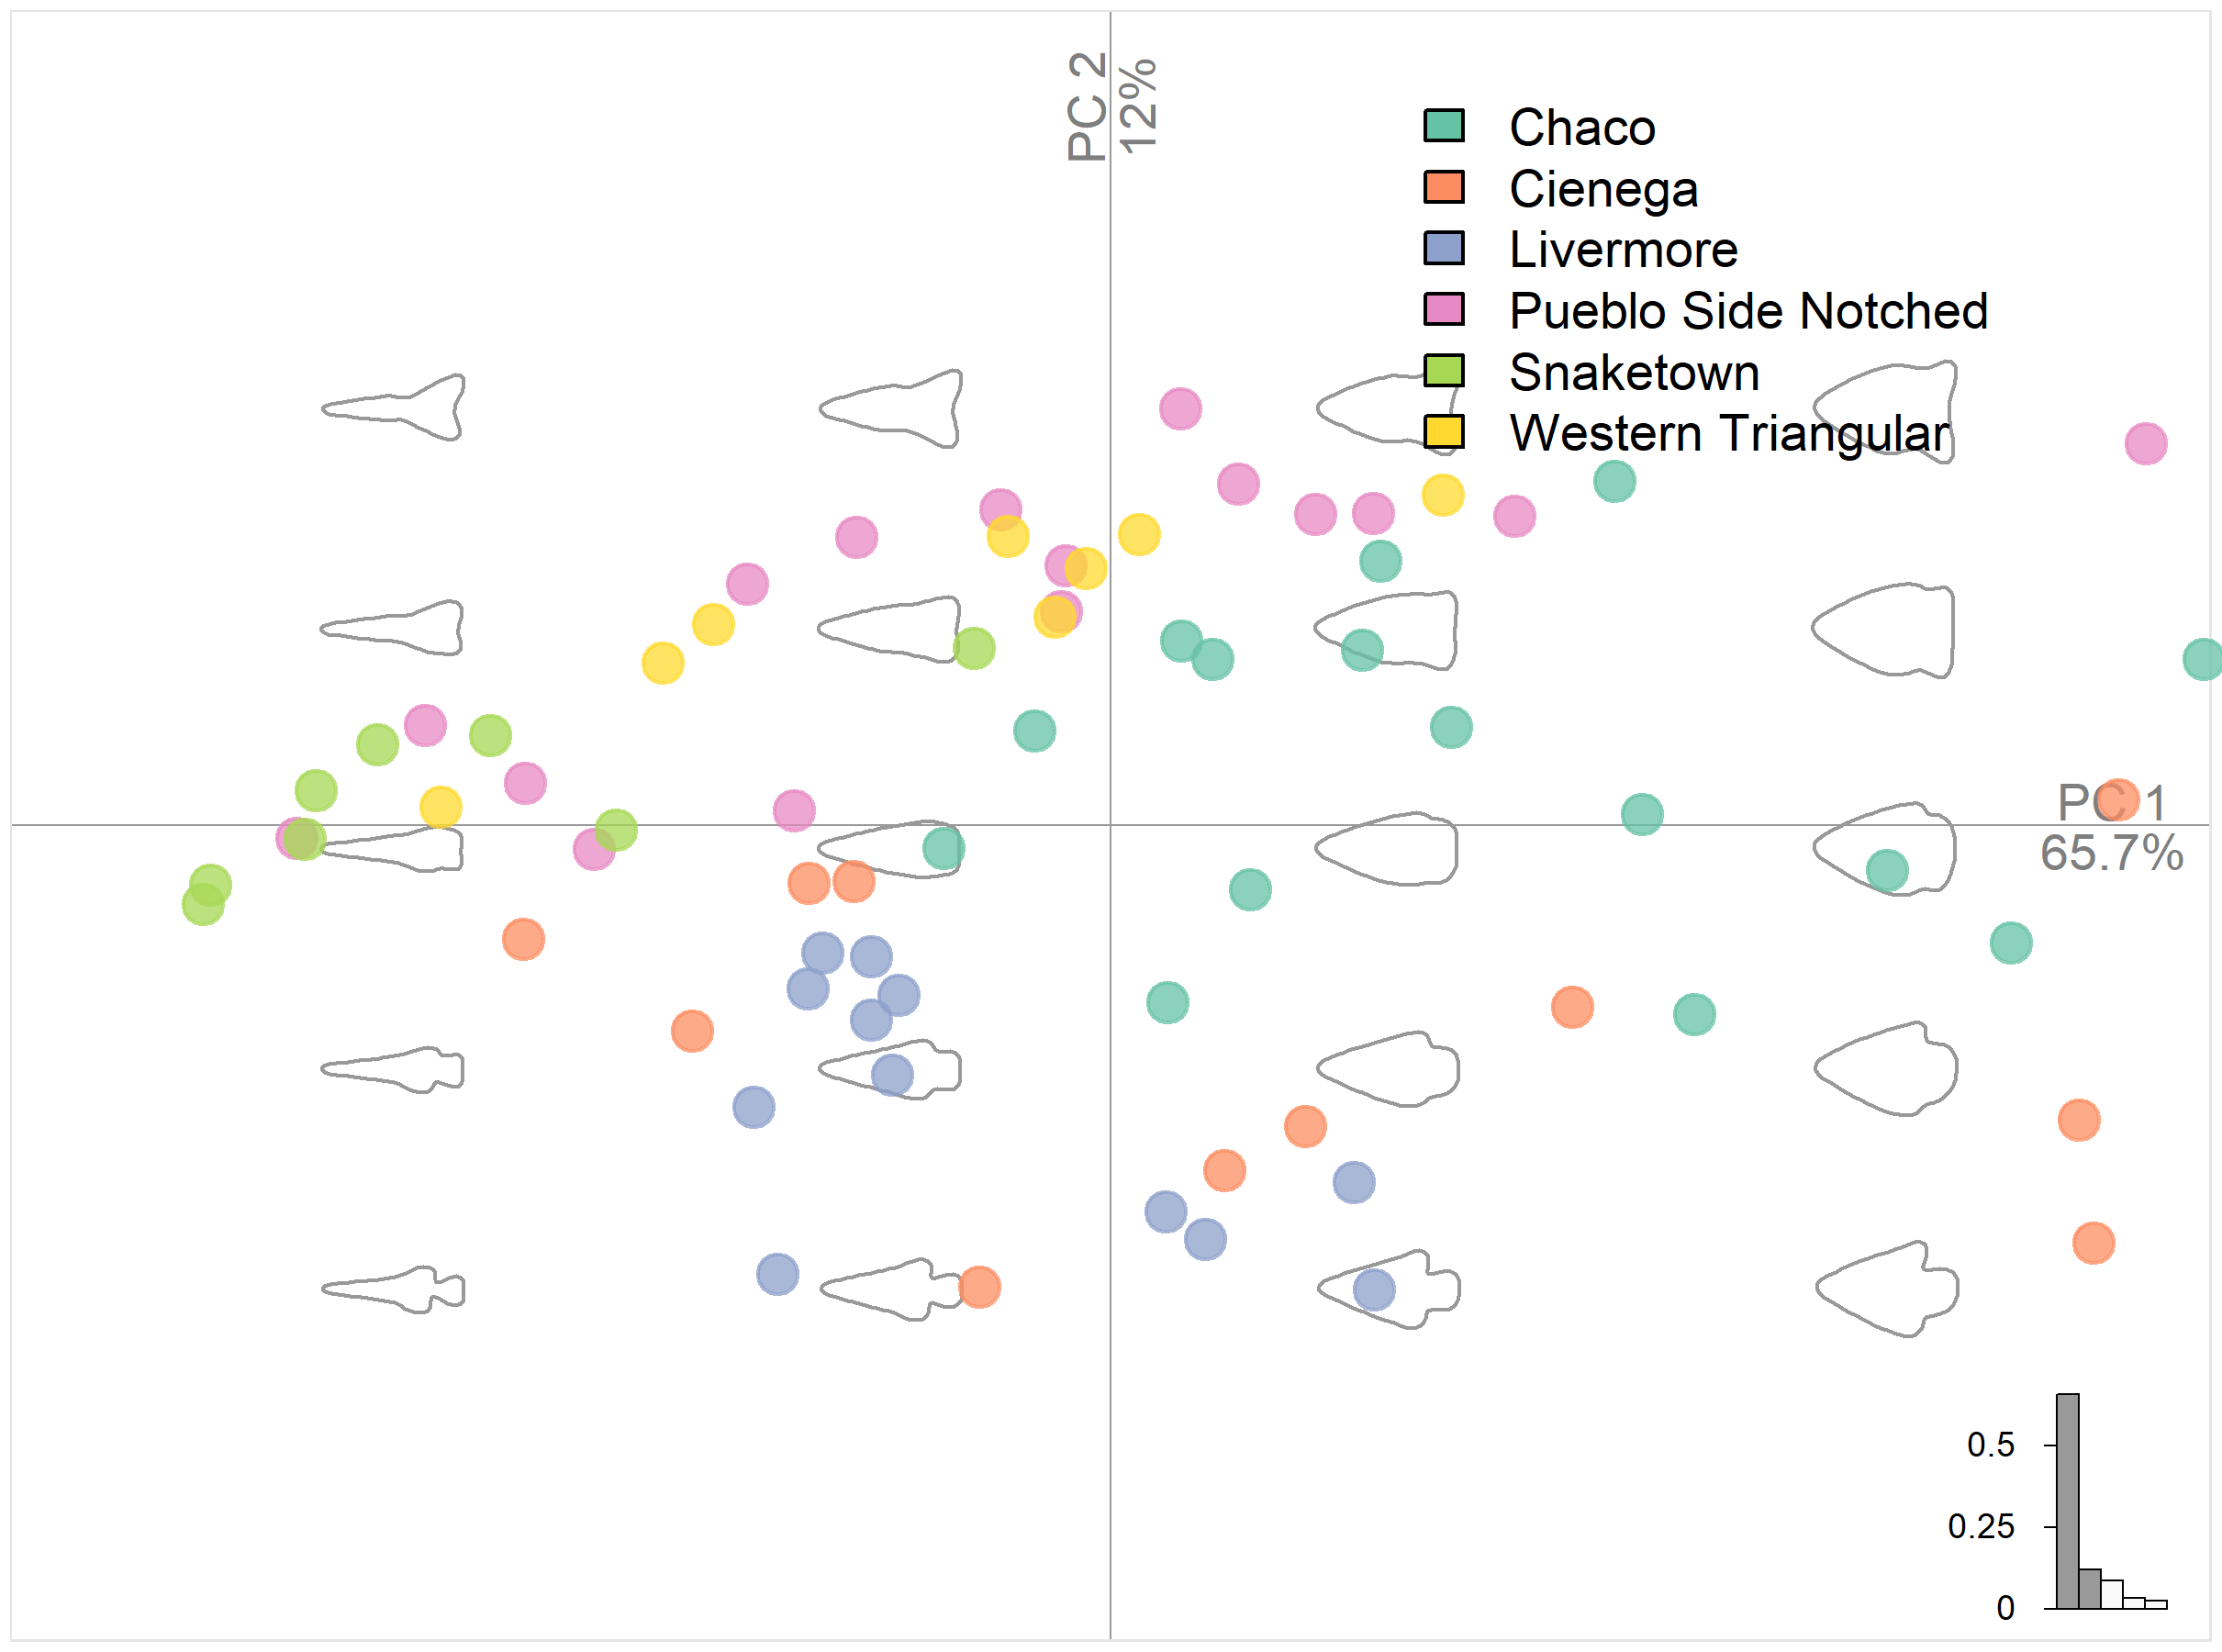
\includegraphics[width=1\linewidth]{figures/JusticeEFAPCA} \caption{Principal components plot showing projectile points from Justice (2002) and the morphospace based on an elliptical Fourier analysis. The points are labeled by the cluster assigned by Justice.}\label{fig:JusticeEFAPCA}
\end{figure}

The first objective for the analysis of the Justice points is to
determine how well the different point types can be discriminated.
Meaning, how well can GM methods classify these points into their
original categories. The LDA results were far from the target goal of
0.85 for most projectile point types, and only one type (Pueblo Alto
Side Notched) met the target (see EFA results in Table 2). The results
were better when the projectile point types were grouped into clusters,
as shown in Table 3; however, none of the clusters met the target of
0.85. Even more disconcerting were the results shown in Table 4, as only
the corner-notched points were discriminated with an accuracy greater
than the target.

The differences in classification accuracy between corner-notched,
side-notched, and triangular points can perhaps best be explained by
examining the mean shapes of each point. Figure 11 shows the mean shapes
for the selected projectile point types. These are the mathematically
average shapes when all of the projectile points in the type are
combined. This has a tendency to average out the notches for the
side-notched points, as the placement of these notches vary in height.
Pueblo Alto Side Notched points appear to be an exception to the
side-notched problem, as they have the highest classification accuracy.
Corner notched and stemmed points must, by definition, always have their
notches or stems in the same location, even though the shape of the
notches and stems still varies. This explains why it is easier to
discriminate them from other point types. As for the side-notched and
triangular points, sometimes the notches are subtle and the notches are
only a small part of the whole form, which is clearly not a strong
enough element to separate triangular and side-notched points
consistently.

\begin{figure}
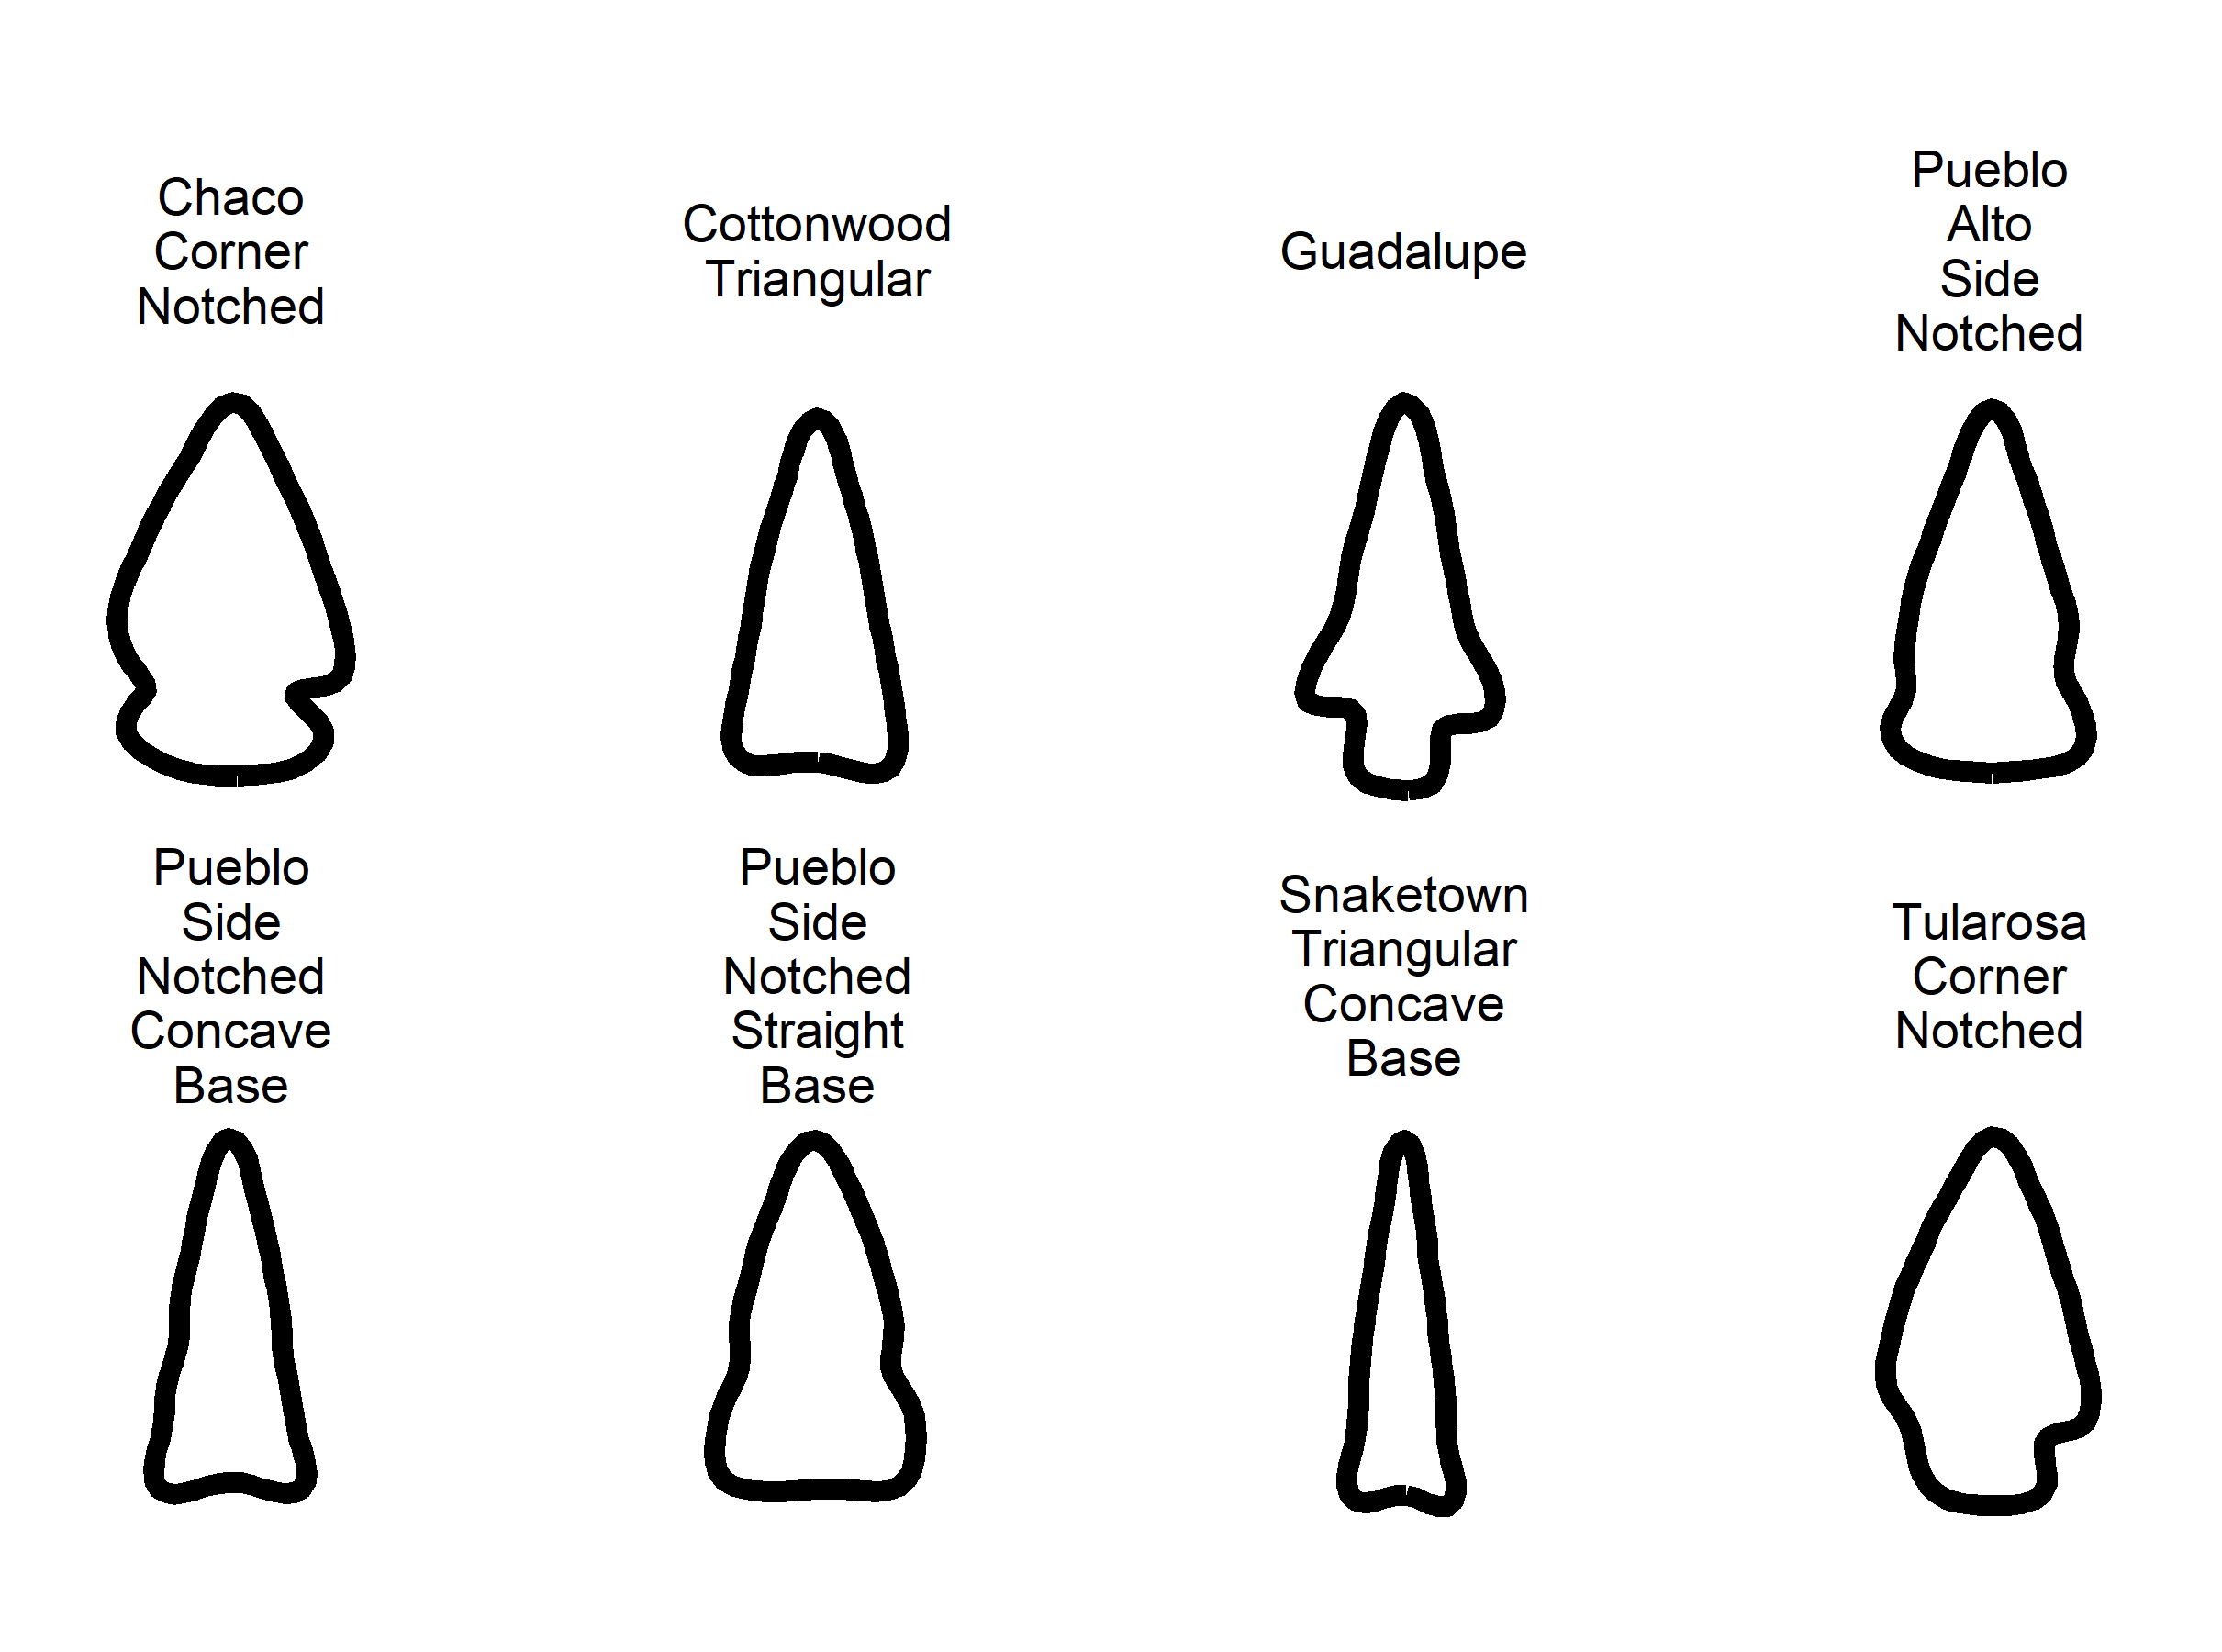
\includegraphics[width=1\linewidth]{figures/meanShapesEFA} \caption{Mean shapes by projectile point type using elliptical Fourier analysis.}\label{fig:meanShapes}
\end{figure}

\hypertarget{semilandmarks}{%
\subsection{Semilandmarks}\label{semilandmarks}}

Analyzing projectile points using semilandmarks is comparable to the EFA
analysis. The major analytical choice is how many landmarks to use. Each
projectile point is represented by a varied number of coordinates that
represent its outline. The number of points must be standardized so that
each projectile point has an identical number of coordinates, which is
done using the Momocs package. The choice of how many points to use does
affect the GM analysis. To solve this problem, I tried different numbers
of semilandmarks varying from 10 to 100. More than 100 points appears to
no longer have a substantial effect on the results. Each projectile
point was sampled multiple times and then all of the points were
classified using LDA according to the same procedures used for the EFA
analysis. The results of this test ranged from 65\% accuracy (10 points)
to 73\% accuracy (30 points--the number used for the final analysis)
with somewhat higher numbers of points consistently measuring in at 64\%
accuracy.

The morphospace (see figure 12) based on the PCA analysis has similar
dimensions of variation as the EFA analysis. The major improvement in
accuracy (the 'semiLdk column of Tables 2-4) is perhaps due to the
better alignment generated by the GPA procedure, but that is only
speculation.

\begin{figure}
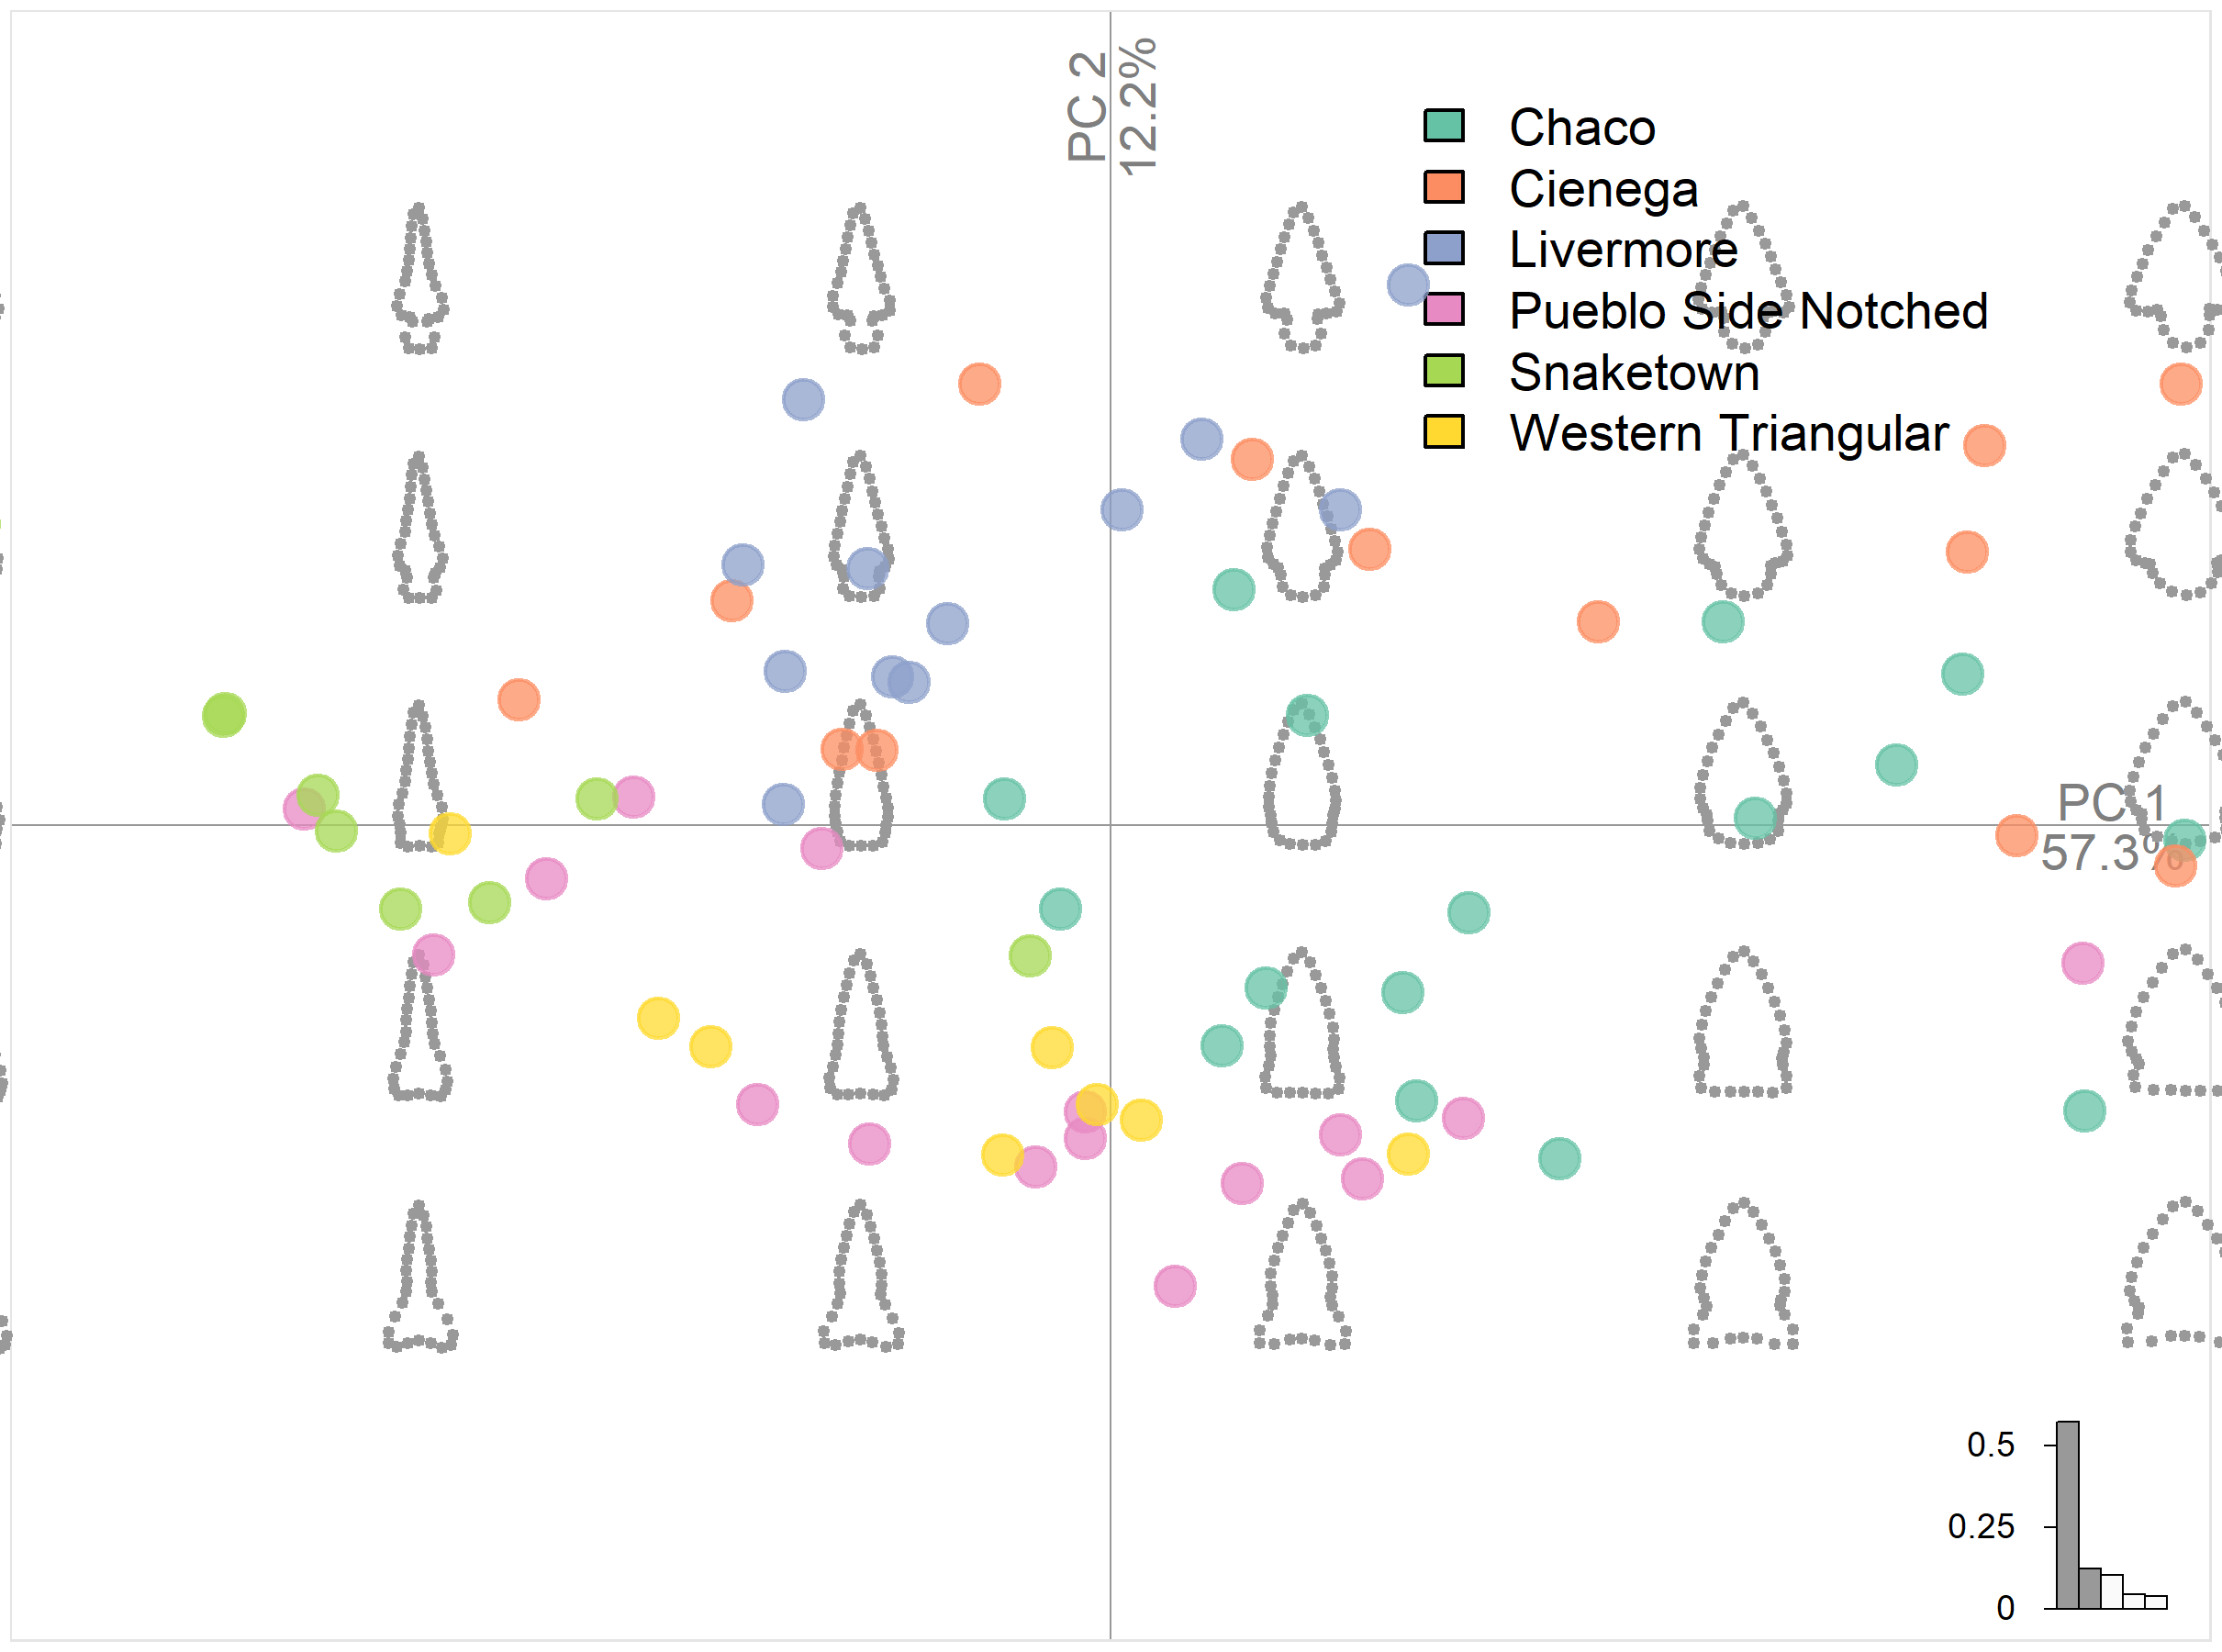
\includegraphics[width=1\linewidth]{figures/JusticeSLDKPCA} \caption{Principal Components Plots showing projectile points from Justice (2002) and the morphospace based on a semilandmark generalized procrustes alignment. The points are labeled by the cluster assigned by Justice.}\label{fig:JusticeSLDKPCA}
\end{figure}

Regardless of the reason, a jump from 64\% classification to 72\% is a
substantial improvement. It does not reach the target of greater than
85\% classification accuracy, but it is a step in the right direction.
The mean shapes are nearly identical to the EFA analysis, which
indicates that this method suffers from the same problems with
side-notched and triangular points, but it does a somewhat better job
differentiating corner-notched and side-notched points. Curiously, it
does a worse job differentiating triangular points. It seems the
side-notches are still a problem.

\hypertarget{landmarks}{%
\subsection{Landmarks}\label{landmarks}}

Neither the semilandmarks nor EFA adequately distinguished between point
types or between point shapes. Identifying notches was particularly
troublesome. A solution to this problem was to use landmarks and
explicitly identify the notches or lack of notches. No comparison was
made between projectile point shapes using landmark analysis, as initial
experiments determined that it was best to use different landmark
procedures for the different shapes. Perhaps machine learning may solve
this problem (see
\protect\hyperlink{ref-Castillo_Flores2019-cs}{Castillo Flores et al.
2019}; \protect\hyperlink{ref-MacLeod2018-aj}{MacLeod 2018};
\protect\hyperlink{ref-Nash2016-mc}{Nash and Prewitt 2016}). Triangular
points require a different approach than side-notched points, and even
side-notched and corner-notched/stemmed points require different
procedures.

The LDA results for the first landmark configuration (Ldk in Tables 2-4)
are much better than EFA and better than the semilandmark analysis, but
still not as accurate as desired. The biggest underperformer by far was
Pueblo Side Notched Straight Base at 0.43. All of the previous analyses
struggled to capture basal shape distinctions, but this analysis
struggled more so. What is particularly notable is that Cottonwood
Triangular points were classified perfectly whereas they were previously
the worst performing type. As Table 3 shows, the cluster assignments
performed well. If the problems sorting Cienega from Snaketown can be
sorted out, then the results would be excellent.

The final analysis used the second landmark configuration--the
projectile point corners. These results proved superior to the first
landmark configuration and are almost 20\% points higher in accuracy
than the EFA results on average. The lowest type for accuracy was again
Pueblo Side Notched Straight Base, but it improved from the first
landmark configuration to 0.71 from 0.43. The accuracy results were more
consistent and accurate. With some enhancement, this configuration could
likely achieve better results.

Not only did landmark analysis provide superior accuracy, but it will
also make it easier to use larger sample sizes. Presumably, notching
style is an important attribute that should be captured in the analysis.
If EFA or the semilandmark analysis as conducted here fails to
sufficiently emphasize the notches, then these methods are insufficient
for my purposes. While landmark analysis is more time-consuming, the use
of the second configuration does reduce the burden of landmarking.

\hypertarget{tonto-basin-points}{%
\section{Tonto Basin Points}\label{tonto-basin-points}}

The initial intent was to classify the Tonto Basin points using the
analysis of the Justice points; however, the limited sample size limits
the validity of the exercise. The analysis was not futile though, as the
second landmark configuration using the corners of the projectile points
proved the most effective. I therefore used the same landmark
configuration to analyze the points from Tonto Basin. The results of the
GPA and PCA analysis were used in a hierarchical cluster analysis using
Ward's method (see \protect\hyperlink{ref-Murtagh2014-mb}{Murtagh and
Legendre 2014}). Figure 13 is a network graph showing the results.
Several sites in Tonto Basin only had one or two types of projectile
points (low sample sizes were again problematic), but some of the
larger, well-excavated sites shared all or most of the projectile point
types. It is beyond the purpose of this study to explore the patterns in
this data, but the methods clearly provide useful data for exploratory
analysis.

\begin{figure}
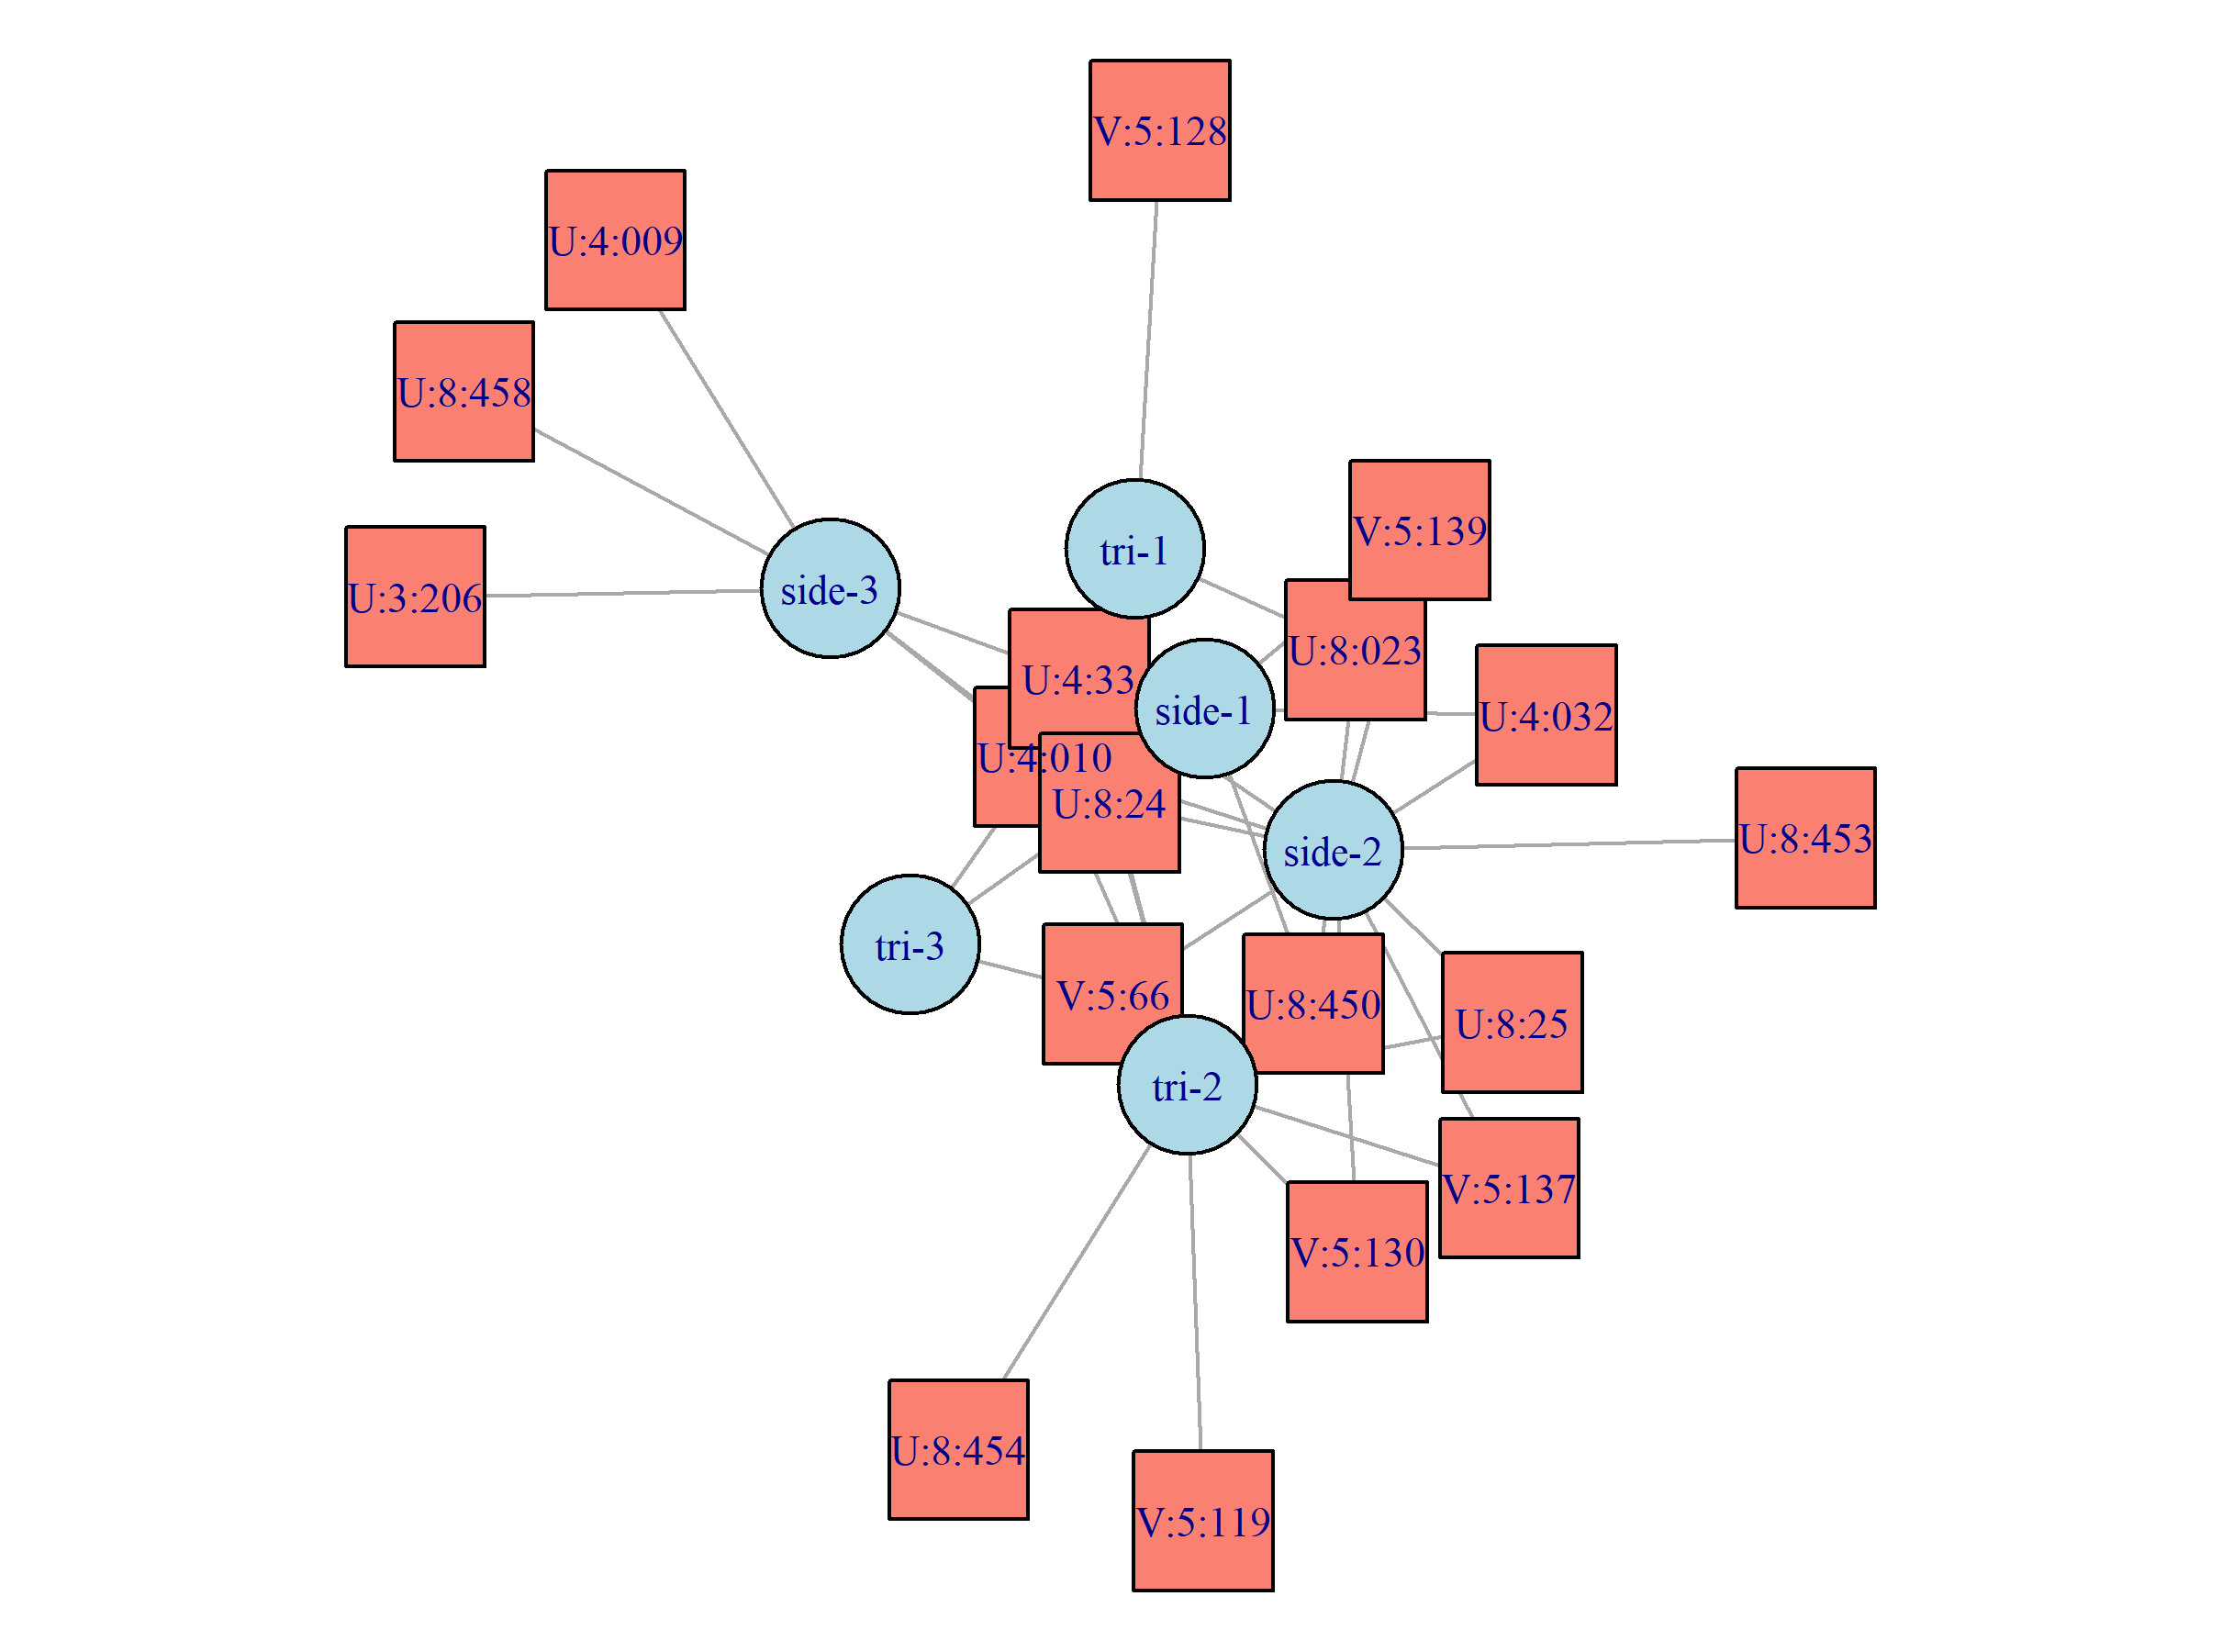
\includegraphics[width=1\linewidth]{figures/TontoClusterNetwork} \caption{Bipartite network graph displaying assigned projectile point clusters for side-notched and triangular points in Tonto Basin and Tonto Basin sites.}\label{fig:TontoClusterNetwork}
\end{figure}

The final question I wished to address in this study was whether it was
necessary to use a typology in a GM analysis of projectile points. There
are many ways to answer this question, but in short, the answer is no.
That does not mean typologies are not useful, but they can mask
important variation. The following is one way to approach analyzing
projectile points without using a typology.

Because the results of the GM analyses can be projected into
multidimensional space, the distance between these values is meaningful
and can be directly compared. One way to flatten multidimensional space
is to calculate the Euclidean distance between each point and display
the results as a network graph, as in figures 14 and 15. This way each
point can be compared directly without grouping the points into types.
The results are messier, but subtle variation in morphology is easier to
visualize this way. The closer the points are to each other, the more
similar they are in shape, keeping in mind that only the corners of the
projectile points (from the notches down for the side-notched points)
were used in this analysis. Many of the points clustered closely
together, indicating a common shape across the sites. The side-notched
points have a particularly large cluster of typical Hohokam side-notched
points. Yet there are also a large number of points that do not closely
match the points, which indicates that there is also a lot of variation.
This variation may represent idiosyncracies, exchange, migration, novice
knappers, or a different intention for the point. Regardless of the
purpose, the GM analysis better captures the ``otherness'' of a point
than classifying a point as other/unknown or worse, forcing it into a
category it does not belong in.

\begin{figure}
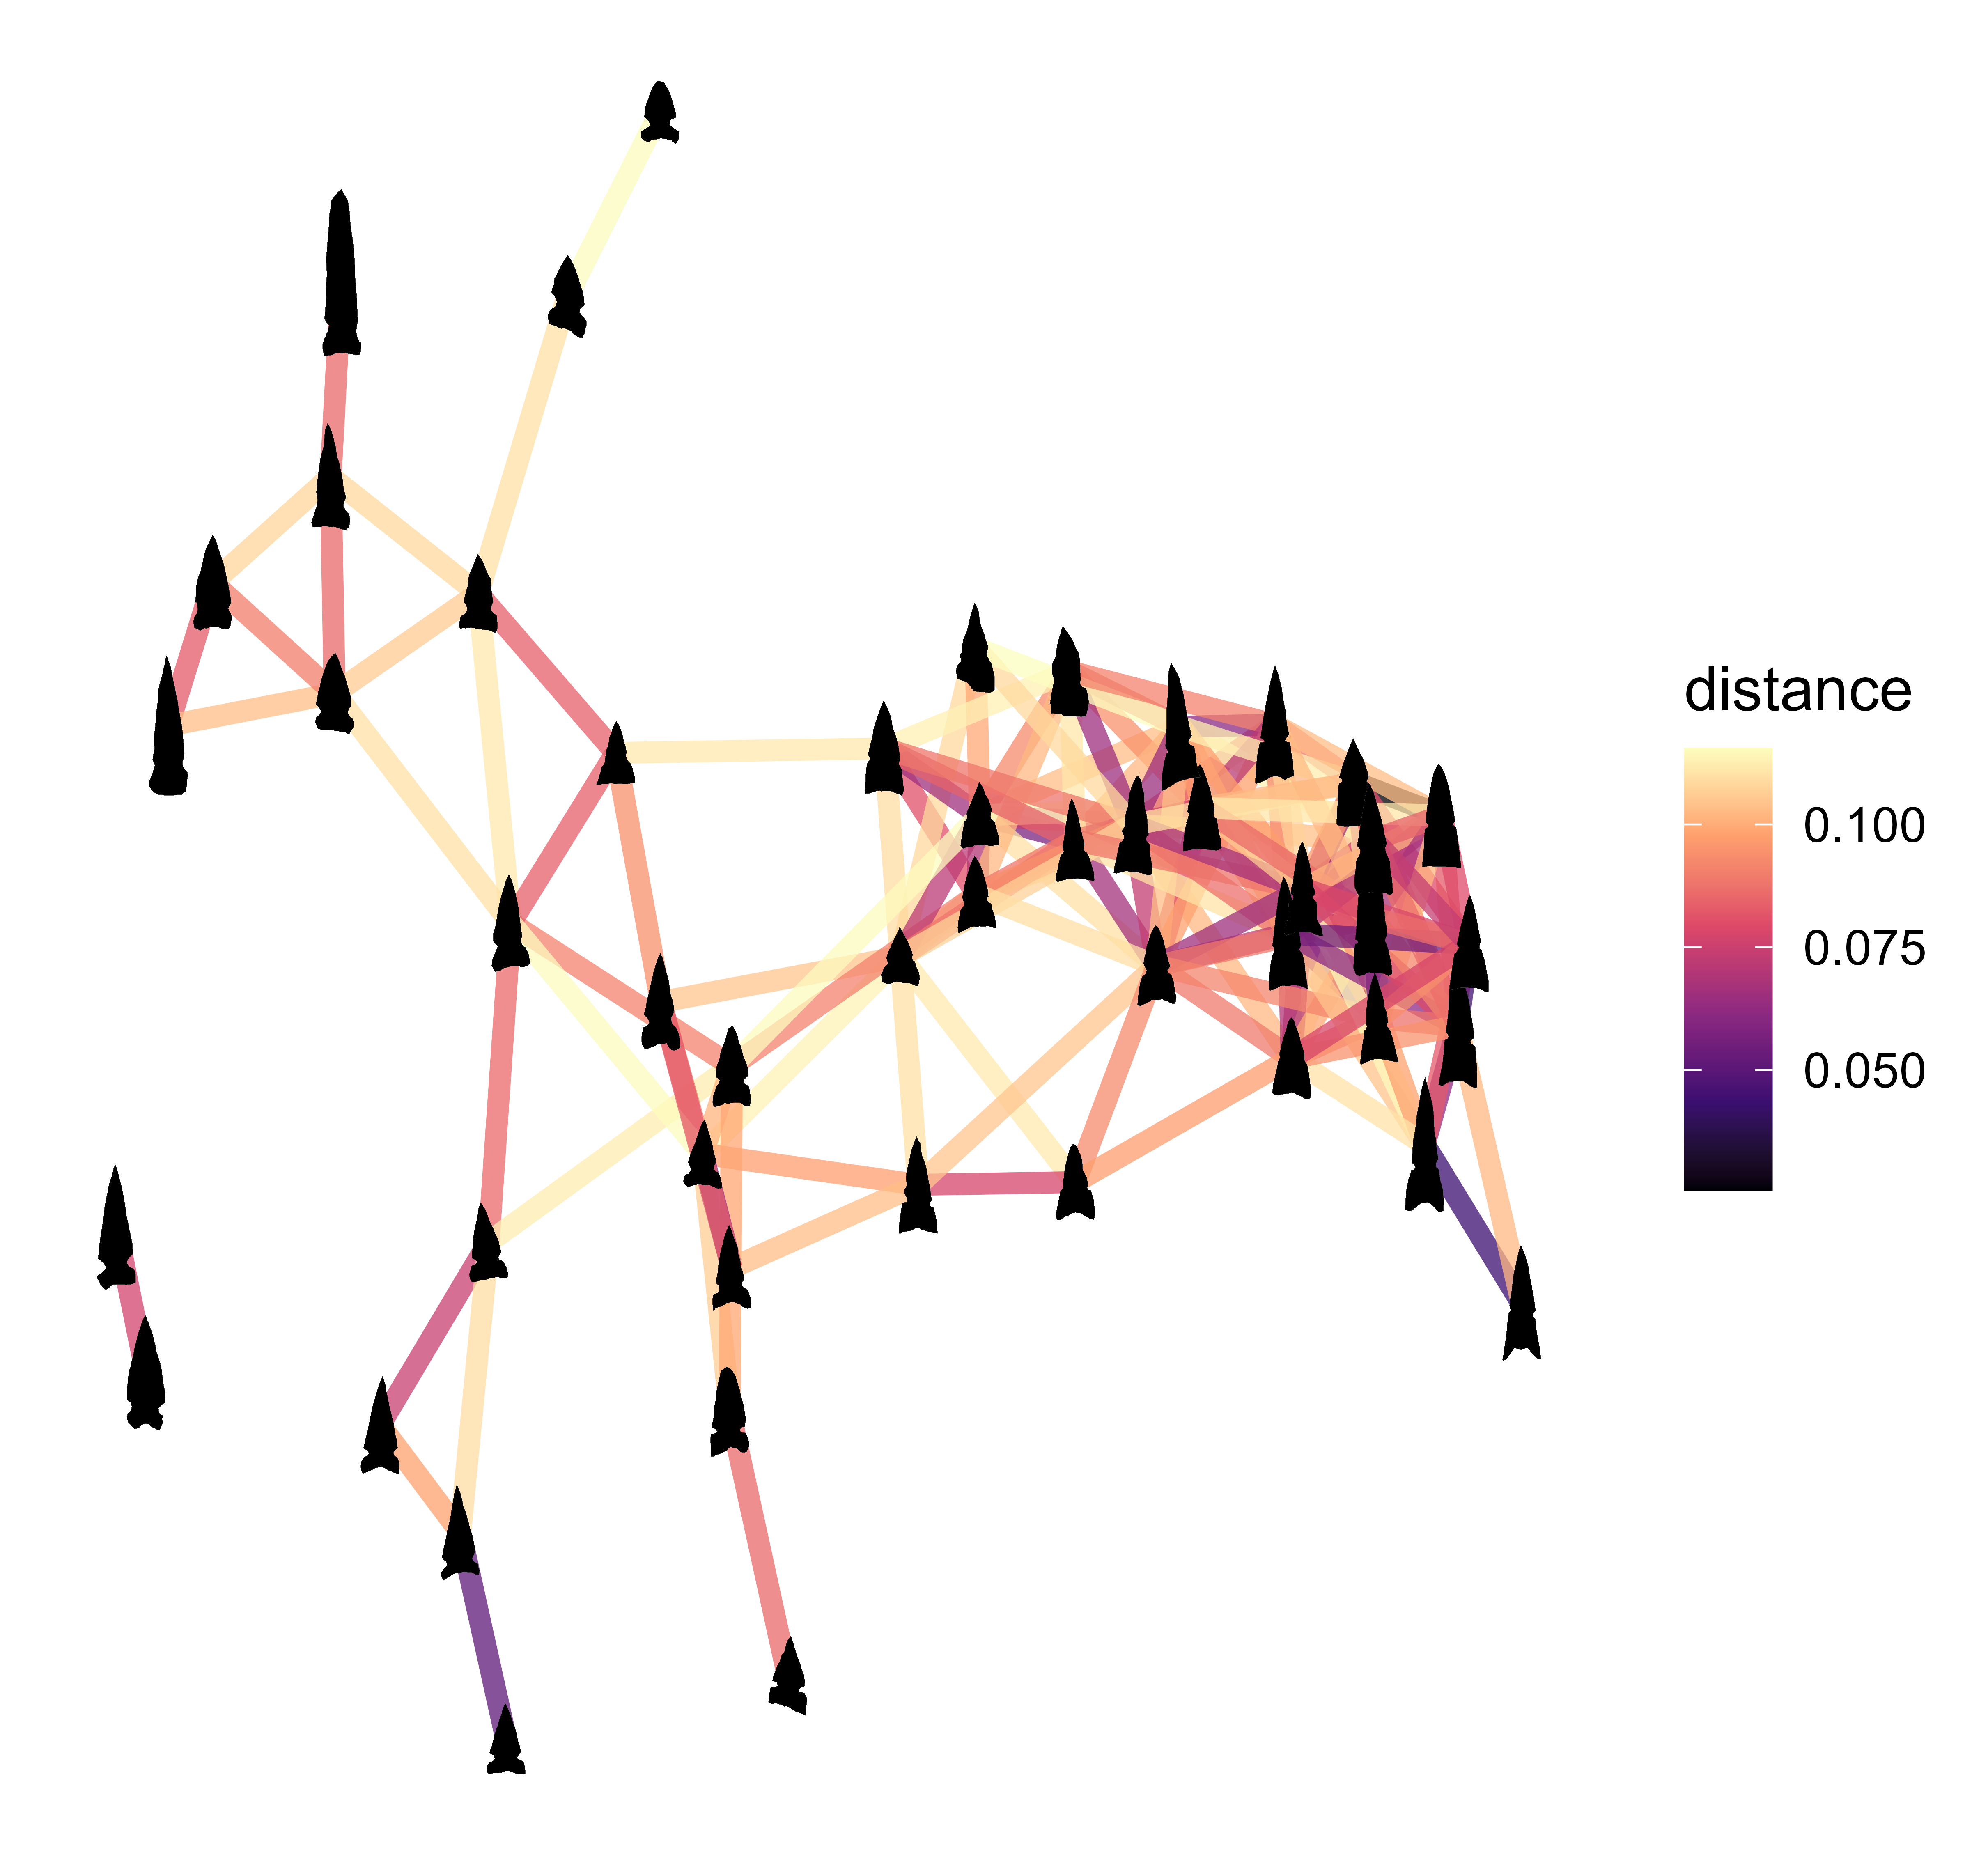
\includegraphics[width=1\linewidth]{figures/TontoSideDistanceNetwork} \caption{Network graph displaying side-notched points from Tonto Basin as nodes with ties showing the morphometric distance between points. Darker colors represent stronger ties. Note that only the strongest 10\% of ties are shown.}\label{fig:TontoSideDistanceNetwork}
\end{figure}

\begin{figure}
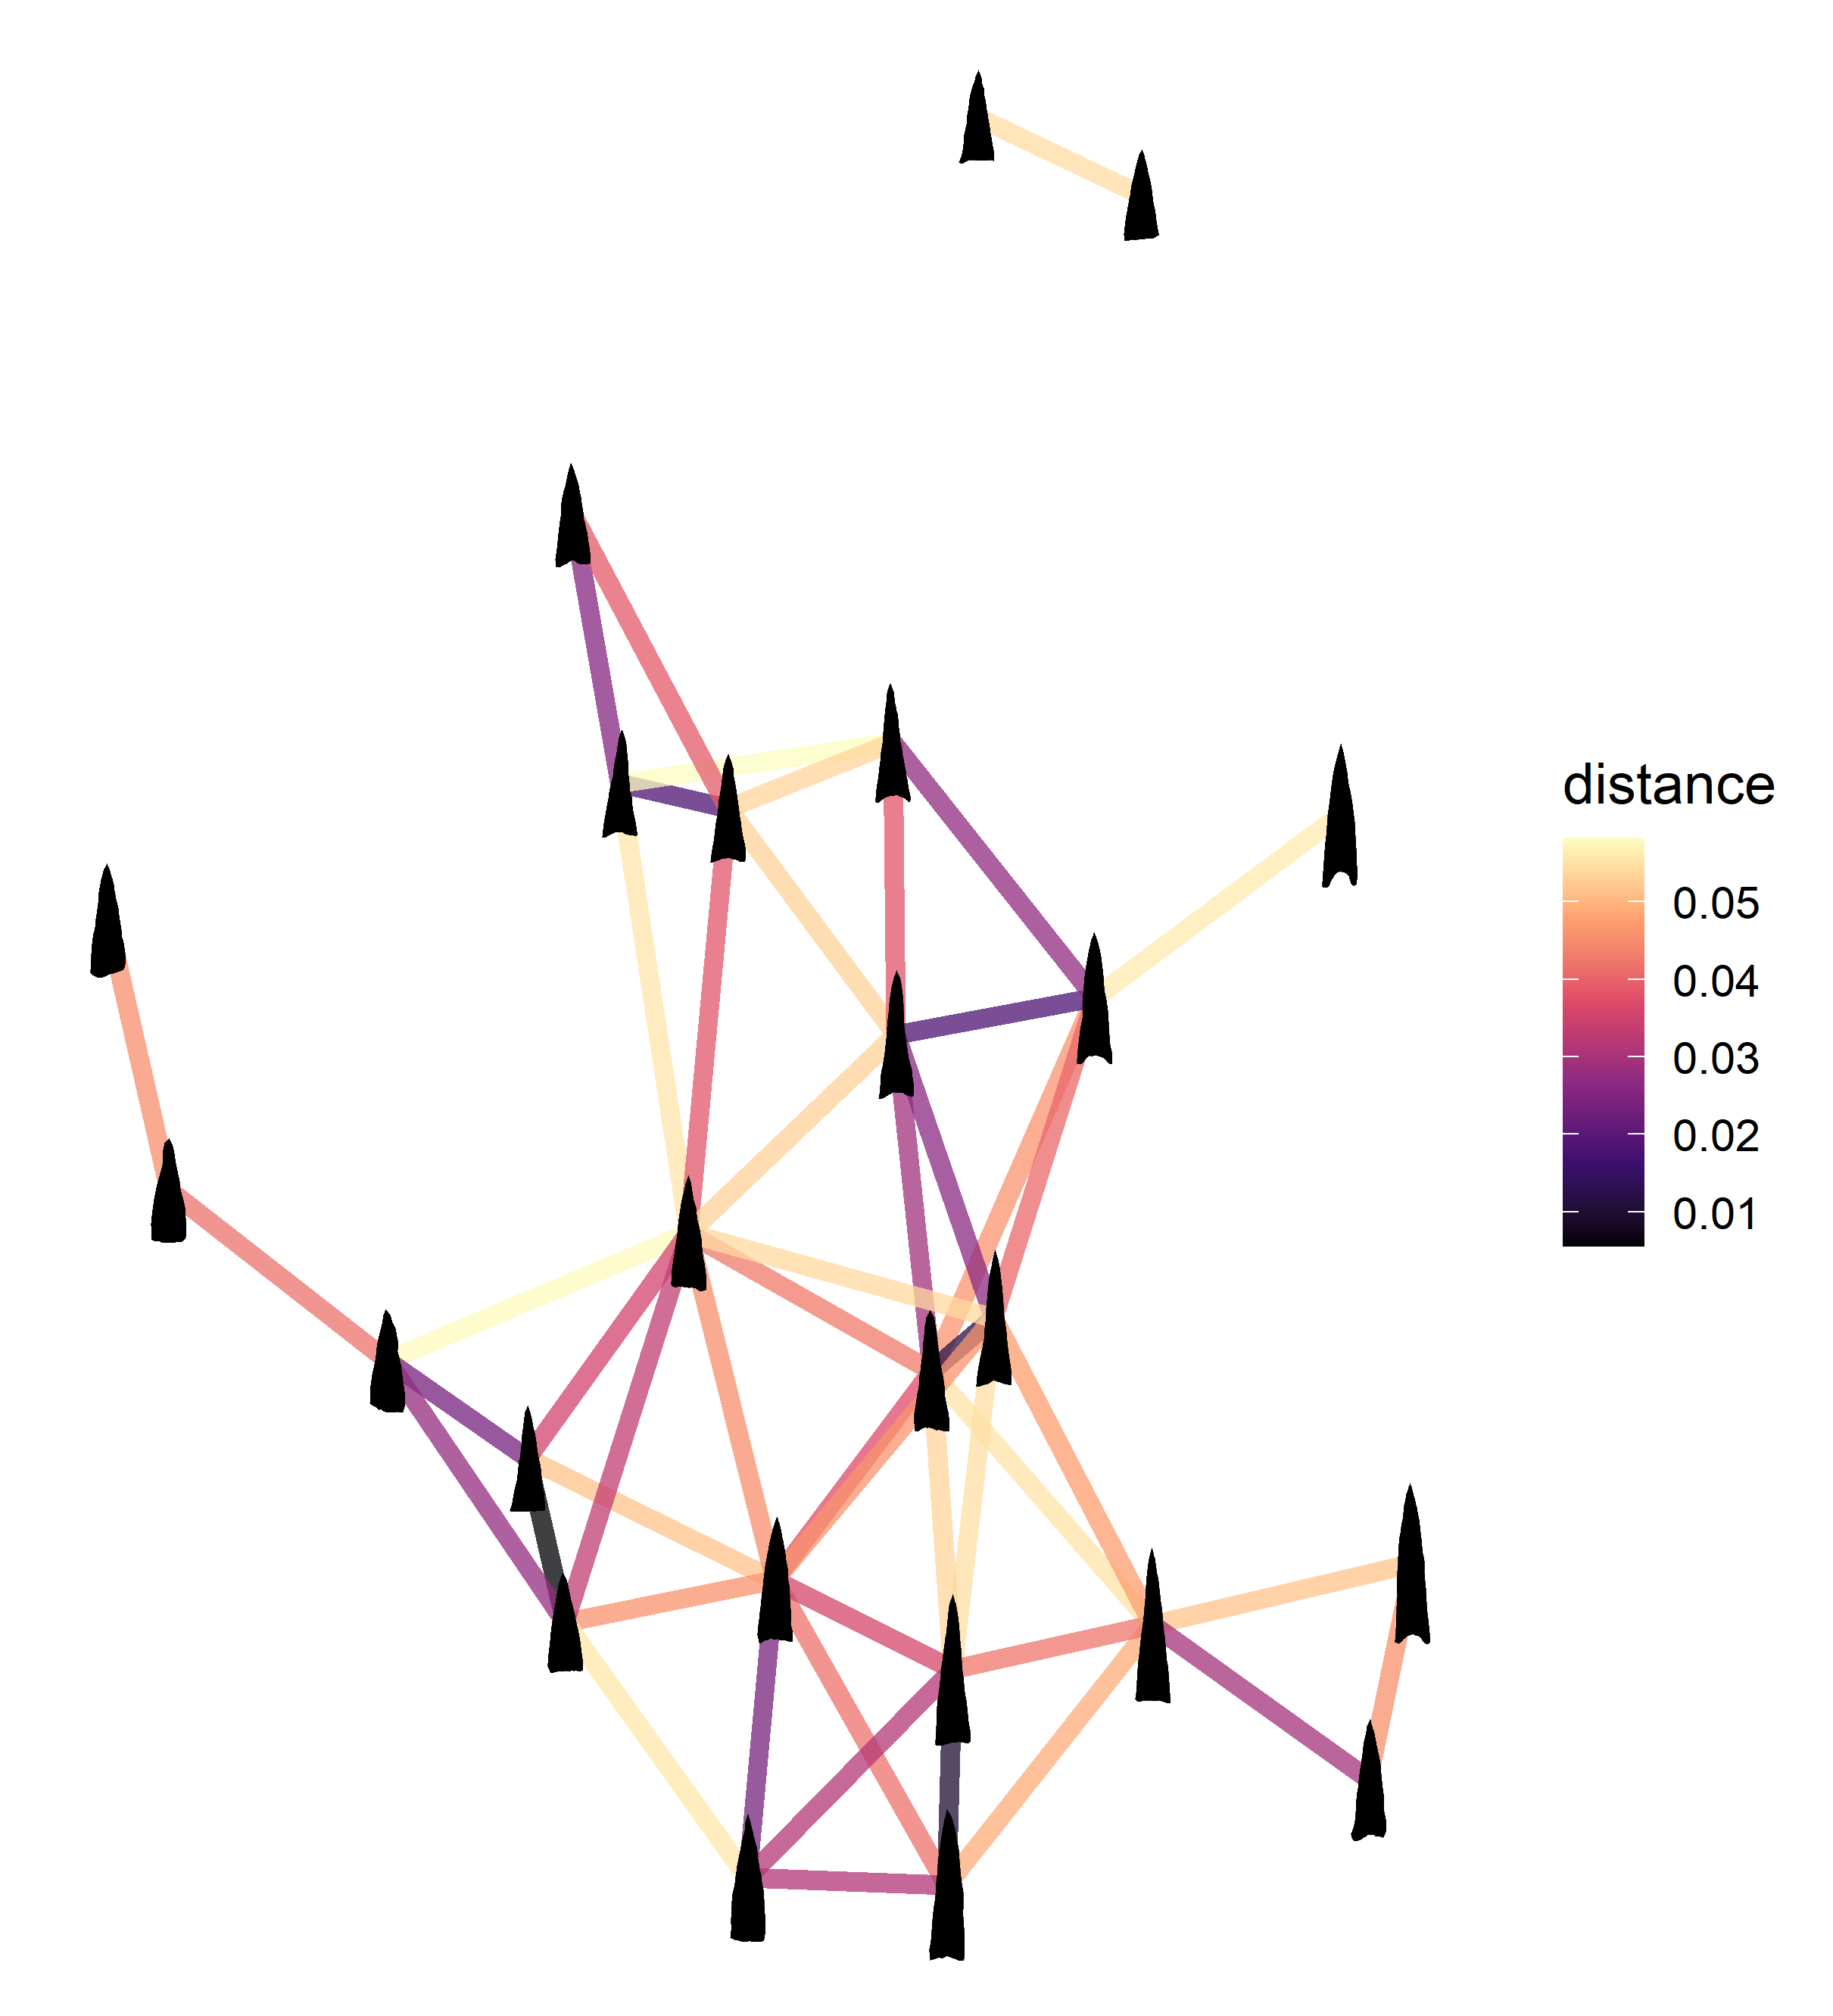
\includegraphics[width=1\linewidth]{figures/TontoTriangularDistanceNetwork} \caption{Network graph displaying triangular points from Tonto Basin as nodes with ties showing the morphometric distance between points. Darker colors represent stronger ties. Note that only the strongest 10\% of ties are shown.}\label{fig:TontoTriangularDistanceNetwork}
\end{figure}

The clustering analysis provided several different projectile point
types and provided an overview of what sites shared similar projectile
points. This type of analysis can be combined with architectural or
other data to look for correlations or patterns that provide insights
into the behavior of the people who made and used these points. Yet the
analyst must take care to ensure the clustering groups are appropriately
sized and the results make sense. One way to view the data more closely
is to look at a distance network graph to view the variation in
morphometric shape. This way typological distinctions will not mask the
variation.

\hypertarget{conclusion}{%
\section{Conclusion}\label{conclusion}}

These analyses provided significant variation in their results, yet they
also demonstrated positive results. While EFA underperformed all of the
other analyses, a different dataset may favor this analysis. Some of the
types performed better for EFA than other types, which suggests that EFA
may be the optimal choice for some datasets. A clear result from this
exploratory analysis is that GM analysis is not a one-size-fits-all
approach. In this case, using the corner of the projectile point--from
the base to the middle of the basal margin or from the middle of the
blade if the point is triangular--proved to be the most useful method.
The main advantage of this method was that it provided the most accurate
reproduction of Justice's original classification of the projectile
points. Another advantage is that broken points are easier to use with
this method. If one half of the point is missing, either the top or the
lateral margin, it does not affect the analysis. This increases the
number of points available for analysis tremendously compared to only
using whole points. The final advantage, though minor, is that the
landmarking analysis is simple and only requires three to five
landmarks.

I mentioned in the introduction how difficult it is to conduct regional
analyses with projectile points in the U.S. Southwest. The main
difficulty is harmonizing existing typologies and then fitting new
projectile points into this typology. While the sample size available
for this study was too small to attempt classifying the Tonto Basin
points according to Justice's typology, it would be possible to do so
with these methods. However, this chapter also demonstrated that it is
possible to type points using common clustering methods which may better
capture the variation in projectile point morphology than previously
used types. Furthermore, it is possible to analyze projectile points
without resorting to types. The distances between projectile point
morphologies can be computed and compared directly. These distances
could even be aggregated and summarized regionally. The main challenge
for the regional analysis is obtaining the projectile point outlines or
landmarks. Once these are obtained, thousands of points can be analyzed
and assigned to clusters relatively quickly.

Compared to a traditional analysis of linear metrics and weights, a GM
analysis can capture much more information and provide more informative
ways to analyze and visualize the data. The visualization capabilities
of GM is one of its greatest strengths, as it allows the analyst to see
the data they are working with, visually validate their results, and
share their findings in visually compelling ways. Additionally, this
analysis is more reproducible and adaptable than traditional lithic
analyses. While the analyst still has a lot of control over a GM
analysis, the results should be less biased than analyses based on
visual type comparisons.

\hypertarget{references}{%
\section*{References}\label{references}}
\addcontentsline{toc}{section}{References}

\hypertarget{refs}{}
\begin{CSLReferences}{1}{0}
\leavevmode\vadjust pre{\hypertarget{ref-Archer2018-zi}{}}%
Archer, W, C M Pop, Z Rezek, S Schlager, S C Lin, M Weiss, T Dogandžić,
D Desta, and S P McPherron. 2018. {``{A geometric morphometric
relationship predicts stone flake shape and size variability}.''}
\emph{Archaeological and Anthropological Sciences} 10 (8): 1991--2003.

\leavevmode\vadjust pre{\hypertarget{ref-Bernardini2005-ue}{}}%
Bernardini, Wesley. 2005. \emph{{Hopi Oral Tradition and the Archaeology
of Identity}}. Tucson: University of Arizona Press.

\leavevmode\vadjust pre{\hypertarget{ref-Bischoff2020-zn}{}}%
Bischoff, Robert J, and James R Allison. 2020. {``{Rosegate Projectile
Points in the Fremont Region}.''} \emph{Utah Archaeology} 33 (1): 7--48.
\url{https://doi.org/10.31235/osf.io/dwrba}.

\leavevmode\vadjust pre{\hypertarget{ref-Bonhomme2014-gt}{}}%
Bonhomme, Vincent, Sandrine Picq, Cédric Gaucherel, and Julien Claude.
2014. {``{Momocs: Outline Analysis Using R}.''} \emph{Journal of
Statistical Software, Articles} 56 (13): 1--24.
\url{https://doi.org/10.18637/jss.v056.i13}.

\leavevmode\vadjust pre{\hypertarget{ref-Buchanan2015-dx}{}}%
Buchanan, Briggs, Metin I Eren, Matthew T Boulanger, and Michael J
O'Brien. 2015. {``{Size, Shape, Scars, and Spatial Patterning: a
Quantitative Assessment of Late Pleistocene (Clovis) Point
Resharpening}.''} \emph{Journal of Archaeological Science: Reports} 3
(September): 11--21. \url{https://doi.org/10.1016/j.jasrep.2015.05.011}.

\leavevmode\vadjust pre{\hypertarget{ref-Buchanan2019-vn}{}}%
Buchanan, Briggs, Marcus J Hamilton, James C Hartley, and Steven L Kuhn.
2019. {``{Investigating the Scale of Prehistoric Social Networks Using
Culture, Language, and Point Types in Western North America}.''}
\emph{Archaeological and Anthropological Sciences} 11 (January):
199--207. \url{https://doi.org/10.1007/s12520-017-0537-y}.

\leavevmode\vadjust pre{\hypertarget{ref-Caple2017-mk}{}}%
Caple, Jodi, John Byrd, and Carl N Stephan. 2017. {``Elliptical Fourier
Analysis: Fundamentals, Applications, and Value for Forensic
Anthropology.''} \emph{International Journal of Legal Medicine} 131 (6):
1675--90. \url{https://doi.org/10.1007/s00414-017-1555-0}.

\leavevmode\vadjust pre{\hypertarget{ref-Cardillo2010-ys}{}}%
Cardillo, Marcelo. 2010. {``{Some Applications of Geometric
Morphometrics to Archaeology}.''} In \emph{{Morphometrics for
Nonmorphometricians}}, edited by Ashraf M T Elewa, 325--41. Berlin:
Springer. \url{https://doi.org/10.1007/978-3-540-95853-6}.

\leavevmode\vadjust pre{\hypertarget{ref-Castillo_Flores2019-cs}{}}%
Castillo Flores, Fernando, Francisco García Ugalde, Díaz Luis Punzo,
Jesús Zarco Navarro, Gastelum-strozzi, Alfonso, María Del pilar Angeles,
and Mariko Nakano Miyatake. 2019. {``{Computer Algorithm for
Archaeological Projectile Points Automatic Classification}.''}
\emph{Journal on Computing and Cultural Heritage (JOCCH)} 12 (3): 19.
\url{https://doi.org/10.1145/3300972}.

\leavevmode\vadjust pre{\hypertarget{ref-Charlin2018-yg}{}}%
Charlin, Judith, and Rolando González-José. 2018. {``{Testing an
Ethnographic Analogy Through Geometric Morphometrics: A Comparison
Between Ethnographic Arrows and Archaeological Projectile Points from
Late Holocene Fuego-Patagonia}.''} \emph{Journal of Anthropological
Archaeology} 51 (September): 159--72.
\url{https://doi.org/10.1016/j.jaa.2018.06.008}.

\leavevmode\vadjust pre{\hypertarget{ref-Clark2019-bz}{}}%
Clark, Jeffery J, Jennifer A Birch, Michelle Hegmon, Barbara J Mills,
Donna M Glowacki, Scott G Ortman, Jeffrey S Dean, et al. 2019.
{``{Resolving the Migrant Paradox: Two Pathways to Coalescence in the
Late Precontact U.S. Southwest}.''} \emph{Journal of Anthropological
Archaeology} 53 (March): 262--87.
\url{https://doi.org/10.1016/j.jaa.2018.09.004}.

\leavevmode\vadjust pre{\hypertarget{ref-Colton1956-zy}{}}%
Colton, Harold S. 1956. \emph{{Pottery Types of the Southwest}}. Museum
of Northern Arizona Ceramic Series No. 3c. Flagstaff, Arizona: Museum of
Northern Arizona.

\leavevmode\vadjust pre{\hypertarget{ref-De_Groote2011-mh}{}}%
De Groote, Isabelle. 2011. {``{Femoral Curvature in Neanderthals and
Modern Humans: A {3D} Geometric Morphometric Analysis}.''} \emph{Journal
of Human Evolution} 60 (5): 540--48.
\url{https://doi.org/10.1016/j.jhevol.2010.09.009}.

\leavevmode\vadjust pre{\hypertarget{ref-Duff1996-au}{}}%
Duff, Andrew I. 1996. {``{Ceramic {micro-Seriation}: Types or
Attributes?}''} \emph{American Antiquity} 61 (1): 89.
\url{https://doi.org/10.2307/282304}.

\leavevmode\vadjust pre{\hypertarget{ref-Fisher2018-jq}{}}%
Fisher, Philip Robert. 2018. {``{Understanding Culture History using
Topographic Morphometrics of Lithic Projectile Points: Paleoindian Case
Studies from the Great Plains and Northern Alaska}.''} PhD thesis, PhD
Thesis, Department of Anthropology, Washington State University,
Pullman.

\leavevmode\vadjust pre{\hypertarget{ref-Fox2015-ox}{}}%
Fox, Amy N. 2015. {``{A Study of Late Woodland Projectile Point Typology
in New York using Elliptical Fourier Outline Analysis}.''} \emph{Journal
of Archaeological Science: Reports} 4 (December): 501--9.
\url{https://doi.org/10.1016/j.jasrep.2015.10.022}.

\leavevmode\vadjust pre{\hypertarget{ref-Gingerich2014-cb}{}}%
Gingerich, Joseph A M, Sabrina B Sholts, Sebastian K T S Wärmländer, and
Dennis Stanford. 2014. {``{Fluted point manufacture in eastern North
America: an assessment of form and technology using traditional metrics
and 3D digital morphometrics}.''} \emph{World Archaeology} 46 (1):
101--22. \url{https://doi.org/10.1080/00438243.2014.892437}.

\leavevmode\vadjust pre{\hypertarget{ref-gladwin1930a}{}}%
Gladwin, Winifred, and Harold S. Gladwin. 1930. {``Some Southwestern
Pottery Types: Series II.''} \emph{Medallion Papers}, no. 7.

\leavevmode\vadjust pre{\hypertarget{ref-Gower1975-uv}{}}%
Gower, J C. 1975. {``{Generalized Procrustes Analysis}.''}
\emph{Psychometrika} 40 (1): 33--51.

\leavevmode\vadjust pre{\hypertarget{ref-Gunz2009-yb}{}}%
Gunz, Philipp, Philipp Mitteroecker, Simon Neubauer, Gerhard W Weber,
and Fred L Bookstein. 2009. {``{Principles for the virtual
reconstruction of hominin crania}.''} \emph{Journal of Human Evolution}
57 (1): 48--62. \url{https://doi.org/10.1016/j.jhevol.2009.04.004}.

\leavevmode\vadjust pre{\hypertarget{ref-Hargrave1932-ng}{}}%
Hargrave, L Lyndon. 1932. \emph{{Guide to Forty Pottery Types from the
Hopi Country and the San Francisco Mountains, Arizona}}. Vol. Museum of
Northern Arizona Bulletin, No. 1. Flagstaff.

\leavevmode\vadjust pre{\hypertarget{ref-Hegmon2016-xw}{}}%
Hegmon, Michelle, Jacob Freeman, Keith W Kintigh, Margaret C Nelson,
Sarah Oas, Matthew A Peeples, and Andrea Torvinen. 2016. {``{Marking and
{Making} {Differences}: {Representational} {Diversity} in the {U}.{S}.
{Southwest}}.''} \emph{American Antiquity} 81 (2): 253--72.
\url{https://doi.org/10.7183/0002-7316.81.2.253}.

\leavevmode\vadjust pre{\hypertarget{ref-Herzlinger2017-ce}{}}%
Herzlinger, G, N Goren-Inbar, and L Grosman. 2017. {``{A new method for
3D geometric morphometric shape analysis: The case study of handaxe
knapping skill}.''} \emph{Journal of Archaeological Science: Reports}
14: 163--73.

\leavevmode\vadjust pre{\hypertarget{ref-Hoffman1997-hb}{}}%
Hoffman, Charles Marshall. 1997. {``{Alliance Formation and Social
Interaction During the Sedentary Period: a Stylistic Analysis of Hohokam
Arrowpoints}.''} PhD thesis, PhD dissertation, Department of
Anthropology, Arizona State University, Tempe.

\leavevmode\vadjust pre{\hypertarget{ref-Hoggard2019-yw}{}}%
Hoggard, Christian Steven, John McNabb, and James Nathan Cole. 2019.
{``{The Application of Elliptic Fourier Analysis in Understanding Biface
Shape and Symmetry Through the British Acheulean}.''} \emph{Journal of
Paleolithic Archaeology} 2 (2): 115--33.
\url{https://doi.org/10.1007/s41982-019-00024-6}.

\leavevmode\vadjust pre{\hypertarget{ref-Iovita2011-nz}{}}%
Iovita, Radu. 2011. {``{Shape Variation in Aterian Tanged Tools and the
Origins of Projectile Technology: A Morphometric Perspective on Stone
Tool Function}.''} \emph{PloS One} 6 (12): e29029.
\url{https://doi.org/10.1371/journal.pone.0029029}.

\leavevmode\vadjust pre{\hypertarget{ref-Iovita2011-zp}{}}%
Iovita, Radu, and Shannon P McPherron. 2011. {``{The Handaxe Reloaded: a
Morphometric Reassessment of Acheulian and Middle Paleolithic
Handaxes}.''} \emph{Journal of Human Evolution} 61 (1): 61--74.
\url{https://doi.org/10.1016/j.jhevol.2011.02.007}.

\leavevmode\vadjust pre{\hypertarget{ref-James_Rohlf2015-ui}{}}%
James Rohlf, F. 2015. {``{The Tps series of software}.''} \emph{Hystrix}
26 (1): 1--4. \url{https://doi.org/10.4404/hystrix-26.1-11264}.

\leavevmode\vadjust pre{\hypertarget{ref-Justice2002-cf}{}}%
Justice, Noel D. 2002. \emph{Stone Age Spear and Arrow Points of the
Southwestern United States}. Bloomington, Indiana: Indiana University
Press.

\leavevmode\vadjust pre{\hypertarget{ref-Kidder1915-ae}{}}%
Kidder, Alfred V. 1915. \emph{{Pottery of the Pajarito Plateau and of
some adjacent regions in New Mexico}}. Vol. Memoirs of the American
Anthropological Association, vol. 2, part 6. New Haven.

\leavevmode\vadjust pre{\hypertarget{ref-Kuhl1982-kd}{}}%
Kuhl, Frank P, and Charles R Giardina. 1982. {``{Elliptic Fourier
Features of a Closed Contour}.''} \emph{Computer Graphics and Image
Processing} 18: 236--58.

\leavevmode\vadjust pre{\hypertarget{ref-Loendorf2004-tp}{}}%
Loendorf, Chris, and Glen E Rice. 2004. \emph{{Projectile Point Typology
Gila River Indian Community, Arizona}}. Anthropological Research Papers
No. 2. Sacaton, Arizona: Gila River Indian Community Cultural Resource
Management Program.

\leavevmode\vadjust pre{\hypertarget{ref-Loendorf2019-df}{}}%
Loendorf, Chris, Thatcher Rogers, Theodore J Oliver, Brian R Huttick,
Allen Denoyer, and M Kyle Woodson. 2019. {``{Projectile Point Reworking:
An Experimental Study of Arrowpoint Use Life}.''} \emph{American
Antiquity} 84 (April): 353--65.
\url{https://doi.org/10.1017/aaq.2018.87}.

\leavevmode\vadjust pre{\hypertarget{ref-Lycett2010-od}{}}%
Lycett, Stephen J, Noreen von Cramon-Taubadel, and John A J Gowlett.
2010. {``{A Comparative {3D} Geometric Morphometric Analysis of Victoria
West Cores: Implications for the Origins of Levallois Technology}.''}
\emph{Journal of Archaeological Science} 37 (5): 1110--17.
\url{https://doi.org/10.1016/j.jas.2009.12.011}.

\leavevmode\vadjust pre{\hypertarget{ref-MacLeod2017-yl}{}}%
MacLeod, Norman. 2017. {``{Morphometrics: History, Development Methods
and Prospects}.''} \emph{Zoological Systematics} 42 (1): 4--33.
\url{https://doi.org/10.11865/zs.20102}.

\leavevmode\vadjust pre{\hypertarget{ref-MacLeod2018-aj}{}}%
---------. 2018. {``{The Quantitative Assessment of Archaeological
Artifact Groups: Beyond Geometric Morphometrics}.''} \emph{Quaternary
Science Reviews} 201 (December): 319--48.
\url{https://doi.org/10.1016/j.quascirev.2018.08.024}.

\leavevmode\vadjust pre{\hypertarget{ref-Martin1940-jg}{}}%
Martin, Paul S, and Elizabeth S Willis. 1940. \emph{{Anasazi Painted
Pottery in Field Museum of Natural History}}. Vol. Anthropological
Memoir,5. Chicago: Field Museum of Natural History.

\leavevmode\vadjust pre{\hypertarget{ref-Mills2013-wq}{}}%
Mills, Barbara J, John M Roberts Jr., Jeffery J Clark, William R Haas
Jr., Deborah L Huntley, Matthew A Peeples, Meaghan Trowbridge, Lewis
Borck, Susan C Ryan, and Ronald L Breiger. 2013. {``{The Dynamics of
Social Networks in the Late Prehispanic U.S. Southwest}.''} In
\emph{{Network Analysis in Archaeology: New Approaches to Regional
Interaction}}, edited by Carl Knappett, 181--202. Oxford: Oxford
University Press.

\leavevmode\vadjust pre{\hypertarget{ref-Murtagh2014-mb}{}}%
Murtagh, Fionn, and Pierre Legendre. 2014. {``{Ward's Hierarchical
Agglomerative Clustering Method: Which Algorithms Implement Ward's
Criterion?}''} \emph{Journal of Classification} 31 (3): 274--95.
\url{https://doi.org/10.1007/s00357-014-9161-z}.

\leavevmode\vadjust pre{\hypertarget{ref-Nash2016-mc}{}}%
Nash, Brendan S, and Elton R Prewitt. 2016. {``{The Use of Artificial
Neural Networks in Projectile Point Typology}.''} \emph{Lithic
Technology} 41 (3): 194--211.
\url{https://doi.org/10.1080/01977261.2016.1184876}.

\leavevmode\vadjust pre{\hypertarget{ref-Okumura2019-ur}{}}%
Okumura, Mercedes, and Astolfo G M Araujo. 2019. {``{Archaeology,
Biology, and Borrowing: a Critical Examination of Geometric
Morphometrics in Archaeology}.''} \emph{Journal of Archaeological
Science} 101 (January): 149--58.
\url{https://doi.org/10.1016/j.jas.2017.09.015}.

\leavevmode\vadjust pre{\hypertarget{ref-Oliver1997-lk}{}}%
Oliver, Theodore J, and Arleyn W Simon. 1997. {``{Flaked- and
Carved-stone Assemblages from U:4:33/132, The Cline Terrace Mound}.''}
In \emph{{A Salado Platform Mound on Tonto Creek, Roosevelt Platform
Mound Study: Report on the Cline Terrace Mound, Cline Terrace Complex}},
edited by David Jacobs, 363--407. Roosevelt Monograph Studies 7. Tempe,
Arizona: Department of Anthropology, Arizona State University.

\leavevmode\vadjust pre{\hypertarget{ref-Peeples2018-ib}{}}%
Peeples, Matthew A. 2018. \emph{{Connected {Communities}: {Networks},
{Identity}, and {Social} {Change} in the {Ancient} {Cibola} {World}}}.
Tucson: University of Arizona Press.
\url{https://market.android.com/details?id=book-fyw-DwAAQBAJ}.

\leavevmode\vadjust pre{\hypertarget{ref-R_Core_Team2022-wb}{}}%
R Core Team. 2022. {``{R: {A} {Language} and {Environment} for
{Statistical} {Computing}. {R} {Foundation} for {Statistical}
{Computing}, {Vienna}, {Austria}}.''}

\leavevmode\vadjust pre{\hypertarget{ref-Rice1994-rk}{}}%
Rice, Glen E. 1994. {``Projectile Points, Bifaces, and Drills.''} In
\emph{Archaeology of the {Salado} in the {Livingston} Area of {Tonto
Basin}, {Roosevelt Platform Mound Study}: Report on the {Livingston
Management Group, Pinto Creek Complex}. Part 2}, edited by Glen E Rice,
727--38. Roosevelt Monograph Series 3. Tempe: Department of
Anthropology, Arizona State University.
\url{https://doi.org/10.6067/XCV8HT2R9N}.

\leavevmode\vadjust pre{\hypertarget{ref-Rice1998-ku}{}}%
Rice, Glen E., ed. 1998. \emph{{A {Synthesis} of {Tonto} {Basin}
{Prehistory}: {The} {Roosevelt} {Archaeology} {Studies}, 1989 to 1998}}.
Roosevelt Monograph Series 10 Anthropological Field Studies 40. Tempe:
Arizona State University, Office of Cultural Resource Management, Dept.
of Anthropology.

\leavevmode\vadjust pre{\hypertarget{ref-Riede2019-gb}{}}%
Riede, Felix, Christian Hoggard, and Stephen Shennan. 2019.
{``{Reconciling Material Cultures in Archaeology with Genetic Data
Requires Robust Cultural Evolutionary Taxonomies}.''} \emph{Palgrave
Communications} 5 (1).
\url{https://www.nature.com/articles/s41599-019-0260-7.pdf?origin=ppub}.

\leavevmode\vadjust pre{\hypertarget{ref-Rohlf1990-mp}{}}%
Rohlf, F James, and Dennis Slice. 1990. {``{Extensions of the Procrustes
Method for the Optimal Superimposition of Landmarks}.''}
\emph{Systematic Biology} 39 (1): 40--59.
\url{https://doi.org/10.2307/2992207}.

\leavevmode\vadjust pre{\hypertarget{ref-Selden2020-ni}{}}%
Selden, Robert Z, John E Dockall, and Morgane Dubied. 2020. {``{A
Quantitative Assessment of Intraspecific Morphological Variation in
Gahagan Bifaces from the Southern Caddo Area and Central Texas}.''}
\emph{Southeastern Archaeology}, April, 1--21.
\url{https://doi.org/10.1080/0734578X.2020.1744416}.

\leavevmode\vadjust pre{\hypertarget{ref-Shott2010-fn}{}}%
Shott, Michael J, and Brian W Trail. 2010. {``{Exploring New Approaches
to Lithic Analysis: Laser Scanning and Geometric Morphometrics}.''}
\emph{Lithic Technology} 35 (2): 195--220.
\url{https://doi.org/10.1080/01977261.2010.11721090}.

\leavevmode\vadjust pre{\hypertarget{ref-Sliva2006-nq}{}}%
Sliva, R Jane. 2006. {``Projectile Points in Regional Perspective.''} In
\emph{Sunset Crater Archaeology: The History of a Volcanic Landscape.
Stone, Shell, Bone, and Mortuary Analyses}, edited by Mark D Elson,
31--63. Anthropological Papers No. 31. Tucson: Center for Desert
Archaeology.

\leavevmode\vadjust pre{\hypertarget{ref-Smith2015-qk}{}}%
Smith, Heather L, Ashley M Smallwood, and Thomas J DeWitt. 2015.
{``{Defining the Normative Range of Clovis Fluted Point Shape using
Geographic Models of Geometric Morphometric Variation}.''} In
\emph{{Clovis: On the Edge of a New Understanding}}, edited by Ashley M
Smallwood and Thomas A Jennings, 161--80. College Station, Texas: Texas
A\&M University Press.

\leavevmode\vadjust pre{\hypertarget{ref-Tagg1994-wi}{}}%
Tagg, Martyn D. 1994. {``{Projectile Points of East-Central Arizona:
Forms and Chronology}.''} In \emph{{Middle Little Colorado River
Archaeology: From the Parks to the People}}, edited by Ann Trinkle Jones
and Martyn D Tagg, 87--115. The Arizona Archaeologist No. 27. Phoenix:
Arizona Archaeological Society.

\leavevmode\vadjust pre{\hypertarget{ref-Thulman2012-fo}{}}%
Thulman, David K. 2012. {``{Discriminating Paleoindian Point Types from
Florida using Landmark Geometric Morphometrics}.''} \emph{Journal of
Archaeological Science} 39 (5): 1599--1607.
\url{https://doi.org/10.1016/j.jas.2012.01.004}.

\leavevmode\vadjust pre{\hypertarget{ref-Watts2013-ub}{}}%
Watts, Joshua. 2013. {``{Traces of the Individual in Prehistory:
Flintknappers and the Distribution of Projectile Points in the Eastern
Tonto Basin, Arizona}.''} \emph{Advances in Archaeological Practice} 1
(1): 25--36. \url{https://doi.org/10.7183/2326-3768.1.1.25}.

\end{CSLReferences}

\bibliographystyle{journal-of-computer-applications-in-archaeology.csl}
\bibliography{references.bib}


\end{document}
